% ----------------------------------------------------------------------
%
%                            TFMTesis.tex
%
%----------------------------------------------------------------------
%
% Este fichero contiene el "documento maestro" del documento. Lo único
% que hace es configurar el entorno LaTeX e incluir los ficheros .tex
% que contienen cada sección.
%
%----------------------------------------------------------------------
%
% Los ficheros necesarios para este documento son:
%
%       TeXiS/* : ficheros de la plantilla TeXiS.
%       Cascaras/* : ficheros con las partes del documento que no
%          son capítulos ni apéndices (portada, agradecimientos, etc.)
%       Capitulos/*.tex : capítulos de la tesis
%       Apendices/*.tex: apéndices de la tesis
%       constantes.tex: constantes LaTeX
%       config.tex : configuración de la "compilación" del documento
%       guionado.tex : palabras con guiones
%
% Para la bibliografía, además, se necesitan:
%
%       *.bib : ficheros con la información de las referencias
%
% ---------------------------------------------------------------------

\documentclass[12pt,a4paper,twoside]{book}

%
% Definimos  el   comando  \compilaCapitulo,  que   luego  se  utiliza
% (opcionalmente) en config.tex. Quedaría  mejor si también se definiera
% en  ese fichero,  pero por  el modo  en el  que funciona  eso  no es
% posible. Puedes consultar la documentación de ese fichero para tener
% más  información. Definimos también  \compilaApendice, que  tiene el
% mismo  cometido, pero  que se  utiliza para  compilar  únicamente un
% apéndice.
%
%
% Si  queremos   compilar  solo   una  parte  del   documento  podemos
% especificar mediante  \includeonly{...} qué ficheros  son los únicos
% que queremos  que se incluyan.  Esto  es útil por  ejemplo para sólo
% compilar un capítulo.
%
% El problema es que todos aquellos  ficheros que NO estén en la lista
% NO   se  incluirán...  y   eso  también   afecta  a   ficheros  de
% la plantilla...
%
% Total,  que definimos  una constante  con los  ficheros  que siempre
% vamos a querer compilar  (aquellos relacionados con configuración) y
% luego definimos \compilaCapitulo.
\newcommand{\ficherosBasicosTeXiS}{%
TeXiS/TeXiS_pream,TeXiS/TeXiS_cab,TeXiS/TeXiS_bib,TeXiS/TeXiS_cover%
}
\newcommand{\ficherosBasicosTexto}{%
constantes,guionado,Cascaras/bibliografia,config%
}
\newcommand{\compilaCapitulo}[1]{%
\includeonly{\ficherosBasicosTeXiS,\ficherosBasicosTexto,Capitulos/#1}%
}

\newcommand{\compilaApendice}[1]{%
\includeonly{\ficherosBasicosTeXiS,\ficherosBasicosTexto,Apendices/#1}%
}

%- - - - - - - - - - - - - - - - - - - - - - - - - - - - - - - - - - -
%            Preámbulo del documento. Configuraciones varias
%- - - - - - - - - - - - - - - - - - - - - - - - - - - - - - - - - - -

% Define  el  tipo  de  compilación que  estamos  haciendo.   Contiene
% definiciones  de  constantes que  cambian  el  comportamiento de  la
% compilación. Debe incluirse antes del paquete TeXiS/TeXiS.sty
%---------------------------------------------------------------------
%
%                          config.tex
%
%---------------------------------------------------------------------
%
% Contiene la  definición de constantes  que determinan el modo  en el
% que se compilará el documento.
%
%---------------------------------------------------------------------
%
% En concreto, podemos  indicar si queremos "modo release",  en el que
% no  aparecerán  los  comentarios  (creados  mediante  \com{Texto}  o
% \comp{Texto}) ni los "por  hacer" (creados mediante \todo{Texto}), y
% sí aparecerán los índices. El modo "debug" (o mejor dicho en modo no
% "release" muestra los índices  (construirlos lleva tiempo y son poco
% útiles  salvo  para   la  versión  final),  pero  sí   el  resto  de
% anotaciones.
%
% Si se compila con LaTeX (no  con pdflatex) en modo Debug, también se
% muestran en una esquina de cada página las entradas (en el índice de
% palabras) que referencian  a dicha página (consulta TeXiS_pream.tex,
% en la parte referente a show).
%
% El soporte para  el índice de palabras en  TeXiS es embrionario, por
% lo  que no  asumas que  esto funcionará  correctamente.  Consulta la
% documentación al respecto en TeXiS_pream.tex.
%
%
% También  aquí configuramos  si queremos  o  no que  se incluyan  los
% acrónimos  en el  documento final  en la  versión release.  Para eso
% define (o no) la constante \acronimosEnRelease.
%
% Utilizando \compilaCapitulo{nombre}  podemos también especificar qué
% capítulo(s) queremos que se compilen. Si no se pone nada, se compila
% el documento  completo.  Si se pone, por  ejemplo, 01Introduccion se
% compilará únicamente el fichero Capitulos/01Introduccion.tex
%
% Para compilar varios  capítulos, se separan sus nombres  con comas y
% no se ponen espacios de separación.
%
% En realidad  la macro \compilaCapitulo  está definida en  el fichero
% principal tesis.tex.
%
%---------------------------------------------------------------------


% Comentar la línea si no se compila en modo release.
% TeXiS hará el resto.
% ¡¡¡Si cambias esto, haz un make clean antes de recompilar!!!
\def\release{1}


% Descomentar la linea si se quieren incluir los
% acrónimos en modo release (en modo debug
% no se incluirán nunca).
% ¡¡¡Si cambias esto, haz un make clean antes de recompilar!!!
%\def\acronimosEnRelease{1}


% Descomentar la línea para establecer el capítulo que queremos
% compilar

% \compilaCapitulo{01Introduccion}
% \compilaCapitulo{02EstructuraYGeneracion}
% \compilaCapitulo{03Edicion}
% \compilaCapitulo{04Imagenes}
% \compilaCapitulo{05Bibliografia}
% \compilaCapitulo{06Makefile}

% \compilaApendice{01AsiSeHizo}

% Variable local para emacs, para  que encuentre el fichero maestro de
% compilación y funcionen mejor algunas teclas rápidas de AucTeX
%%%
%%% Local Variables:
%%% mode: latex
%%% TeX-master: "./Tesis.tex"
%%% End:


% Paquete de la plantilla
\usepackage{TeXiS/TeXiS}

% Incluimos el fichero con comandos de constantes
%---------------------------------------------------------------------
%
%                          constantes.tex
%
%---------------------------------------------------------------------
%
% Fichero que  declara nuevos comandos LaTeX  sencillos realizados por
% comodidad en la escritura de determinadas palabras
%
%---------------------------------------------------------------------

%%%%%%%%%%%%%%%%%%%%%%%%%%%%%%%%%%%%%%%%%%%%%%%%%%%%%%%%%%%%%%%%%%%%%%
% Comando: 
%
%       \titulo
%
% Resultado: 
%
% Escribe el título del documento.
%%%%%%%%%%%%%%%%%%%%%%%%%%%%%%%%%%%%%%%%%%%%%%%%%%%%%%%%%%%%%%%%%%%%%%
\def\titulo{Multisource RF SIGINT}

%%%%%%%%%%%%%%%%%%%%%%%%%%%%%%%%%%%%%%%%%%%%%%%%%%%%%%%%%%%%%%%%%%%%%%
% Comando: 
%
%       \autor
%
% Resultado: 
%
% Escribe el autor del documento.
%%%%%%%%%%%%%%%%%%%%%%%%%%%%%%%%%%%%%%%%%%%%%%%%%%%%%%%%%%%%%%%%%%%%%%
\def\autor{Marcos Alonso Campillo}

% Variable local para emacs, para  que encuentre el fichero maestro de
% compilación y funcionen mejor algunas teclas rápidas de AucTeX

%%%
%%% Local Variables:
%%% mode: latex
%%% TeX-master: "tesis.tex"
%%% End:


\usepackage{parskip}
\usepackage{cleveref}

% Sacamos en el log de la compilación el copyright
%\typeout{Copyright Marco Antonio and Pedro Pablo Gomez Martin}

%
% "Metadatos" para el PDF
%
\ifpdf\hypersetup{%
    pdftitle = {\titulo},
    pdfsubject = {Plantilla de Tesis},
    pdfkeywords = {Plantilla, LaTeX, tesis, trabajo de
      investigación, trabajo de Master},
    pdfauthor = {\textcopyright\ \autor},
    pdfcreator = {\LaTeX\ con el paquete \flqq hyperref\frqq},
    pdfproducer = {pdfeTeX-0.\the\pdftexversion\pdftexrevision},
    }
    \pdfinfo{/CreationDate (\today)}
\fi


%- - - - - - - - - - - - - - - - - - - - - - - - - - - - - - - - - - -
%                        Documento
%- - - - - - - - - - - - - - - - - - - - - - - - - - - - - - - - - - -
\begin{document}

% Incluimos el  fichero de definición de guionado  de algunas palabras
% que LaTeX no ha dividido como debería
%----------------------------------------------------------------
%
%                          guionado.tex
%
%----------------------------------------------------------------
%
% Fichero con algunas divisiones de palabras que LaTeX no
% hace correctamente si no se le da alguna ayuda.
%
%----------------------------------------------------------------

\hyphenation{
% a
abs-trac-to
abs-trac-tos
abs-trac-ta
abs-trac-tas
ac-tua-do-res
a-gra-de-ci-mien-tos
ana-li-za-dor
an-te-rio-res
an-te-rior-men-te
apa-rien-cia
a-pro-pia-do
a-pro-pia-dos
a-pro-pia-da
a-pro-pia-das
a-pro-ve-cha-mien-to
a-que-llo
a-que-llos
a-que-lla
a-que-llas
a-sig-na-tu-ra
a-sig-na-tu-ras
a-so-cia-da
a-so-cia-das
a-so-cia-do
a-so-cia-dos
au-to-ma-ti-za-do
% b
batch
bi-blio-gra-fía
bi-blio-grá-fi-cas
bien
bo-rra-dor
boo-l-ean-expr
% c
ca-be-ce-ra
call-me-thod-ins-truc-tion
cas-te-lla-no
cir-cuns-tan-cia
cir-cuns-tan-cias
co-he-ren-te
co-he-ren-tes
co-he-ren-cia
co-li-bri
co-men-ta-rio
co-mer-cia-les
co-no-ci-mien-to
cons-cien-te
con-si-de-ra-ba
con-si-de-ra-mos
con-si-de-rar-se
cons-tan-te
cons-trucción
cons-tru-ye
cons-tru-ir-se
con-tro-le
co-rrec-ta-men-te
co-rres-pon-den
co-rres-pon-dien-te
co-rres-pon-dien-tes
co-ti-dia-na
co-ti-dia-no
crean
cris-ta-li-zan
cu-rri-cu-la
cu-rri-cu-lum
cu-rri-cu-lar
cu-rri-cu-la-res
% d
de-di-ca-do
de-di-ca-dos
de-di-ca-da
de-di-ca-das
de-rro-te-ro
de-rro-te-ros
de-sa-rro-llo
de-sa-rro-llos
de-sa-rro-lla-do
de-sa-rro-lla-dos
de-sa-rro-lla-da
de-sa-rro-lla-das
de-sa-rro-lla-dor
de-sa-rro-llar
des-cri-bi-re-mos
des-crip-ción
des-crip-cio-nes
des-cri-to
des-pués
de-ta-lla-do
de-ta-lla-dos
de-ta-lla-da
de-ta-lla-das
di-a-gra-ma
di-a-gra-mas
di-se-ños
dis-po-ner
dis-po-ni-bi-li-dad
do-cu-men-ta-da
do-cu-men-to
do-cu-men-tos
% e
edi-ta-do
e-du-ca-ti-vo
e-du-ca-ti-vos
e-du-ca-ti-va
e-du-ca-ti-vas
e-la-bo-ra-do
e-la-bo-ra-dos
e-la-bo-ra-da
e-la-bo-ra-das
es-co-llo
es-co-llos
es-tu-dia-do
es-tu-dia-dos
es-tu-dia-da
es-tu-dia-das
es-tu-dian-te
e-va-lua-cio-nes
e-va-lua-do-res
exis-ten-tes
exhaus-ti-va
ex-pe-rien-cia
ex-pe-rien-cias
% f
for-ma-li-za-do
% g
ge-ne-ra-ción
ge-ne-ra-dor
ge-ne-ra-do-res
ge-ne-ran
% h
he-rra-mien-ta
he-rra-mien-tas
% i
i-dio-ma
i-dio-mas
im-pres-cin-di-ble
im-pres-cin-di-bles
in-de-xa-do
in-de-xa-dos
in-de-xa-da
in-de-xa-das
in-di-vi-dual
in-fe-ren-cia
in-fe-ren-cias
in-for-ma-ti-ca
in-gre-dien-te
in-gre-dien-tes
in-me-dia-ta-men-te
ins-ta-la-do
ins-tan-cias
% j
% k
% l
len-gua-je
li-be-ra-to-rio
li-be-ra-to-rios
li-be-ra-to-ria
li-be-ra-to-rias
li-mi-ta-do
li-te-ra-rio
li-te-ra-rios
li-te-ra-ria
li-te-ra-rias
lo-tes
% m
ma-ne-ra
ma-nual
mas-que-ra-de
ma-yor
me-mo-ria
mi-nis-te-rio
mi-nis-te-rios
mo-de-lo
mo-de-los
mo-de-la-do
mo-du-la-ri-dad
mo-vi-mien-to
% n
na-tu-ral
ni-vel
nues-tro
% o
obs-tan-te
o-rien-ta-do
o-rien-ta-dos
o-rien-ta-da
o-rien-ta-das
% p
pa-ra-le-lo
pa-ra-le-la
par-ti-cu-lar
par-ti-cu-lar-men-te
pe-da-gó-gi-ca
pe-da-gó-gi-cas
pe-da-gó-gi-co
pe-da-gó-gi-cos
pe-rio-di-ci-dad
per-so-na-je
plan-te-a-mien-to
plan-te-a-mien-tos
po-si-ción
pre-fe-ren-cia
pre-fe-ren-cias
pres-cin-di-ble
pres-cin-di-bles
pri-me-ra
pro-ble-ma
pro-ble-mas
pró-xi-mo
pu-bli-ca-cio-nes
pu-bli-ca-do
% q
% r
rá-pi-da
rá-pi-do
ra-zo-na-mien-to
ra-zo-na-mien-tos
re-a-li-zan-do
re-fe-ren-cia
re-fe-ren-cias
re-fe-ren-cia-da
re-fe-ren-cian
re-le-van-tes
re-pre-sen-ta-do
re-pre-sen-ta-dos
re-pre-sen-ta-da
re-pre-sen-ta-das
re-pre-sen-tar-lo
re-qui-si-to
re-qui-si-tos
res-pon-der
res-pon-sa-ble
% s
se-pa-ra-do
si-guien-do
si-guien-te
si-guien-tes
si-guie-ron
si-mi-lar
si-mi-la-res
si-tua-ción
% t
tem-pe-ra-ments
te-ner
trans-fe-ren-cia
trans-fe-ren-cias
% u
u-sua-rio
Unreal-Ed
% v
va-lor
va-lo-res
va-rian-te
ver-da-de-ro
ver-da-de-ros
ver-da-de-ra
ver-da-de-ras
ver-da-de-ra-men-te
ve-ri-fi-ca
% w
% x
% y
% z
}
% Variable local para emacs, para que encuentre el fichero
% maestro de compilación
%%%
%%% Local Variables:
%%% mode: latex
%%% TeX-master: "./Tesis.tex"
%%% End:


% Marcamos  el inicio  del  documento para  la  numeración de  páginas
% (usando números romanos para esta primera fase).
\frontmatter
\pagestyle{empty}

%---------------------------------------------------------------------
%
%                          configCover.tex
%
%---------------------------------------------------------------------
%
% cover.tex
% Copyright 2009 Marco Antonio Gomez-Martin, Pedro Pablo Gomez-Martin
%
% This file belongs to the TeXiS manual, a LaTeX template for writting
% Thesis and other documents. The complete last TeXiS package can
% be obtained from http://gaia.fdi.ucm.es/projects/texis/
%
% Although the TeXiS template itself is distributed under the 
% conditions of the LaTeX Project Public License
% (http://www.latex-project.org/lppl.txt), the manual content
% uses the CC-BY-SA license that stays that you are free:
%
%    - to share & to copy, distribute and transmit the work
%    - to remix and to adapt the work
%
% under the following conditions:
%
%    - Attribution: you must attribute the work in the manner
%      specified by the author or licensor (but not in any way that
%      suggests that they endorse you or your use of the work).
%    - Share Alike: if you alter, transform, or build upon this
%      work, you may distribute the resulting work only under the
%      same, similar or a compatible license.
%
% The complete license is available in
% http://creativecommons.org/licenses/by-sa/3.0/legalcode
%
%---------------------------------------------------------------------
%
% Fichero que contiene la configuración de la portada y de la 
% primera hoja del documento.
%
%---------------------------------------------------------------------


% Pueden configurarse todos los elementos del contenido de la portada
% utilizando comandos.

%%%%%%%%%%%%%%%%%%%%%%%%%%%%%%%%%%%%%%%%%%%%%%%%%%%%%%%%%%%%%%%%%%%%%%
% Título del documento:
% \tituloPortada{titulo}
% Nota:
% Si no se define se utiliza el del \titulo. Este comando permite
% cambiar el título de forma que se especifiquen dónde se quieren
% los retornos de carro cuando se utilizan fuentes grandes.
%%%%%%%%%%%%%%%%%%%%%%%%%%%%%%%%%%%%%%%%%%%%%%%%%%%%%%%%%%%%%%%%%%%%%%
\tituloPortada{%
Inteligencia de Señales desde diversas fuentes de radiofrecuencia
}


%%%%%%%%%%%%%%%%%%%%%%%%%%%%%%%%%%%%%%%%%%%%%%%%%%%%%%%%%%%%%%%%%%%%%%
% Título del documento en inglés:
% \tituloPortadaEng{titulo}
% Nota:
% Si no se define se utiliza el del \titulo. Este comando permite
% cambiar el título de forma que se especifiquen dónde se quieren
% los retornos de carro cuando se utilizan fuentes grandes.
%%%%%%%%%%%%%%%%%%%%%%%%%%%%%%%%%%%%%%%%%%%%%%%%%%%%%%%%%%%%%%%%%%%%%%
\tituloPortadaEng{%
Multisource RF SIGINT
}

%%%%%%%%%%%%%%%%%%%%%%%%%%%%%%%%%%%%%%%%%%%%%%%%%%%%%%%%%%%%%%%%%%%%%%
% Autor del documento:
% \autorPortada{Nombre}
% Se utiliza en la portada y en el valor por defecto del
% primer subtítulo de la segunda portada.
%%%%%%%%%%%%%%%%%%%%%%%%%%%%%%%%%%%%%%%%%%%%%%%%%%%%%%%%%%%%%%%%%%%%%%
\autorPortada{{Marcos Alonso Campillo}}

%%%%%%%%%%%%%%%%%%%%%%%%%%%%%%%%%%%%%%%%%%%%%%%%%%%%%%%%%%%%%%%%%%%%%%
% Fecha de publicación:
% \fechaPublicacion{Fecha}
% Puede ser vacío. Aparece en la última línea de ambas portadas
%%%%%%%%%%%%%%%%%%%%%%%%%%%%%%%%%%%%%%%%%%%%%%%%%%%%%%%%%%%%%%%%%%%%%%
% Descomentar para que ponga siempre la fecha actual
\fechaPublicacion{\today}
% \fechaPublicacion{{DIA de MES de AÑO}}

%%%%%%%%%%%%%%%%%%%%%%%%%%%%%%%%%%%%%%%%%%%%%%%%%%%%%%%%%%%%%%%%%%%%%%
% Imagen de la portada (y escala)
% \imagenPortada{Fichero}
% \escalaImagenPortada{Numero}
% Si no se especifica, se utiliza la imagen TODO.pdf
%%%%%%%%%%%%%%%%%%%%%%%%%%%%%%%%%%%%%%%%%%%%%%%%%%%%%%%%%%%%%%%%%%%%%%
% imagen en blanco y negro
%\imagenPortada{Imagenes/Vectorial/escudoUCM}
%imagen en color
\imagenPortada{Imagenes/Bitmap/escudoUCMcolor}
\escalaImagenPortada{.2}

%%%%%%%%%%%%%%%%%%%%%%%%%%%%%%%%%%%%%%%%%%%%%%%%%%%%%%%%%%%%%%%%%%%%%%
% Tipo de documento.
% \tipoDocumento{Tipo}
% Para el texto justo debajo del escudo.
% Si no se indica, se utiliza "TESIS DOCTORAL".
%%%%%%%%%%%%%%%%%%%%%%%%%%%%%%%%%%%%%%%%%%%%%%%%%%%%%%%%%%%%%%%%%%%%%%
\tipoDocumento{Trabajo de Fin de Grado}

%%%%%%%%%%%%%%%%%%%%%%%%%%%%%%%%%%%%%%%%%%%%%%%%%%%%%%%%%%%%%%%%%%%%%%
% Institución/departamento asociado al documento.
% \institucion{Nombre}
% Puede tener varias líneas. Se utiliza en las dos portadas.
% Si no se indica aparecerá vacío.
%%%%%%%%%%%%%%%%%%%%%%%%%%%%%%%%%%%%%%%%%%%%%%%%%%%%%%%%%%%%%%%%%%%%%%
\institucion{%
Grado en {Ingeniería Informática}\\[0.2em]
Facultad de Informática\\[0.2em]
Universidad Complutense de Madrid
}

%%%%%%%%%%%%%%%%%%%%%%%%%%%%%%%%%%%%%%%%%%%%%%%%%%%%%%%%%%%%%%%%%%%%%%
% Director del trabajo.
% \directorPortada{Nombre}
% Se utiliza para el valor por defecto del segundo subtítulo, donde
% se indica quién es el director del trabajo.
% Si se fuerza un subtítulo distinto, no hace falta definirlo.
%%%%%%%%%%%%%%%%%%%%%%%%%%%%%%%%%%%%%%%%%%%%%%%%%%%%%%%%%%%%%%%%%%%%%%
\directorPortada{{José Luis Vázquez Poletti\\Juan Carlos Fabero Jiménez}}


%%%%%%%%%%%%%%%%%%%%%%%%%%%%%%%%%%%%%%%%%%%%%%%%%%%%%%%%%%%%%%%%%%%%%%
% Colaborador en la dirección del trabajo.
% \colaboradorPortada{Nombre}
% Se utiliza para el valor por defecto del segundo subtítulo, donde
% se indica quién es el colaborador en la dirección del trabajo.
% Si se fuerza un subtítulo distinto, no hace falta definirlo.
%%%%%%%%%%%%%%%%%%%%%%%%%%%%%%%%%%%%%%%%%%%%%%%%%%%%%%%%%%%%%%%%%%%%%%
% \colaboradorPortada{\textcolor{red}{Colaborador 1\\Colaborador 2}}


%%%%%%%%%%%%%%%%%%%%%%%%%%%%%%%%%%%%%%%%%%%%%%%%%%%%%%%%%%%%%%%%%%%%%%
% Texto del primer subtítulo de la segunda portada.
% \textoPrimerSubtituloPortada{Texto}
% Para configurar el primer "texto libre" de la segunda portada.
% Si no se especifica se indica "Memoria que presenta para optar al
% título de Doctor en Informática" seguido del \autorPortada.
%%%%%%%%%%%%%%%%%%%%%%%%%%%%%%%%%%%%%%%%%%%%%%%%%%%%%%%%%%%%%%%%%%%%%%
\textoPrimerSubtituloPortada{%
\textbf{Trabajo de Fin de Grado en Ingeniería Informática}\\ [0.3em]
}

%%%%%%%%%%%%%%%%%%%%%%%%%%%%%%%%%%%%%%%%%%%%%%%%%%%%%%%%%%%%%%%%%%%%%%
% Texto del segundo subtítulo de la segunda portada.
% \textoSegundoSubtituloPortada{Texto}
% Para configurar el segundo "texto libre" de la segunda portada.
% Si no se especifica se indica "Dirigida por el Doctor" seguido
% del \directorPortada.
%%%%%%%%%%%%%%%%%%%%%%%%%%%%%%%%%%%%%%%%%%%%%%%%%%%%%%%%%%%%%%%%%%%%%%
\textoSegundoSubtituloPortada{%
\textbf{Convocatoria: }\textit{Junio \the\year}%\\[0.2em]
%\textbf{Calificación: }\textit{\textcolor{red}{Nota}}
}

%%%%%%%%%%%%%%%%%%%%%%%%%%%%%%%%%%%%%%%%%%%%%%%%%%%%%%%%%%%%%%%%%%%%%%
% \explicacionDobleCara
% Si se utiliza, se aclara que el documento está preparado para la
% impresión a doble cara.
%%%%%%%%%%%%%%%%%%%%%%%%%%%%%%%%%%%%%%%%%%%%%%%%%%%%%%%%%%%%%%%%%%%%%%
%\explicacionDobleCara

%%%%%%%%%%%%%%%%%%%%%%%%%%%%%%%%%%%%%%%%%%%%%%%%%%%%%%%%%%%%%%%%%%%%%%
% \isbn
% Si se utiliza, aparecerá el ISBN detrás de la segunda portada.
%%%%%%%%%%%%%%%%%%%%%%%%%%%%%%%%%%%%%%%%%%%%%%%%%%%%%%%%%%%%%%%%%%%%%%
%\isbn{978-84-692-7109-4}


%%%%%%%%%%%%%%%%%%%%%%%%%%%%%%%%%%%%%%%%%%%%%%%%%%%%%%%%%%%%%%%%%%%%%%
% \copyrightInfo
% Si se utiliza, aparecerá información de los derechos de copyright
% detrás de la segunda portada.
%%%%%%%%%%%%%%%%%%%%%%%%%%%%%%%%%%%%%%%%%%%%%%%%%%%%%%%%%%%%%%%%%%%%%%
%\copyrightInfo{\autor}


%%
%% Creamos las portadas
%%
\makeCover

% Variable local para emacs, para que encuentre el fichero
% maestro de compilación
%%%
%%% Local Variables:
%%% mode: latex
%%% TeX-master: "../Tesis.tex"
%%% End:

%\include{Cascaras/autorizacion}
% +--------------------------------------------------------------------+
% | Dedication Page (Optional)
% +--------------------------------------------------------------------+

\chapter*{Dedicatoria}

\begin{flushright}
\begin{minipage}[c]{8.5cm}
\flushright{\textit{A mi familia, amigos y pareja por su apoyo incondicional.}}
\end{minipage}
\end{flushright}
% +--------------------------------------------------------------------+
% | Acknowledgements Page (Optional)                                   |
% +--------------------------------------------------------------------+

\chapter*{Agradecimientos}

A Guillermo, por el tiempo empleado en hacer estas plantillas. A Adrián, Enrique y Nacho, por sus comentarios para mejorar lo que hicimos. Y a Narciso, a quien no le ha hecho falta el Anillo Único para coordinarnos a todos.












\chapter*{Resumen}

\section*{\tituloPortadaVal}

Se presenta una solución innovadora en el campo del Open Source Intelligence (OSINT), centrada en el sistema APRS de reporte automático de paquetes. La herramienta que se ha desarrollado consiste en un sistema diseñado para recopilar, procesar y analizar datos en tiempo real provenientes de emisores de paquetes APRS.

	La utilidad del sistema de reporte APRS se extiende a contextos tan diversos que van desde la monitorización de estaciones meteorológicas hasta la gestión de recursos en casos de emergencias y el seguimiento de vehículos. Sin embargo, la complejidad de los datos generados por los emisores APRS y la falta de herramientas especializadas para su análisis dificultan la extracción de información relevante y la identificación de patrones significativos.

	La solución que se propone aborda esta necesidad proporcionando una plataforma para la recopilación automatizada de los datos APRS, procesándolos para extraer información relevante y analizándolos para identificar patrones con el objetivo de ayudar a los usuarios a obtener información útil de los datos extraídos.


\section*{Palabras clave}
   
\noindent OSINT, APRS, Análisis, Datos, Procesamiento.

   



\begin{otherlanguage}{english}
\chapter*{Abstract}

\section*{\tituloPortadaEngVal}

An innovative solution is presented in the field of Open Source Intelligence (OSINT), focusing on the Automatic Packet Reporting System (APRS). The developed tool consists of a system designed to collect, process, and analyze real-time data from APRS packet transmitters.

The utility of the APRS reporting system extends to diverse contexts such as weather station monitoring, emergency resource management, and vehicle tracking. However, the complexity of data generated by APRS transmitters and the lack of specialized tools for analysis hinder the extraction of relevant information and the identification of significant patterns.

The proposed solution addresses this need by providing a platform for the automated collection of APRS data, processing it to extract relevant information, and analyzing it to identify patterns. The goal is to assist users in extracting useful information from the collected data.


\section*{Keywords}

\noindent OSINT, APRS, Analysis, Data, Proccessing.




% Si el trabajo se escribe en inglés, comentar esta línea y descomentar
% otra igual que hay justo antes de \end{document}
\end{otherlanguage}

\ifx\generatoc\undefined
\else
%---------------------------------------------------------------------
%
%                          TeXiS_toc.tex
%
%---------------------------------------------------------------------
%
% TeXiS_toc.tex
% Copyright 2009 Marco Antonio Gomez-Martin, Pedro Pablo Gomez-Martin
%
% This file belongs to TeXiS, a LaTeX template for writting
% Thesis and other documents. The complete last TeXiS package can
% be obtained from http://gaia.fdi.ucm.es/projects/texis/
%
% This work may be distributed and/or modified under the
% conditions of the LaTeX Project Public License, either version 1.3
% of this license or (at your option) any later version.
% The latest version of this license is in
%   http://www.latex-project.org/lppl.txt
% and version 1.3 or later is part of all distributions of LaTeX
% version 2005/12/01 or later.
%
% This work has the LPPL maintenance status `maintained'.
% 
% The Current Maintainers of this work are Marco Antonio Gomez-Martin
% and Pedro Pablo Gomez-Martin
%
%---------------------------------------------------------------------
%
% Contiene  los  comandos  para  generar los  índices  del  documento,
% entendiendo por índices las tablas de contenidos.
%
% Genera  el  índice normal  ("tabla  de  contenidos"),  el índice  de
% figuras y el de tablas. También  crea "marcadores" en el caso de que
% se esté compilando con pdflatex para que aparezcan en el PDF.
%
%---------------------------------------------------------------------


% Primero un poquito de configuración...


% Pedimos que inserte todos los epígrafes hasta el nivel \subsection en
% la tabla de contenidos.
\setcounter{tocdepth}{2} 

% Le  pedimos  que nos  numere  todos  los  epígrafes hasta  el  nivel
% \subsubsection en el cuerpo del documento.
\setcounter{secnumdepth}{3} 


% Creamos los diferentes índices.

% Lo primero un  poco de trabajo en los marcadores  del PDF. No quiero
% que  salga una  entrada  por cada  índice  a nivel  0...  si no  que
% aparezca un marcador "Índices", que  tenga dentro los otros tipos de
% índices.  Total, que creamos el marcador "Índices".
% Antes de  la creación  de los índices,  se añaden los  marcadores de
% nivel 1.

\ifpdf
   \pdfbookmark{Índices}{indices}
\fi

% Tabla de contenidos.
%
% La  inclusión  de '\tableofcontents'  significa  que  en la  primera
% pasada  de  LaTeX  se  crea   un  fichero  con  extensión  .toc  con
% información sobre la tabla de contenidos (es conceptualmente similar
% al  .bbl de  BibTeX, creo).  En la  segunda ejecución  de  LaTeX ese
% documento se utiliza para  generar la verdadera página de contenidos
% usando la  información sobre los  capítulos y demás guardadas  en el
% .toc
\ifpdf
   \pdfbookmark[1]{Tabla de Contenidos}{tabla de contenidos}
\fi

\cabeceraEspecial{\'Indice}

\tableofcontents

\newpage 

% Índice de figuras
%
% La idea es semejante que para  el .toc del índice, pero ahora se usa
% extensión .lof (List Of Figures) con la información de las figuras.

\ifpdf
   \pdfbookmark[1]{Índice de figuras}{indice de figuras}
\fi

\cabeceraEspecial{\'Indice de figuras}

\listoffigures

\newpage

% Índice de tablas
% Como antes, pero ahora .lot (List Of Tables)

\ifpdf
   \pdfbookmark[1]{Índice de tablas}{indice de tablas}
\fi

\cabeceraEspecial{\'Indice de tablas}

\listoftables

\newpage

% Variable local para emacs, para  que encuentre el fichero maestro de
% compilación y funcionen mejor algunas teclas rápidas de AucTeX

%%%
%%% Local Variables:
%%% mode: latex
%%% TeX-master: "../Tesis.tex"
%%% End:

\fi

% Marcamos el  comienzo de  los capítulos (para  la numeración  de las
% páginas) y ponemos la cabecera normal
\mainmatter

\pagestyle{fancy}
\restauraCabecera


\chapter{Introducción}
\label{cap:introduccion}

\chapterquote{People think of education as something that they can finish.}{Isaac Asimov}
\section{¿Qué es APRS?}

El APRS o Sistema Automático de Reporte de Paquetes (APRS, por sus siglas en inglés: \textit{Automatic Packet Reporting System}) es un sistema de comunicaciones digitales en tiempo real que permite el intercambio de información entre estaciones de radioaficionados.

De manera general, APRS se utiliza para el rastreo de vehículos, la transmisión de mensajes de texto, la diseminación de información meteorológica y la comunicación en situaciones de emergencia aunque debido a la flexibilidad del protocolo puede ser usado en muchas otras situaciones.

\begin{figure}[h!]
	\centering
	
\includegraphics[width=0.25\textwidth]{Imagenes/Chapter_1/APRS_logo.png}
	\caption{Logo de APRS.}
	\label{fig:aprs-logo-es}
\end{figure}

\section{Características principales de APRS}

APRS posee varias características que lo hacen útil y versátil en el ámbito de la comunicación de radioaficionados, entre las cuales se encuentran las siguientes:
\begin{itemize}
	\item \textbf{Frecuencia de operación:} APRS opera en la banda de VHF, específicamente en la frecuencia de 144.80 MHz en Europa, aunque en otras regiones del mundo se utilizan frecuencias diferentes, tal como se muestra en la figura \Cref{fig:freq-map-es}.
	\item \textbf{Modo de transmisión:} APRS utiliza como modo de transmisión paquetes individuales que han de seguir un formato establecido, esto facilita enormemente la adopción e integración de esta tecnología.
	\item \textbf{Actualización de datos en APRS:} En el sistema APRS, un paquete de información se transmite múltiples veces, disminuyendo gradualmente la frecuencia de envío de estas transmisiones a medida que el tiempo avanza. Este método tiene como objetivo maximizar la tasa de recepción de los paquetes \cite{QueEsAPRS}.
\end{itemize}

\begin{figure}[h]
	\centering
	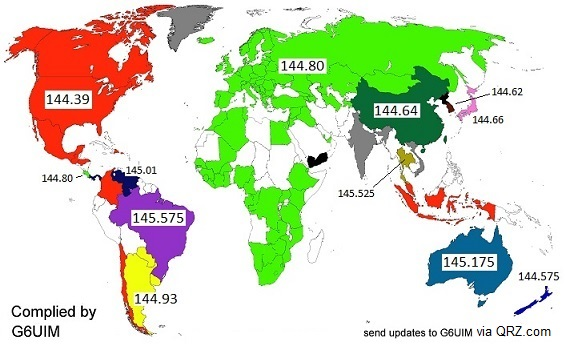
\includegraphics[width=0.65\textwidth]{Imagenes/Chapter_1/mapa_frecuencias_aprs.jpg}
	\caption{Mapa de frecuencias APRS en el mundo.}
	\label{fig:freq-map-es}
\end{figure}


\section{Usos principales de APRS}

\begin{itemize}
	\item \textbf{Reportes GPS:} APRS permite a los usuarios enviar su ubicación geográfica en forma de coordenadas, obtenida a través de sistemas GPS, lo que facilita el seguimiento de vehículos o personas en tiempo real.

	\item \textbf{Datos meteorológicos:} Las estaciones meteorológicas suelen utilizar mensajes APRS para reportar diferentes datos como temperatura, humedad o presión barométrica, incluyendo información actualizada y útil para diversas aplicaciones.

	\item \textbf{Integración con internet:} Mediante el sistema APRS-IS, los mensajes APRS son accesibles desde internet a través de distintos nodos, ampliando el alcance y la extensión de este sistema.

	\item \textbf{Uso en emergencias:} En situaciones de emergencia, APRS es una herramienta vital para la comunicación de \textit{broadcast} y el seguimiento de recursos y personal.
\end{itemize}

\section{Historia y desarrollo de APRS}

El sistema APRS nació en la década de los 80 de la mano de Bob Bruninga, un ingeniero que trabajaba en la Academia Naval de los Estados Unidos. Bruninga creó la primera implementación de APRS en un ordenador Apple II en 1982 con el objetivo de mapear informes de posición de la Marina en alta frecuencia. \cite{APRSOrigins}

El primer uso real del APRS fue en 1984, cuando Bruninga desarrolló una versión más avanzada en un VIC-20 para reportar la posición y el estado de los caballos de una carrera de resistencia.

Durante los siguientes años, Bruninga continuó perfeccionando el sistema, al que posteriormente bautizó como Sistema de Tráfico de Emergencia Sin Conexión (CETS, por sus siglas en inglés).

Tras una serie de ejercicios de la Agencia Federal de Gestión de Emergencias (FEMA) usando CETS, el sistema fue trasladado al IBM PC. Durante la década de los 90, CETS (ya conocido como el Sistema de Reporte Automático de Posición o APRS) continuó evolucionando.

A medida que la tecnología GPS se volvía más ampliamente disponible, el término ``Posición'' se reemplazó por ``Paquete'' para representar mejor las capacidades más generales del sistema y enfatizar sus usos más allá del mero reporte de posición.

\begin{figure}[h]
	\centering
	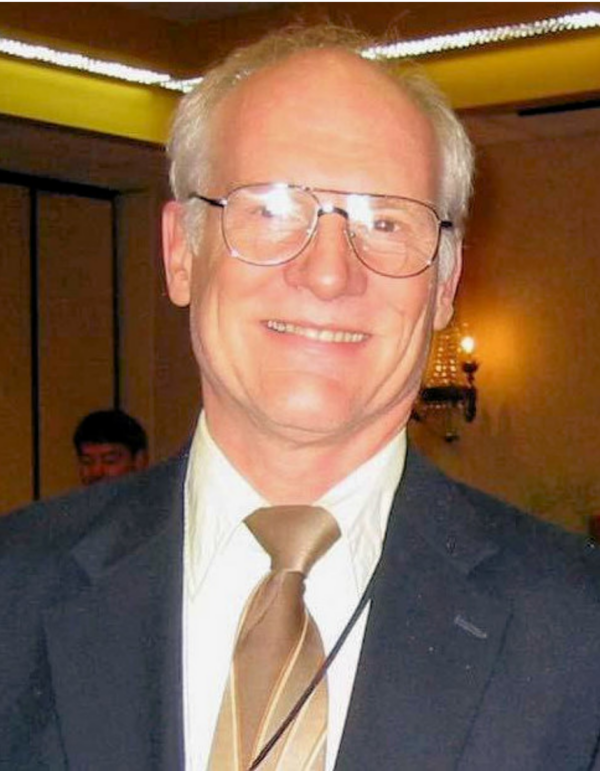
\includegraphics[width=0.2\textwidth]{Imagenes/Chapter_1/bob_bruninga.png}
	\caption{Bob Bruninga (creador del sistema APRS).}
	\label{fig:bob-bruninga-es}
\end{figure}


\section{Propuesta y objetivos}
Se propone una solución completa que incluya la adquisición, procesamiento, visualización y análisis de datos APRS. 

\subsection{Objetivos}
El objetivo del proyecto es crear una solución que mejore la experiencia del usuario y enriquezca la información APRS disponible a través de la integración de datos de diversas fuentes abiertas y disponibles.

\begin{itemize}
    \item \textbf{Mejorar la experiencia de usuario:} La solución tendrá una interfaz intuitiva, rápida y útil que facilite la navegación y la interacción con los datos.
    
    \item \textbf{Análisis avanzado:} La solución contará con herramientas avanzadas para la visualización detallada del tráfico APRS, filtrado preciso y análisis de datos, con el objetivo de extraer inteligencia de los mensajes recibidos.
    
    \item \textbf{Complementación:} La solución no tiene como objetivo sustituir a aprs.fi, aprs.to u otras plataformas similares, sino ofrecer una alternativa con funcionalidades complementarias que añadan información a los usuarios.
    
    \item \textbf{Enriquecimiento de información:} Se recopilarán datos provenientes de diversas fuentes abiertas y disponibles para ofrecer una visión más completa del tráfico APRS y sus usuarios, mejorando así la calidad de la información disponible para los usuarios.
\end{itemize}

\subsection{Beneficios}

\begin{itemize}
    \item \textbf{Mayor comprensión del tráfico APRS:} Los usuarios podrán obtener información más detallada y procesable a partir de los mensajes transmitidos, lo que les permitirá una mayor comprensión del tráfico APRS.
    
	\item \textbf{Toma de decisiones más efectiva:} El análisis de datos integrado ayudará a los usuarios a tomar decisiones más informadas haciendo uso de la información recibida, mejorando así la eficacia de sus acciones.
    
    \item \textbf{Flexibilidad:} La opción de auto-alojamiento permitirá a los usuarios tener un mayor control sobre sus datos y privacidad, proporcionando así una mayor flexibilidad en cuanto a su gestión.
\end{itemize}

\section{Requisitos}
\label{sec:Requisitos}

La solución propuesta debe cumplir con una serie de requisitos imprescindibles para asegurar su utilidad y accesibilidad:

\begin{itemize}
    \item \textbf{Bajo costo:} Debe ser una solución económica para garantizar su accesibilidad a una amplia gama de usuarios, incluidos aquellos con presupuestos limitados.
    
    \item \textbf{Flexibilidad de alojamiento:} Se debe ofrecer la capacidad de auto-alojamiento, los usuarios deben poder optar por alojarla en sus propios servidores o usar la solución en la nube según sus preferencias y requisitos específicos.
    
    \item \textbf{Extensible:} La solución debe ser extensible, lo que significa que debe permitir la integración de nuevas funcionalidades y la expansión de su capacidad según las necesidades cambiantes de los usuarios.
    
    \item \textbf{Mejor filtrado:} Se debe ofrecer un filtrado más preciso y flexible en comparación con las plataformas existentes, lo que permitirá a los usuarios obtener información relevante y útil de los datos APRS para complementar la ya provista por las alternativas.
    
	\item \textbf{Análisis de datos integrado:} La solución debe incluir un análisis de datos integrado para ayudar a los usuarios a comprender mejor la información recibida a través del APRS y obtener perspectivas y conclusiones valiosas a partir de los mensajes transmitidos.
	
\end{itemize}

\section{Plan de trabajo}

Para la realización de este proyecto se ha propuesto el siguiente plan de trabajo, que se divide en las siguientes fases:

\begin{itemize}
	\item \textbf{Fase 1:} Investigación y Análisis de Requisitos.
	\item \textbf{Fase 2:} Diseño y Planificación.
	\item \textbf{Fase 3:} Implementación y Desarrollo.
	\item \textbf{Fase 4:} Realización de la memoria.
\end{itemize}

\noindent En la figura \Cref{fig:gantt-diagram-es} se muestra el diagrama de Gantt con las fechas de inicio y fin de cada una de las actividades que se han llevado a cabo a lo largo del proyecto.

\begin{figure}[h]
	\centering
	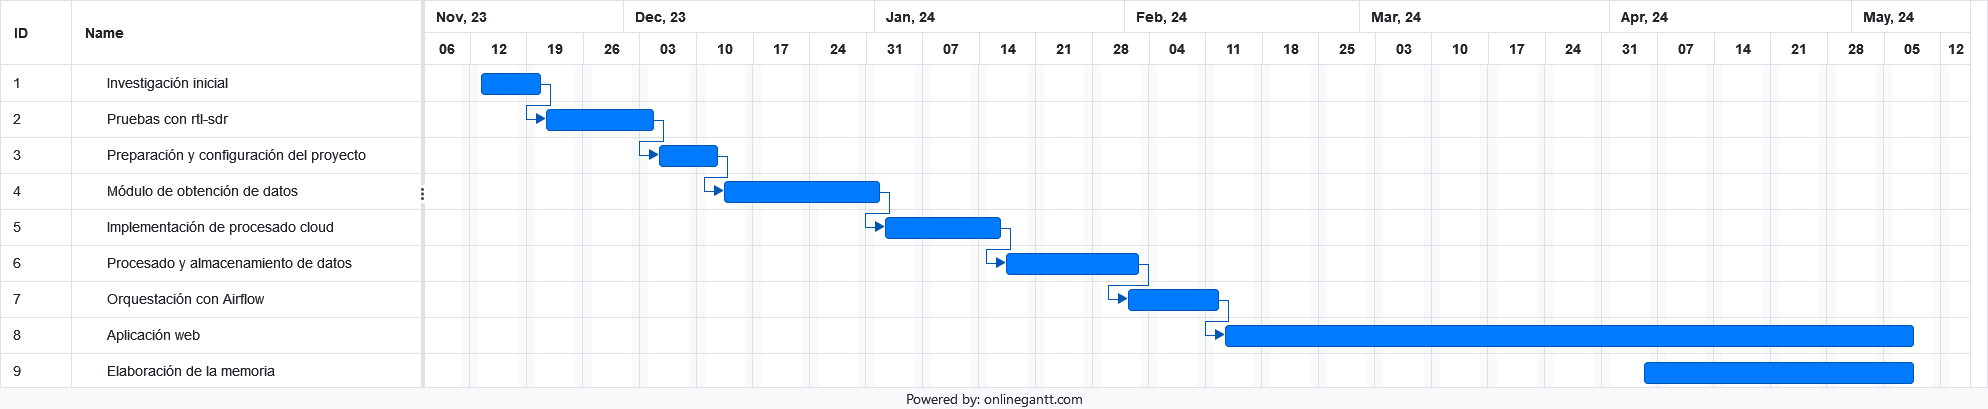
\includegraphics[width=1\textwidth]{Imagenes/Chapter_1/gant.png}
	\caption{Plan de trabajo propuesto.}
	\label{fig:gantt-diagram-es}
\end{figure}

\noindent También se han realizado reuniones periódicas con los directores de TFG para revisar el progreso y discutir los problemas encontrados durante el desarrollo.
\titleformat{\chapter}[display]
{\normalfont\huge\bfseries}{Capítulo \thechapter}{0.5em}{\huge}
\titlespacing*{\chapter}{0pt}{-1.25cm}{25pt}
\chapter{Contexto del problema y estado del arte}

\section{Contexto del problema}

El \textit{Automatic Packet Reporting System} (APRS) como sistema de comunicación digital se basa en la gran comunidad de radioaficionados e incluso tiene aplicaciones industriales como la transmisión de información en tiempo real de vehículos logísticos o estaciones de meteorología. A pesar de su versatilidad y flexibilidad, el APRS presenta algunas barreras de entrada para usuarios que no pertenecen a la comunidad radioaficionada o tienen sólidos conocimientos de este ámbito. En este capítulo, se analizarán estas barreras y se discutirán los requisitos necesarios.

\subsection{Barreras de entrada}

El APRS requiere conocimientos básicos sobre radiocomunicación y la obtención de una licencia de radioaficionado en caso de querer emitir. La obtención de la licencia a pesar de no implicar un desembolso económico importante, si que requiere un estudio y comprensión de los sistemas y legislación pertinente.

Adicionalmente, el APRS utiliza una estructura de mensaje específico y un conjunto de protocolos que pueden ser difíciles de entender para usuarios no familiarizados con este tipo de tecnología. La falta de documentación y antigüedad de esta hacen que desarrollar soluciones para este sistema sea complicado.

\subsection{Hardware}

Para utilizar APRS, se necesita hardware especializado que incluya un transceptor de radio, un \textit{Terminal Node Controller} (TNC) y un dispositivo GPS (opcionalmente), existen otras opciones más baratas como los dispositivos \textit{software defined radio} o RTL-SDR \Cref{fig:rtl-sdr} que se conectan directamente a un ordenador. Los TNC son dispositivos que convierten las señales digitales emitidas por un ordenador en señales de radio y viceversa. El dispositivo GPS proporciona información de ubicación que se puede transmitir junto con otros datos en el cuerpo del mensaje.

El precio del hardware APRS puede variar dependiendo de la calidad y las características del equipo. Sin embargo, a pesar de no contar con precios prohibitibamente altos, la inversión que supone conlleva el hecho de que solamente los usuarios con un interés previo en la radioafición o la tecnología en general estén dispuestos a adquirirlo.

\begin{figure}
    \centering
    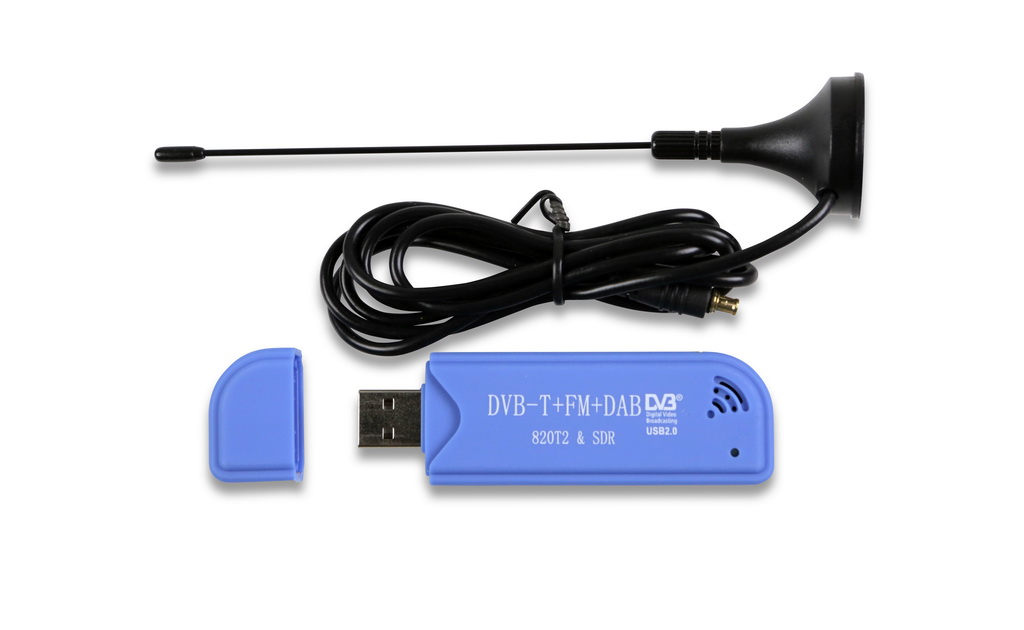
\includegraphics[width=0.5\textwidth]{Imagenes/Chapter_2/rtl_sdr.jpg}
    \caption{Ejemplo de un RTL-SDR de tipo usb.}
    \label{fig:rtl-sdr}
\end{figure}


\subsection{OSINT y APRS}

El APRS sirve como una herramienta de comunicación para los radioaficionados y de reporte de telemetría para las industrias. Pero se puede convertir en una valiosa fuente de información para la obtención de inteligencia (OSINT). Esto se debe a su capacidad para proporcionar una gran cantidad de datos en tiempo real sobre ubicación y estado de los activos así como una amplia gama de información adicional.

En el ámbito del OSINT, el APRS ofrece una serie de aplicaciones prácticas. Por ejemplo, los datos APRS son actualmente utilizados para el rastreo de vehículos en tiempo real, lo que resulta muy útil para empresas de logística y transporte. Además, la red APRS se utiliza para monitorear la actividad de estaciones meteorológicas, proporcionando datos en tiempo real sobre condiciones climáticas locales. También se utiliza en situaciones de emergencia, como pueden ser desastres naturales o incidentes críticos, el APRS desempeña un papel crucial al permitir la transmisión rápida de información sobre ubicaciones de refugios, recursos disponibles y necesidades de ayuda, ya que no depende necesariamente de infraestructura de una entidad como si lo hace la red telefónica.

Aunque el APRS tiene un gran potencial para aplicaciones en el ámbito del OSINT, su uso en esta área es prácticamente inexistente. Este hecho puede explicarse en parte por las barreras de entrada mencionadas anteriormente, que incluyen la necesidad de poseer conocimientos especializados en radiocomunicación, obtener licencias de radioaficionado y adquirir hardware especializado.

\section{Estado del Arte}

Existen varios sitios web que ofrecen servicios relacionados con APRS, entre los cuales destacan \textbf{aprs.fi} y \textbf{aprs.to} probablemente las dos webs más grandes.

\subsection{aprs.fi}

aprs.fi es una de las webs más utilizadas para visualizar datos APRS en tiempo real y acceder a un histórico extenso de información. Sin embargo, su interfaz puede considerarse un tanto desactualizada (ver \Cref{fig:aprs-fi}), lo que puede dificultar la navegación y la búsqueda de información específica. Aunque ofrece una gran cantidad de datos y un histórico significativo, la plataforma carece de capacidades avanzadas de filtrado de estaciones y mensajes. Además, para acceder a funciones más complejas y realizar extracciones de datos, es necesario crear una cuenta.

\begin{figure}[h]
    \centering
    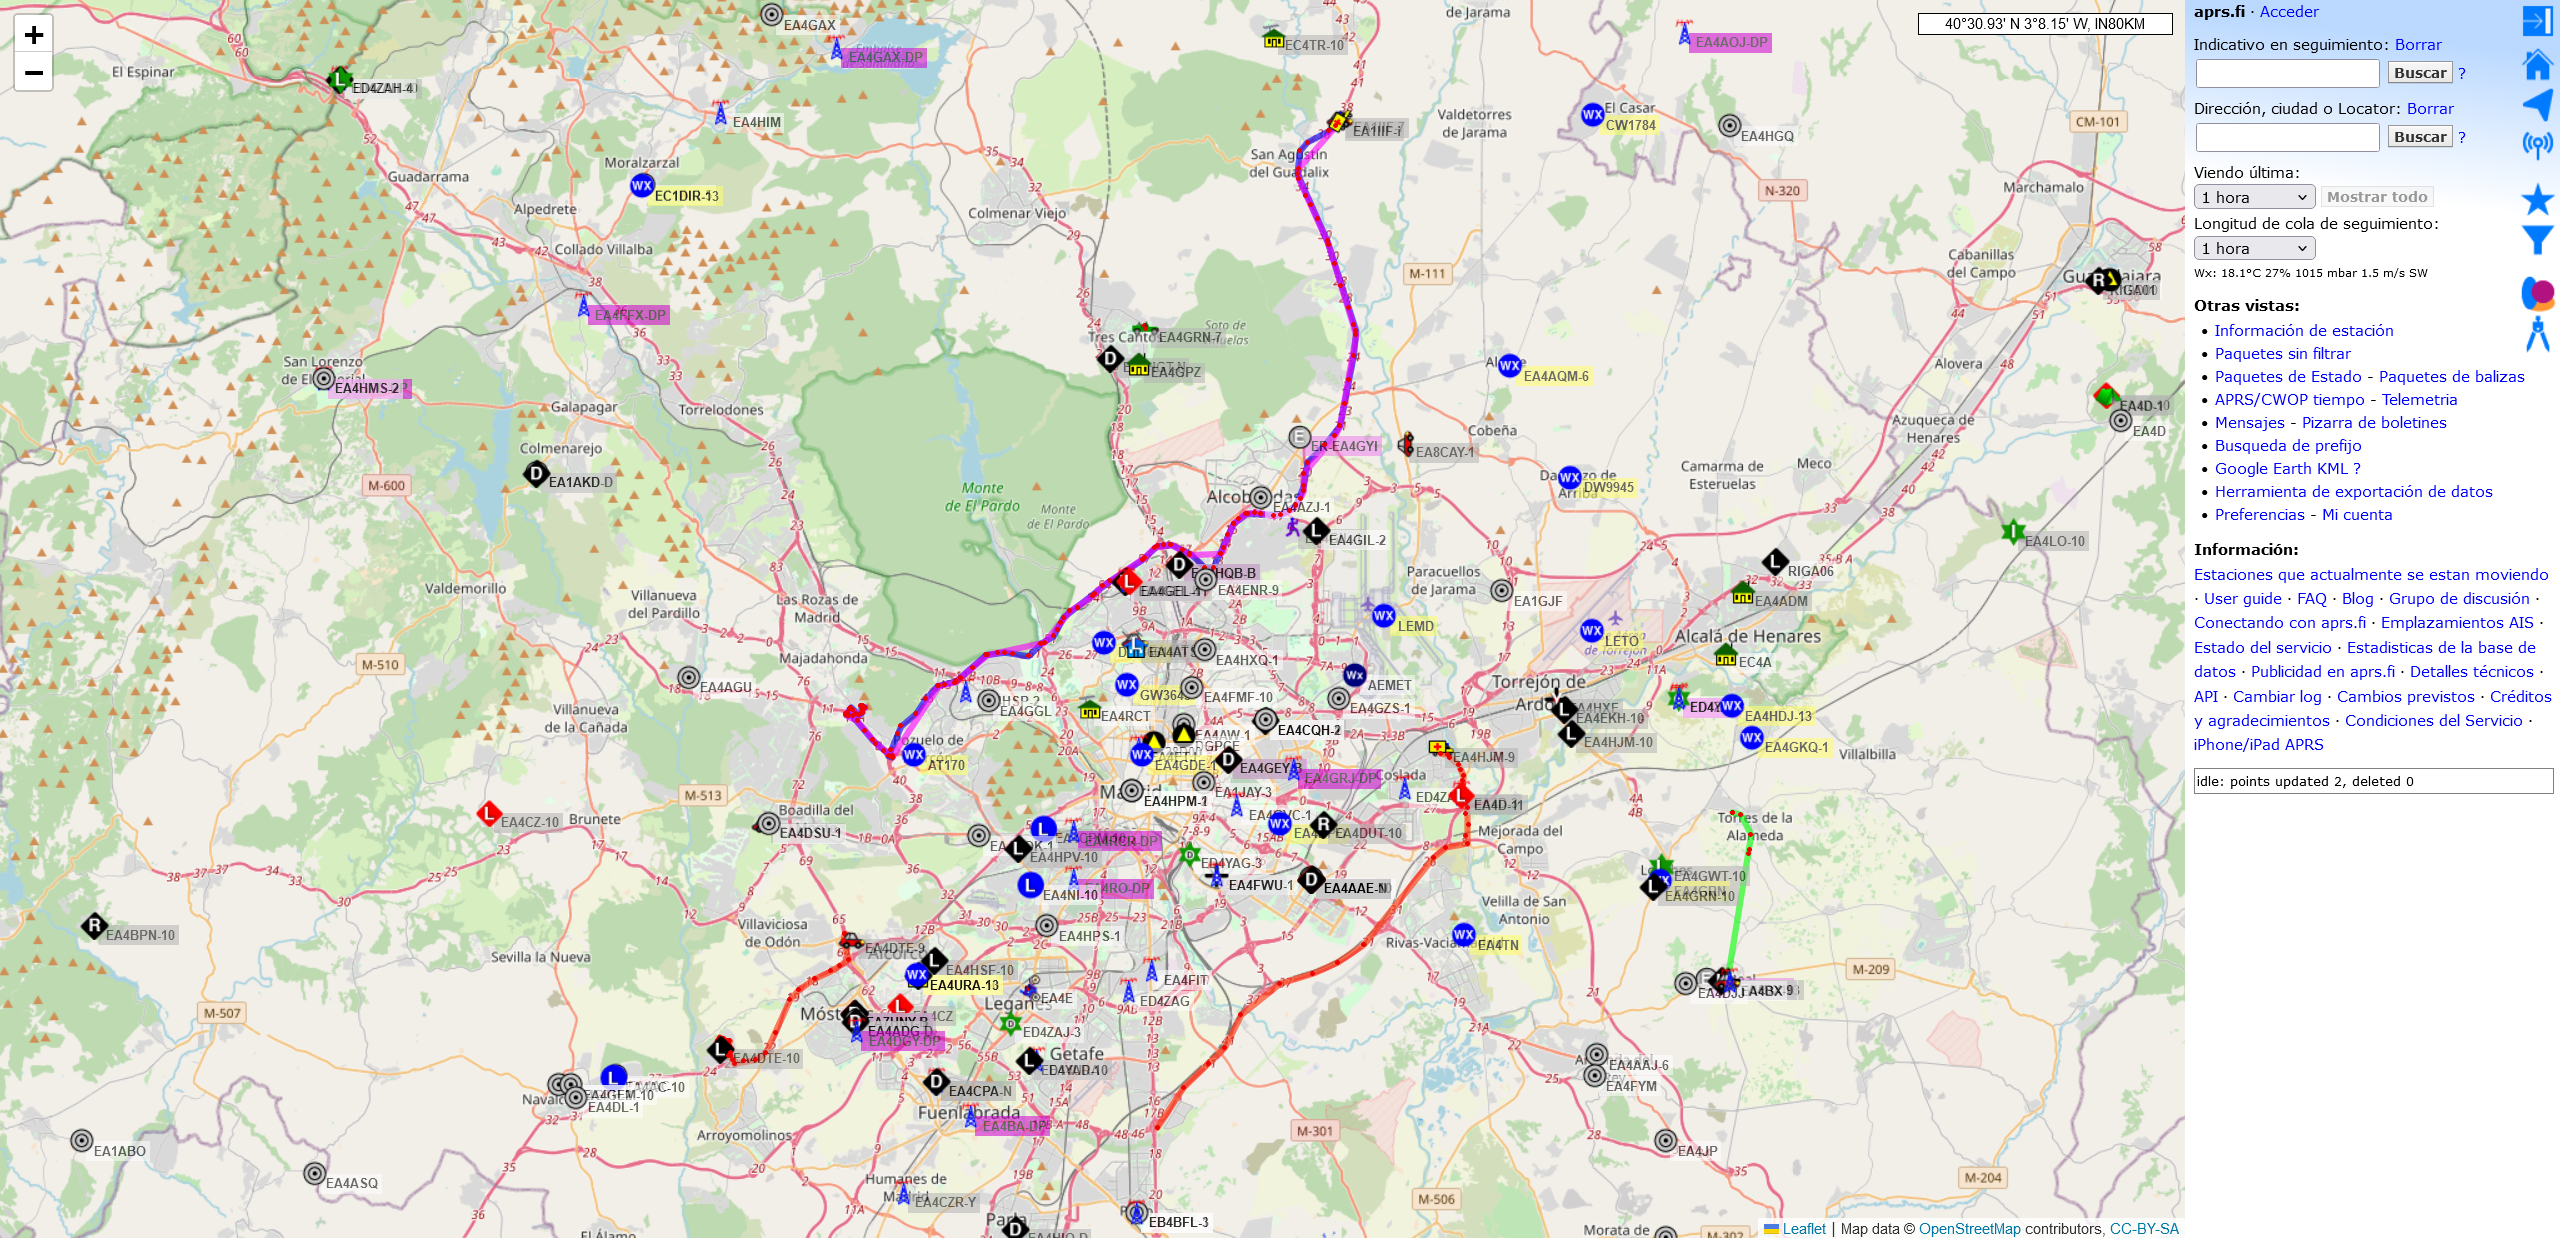
\includegraphics[width=0.7\textwidth]{Imagenes/Chapter_2/aprs-fi.png}
    \caption{Interfaz de aprs.fi}
    \label{fig:aprs-fi}
\end{figure}

\subsection{aprs.to}

Por otro lado, aprs.to ofrece una interfaz más moderna y cuidada (ver \Cref{fig:aprs-to}), lo que facilita la navegación y la búsqueda de información. Además, permite realizar búsquedas básicas y aplicar filtros para refinar los resultados. Sin embargo, al igual que aprs.fi, también requiere que los usuarios se creen una cuenta para acceder a ciertas funcionalidades avanzadas.

\begin{figure}[h]
    \centering
    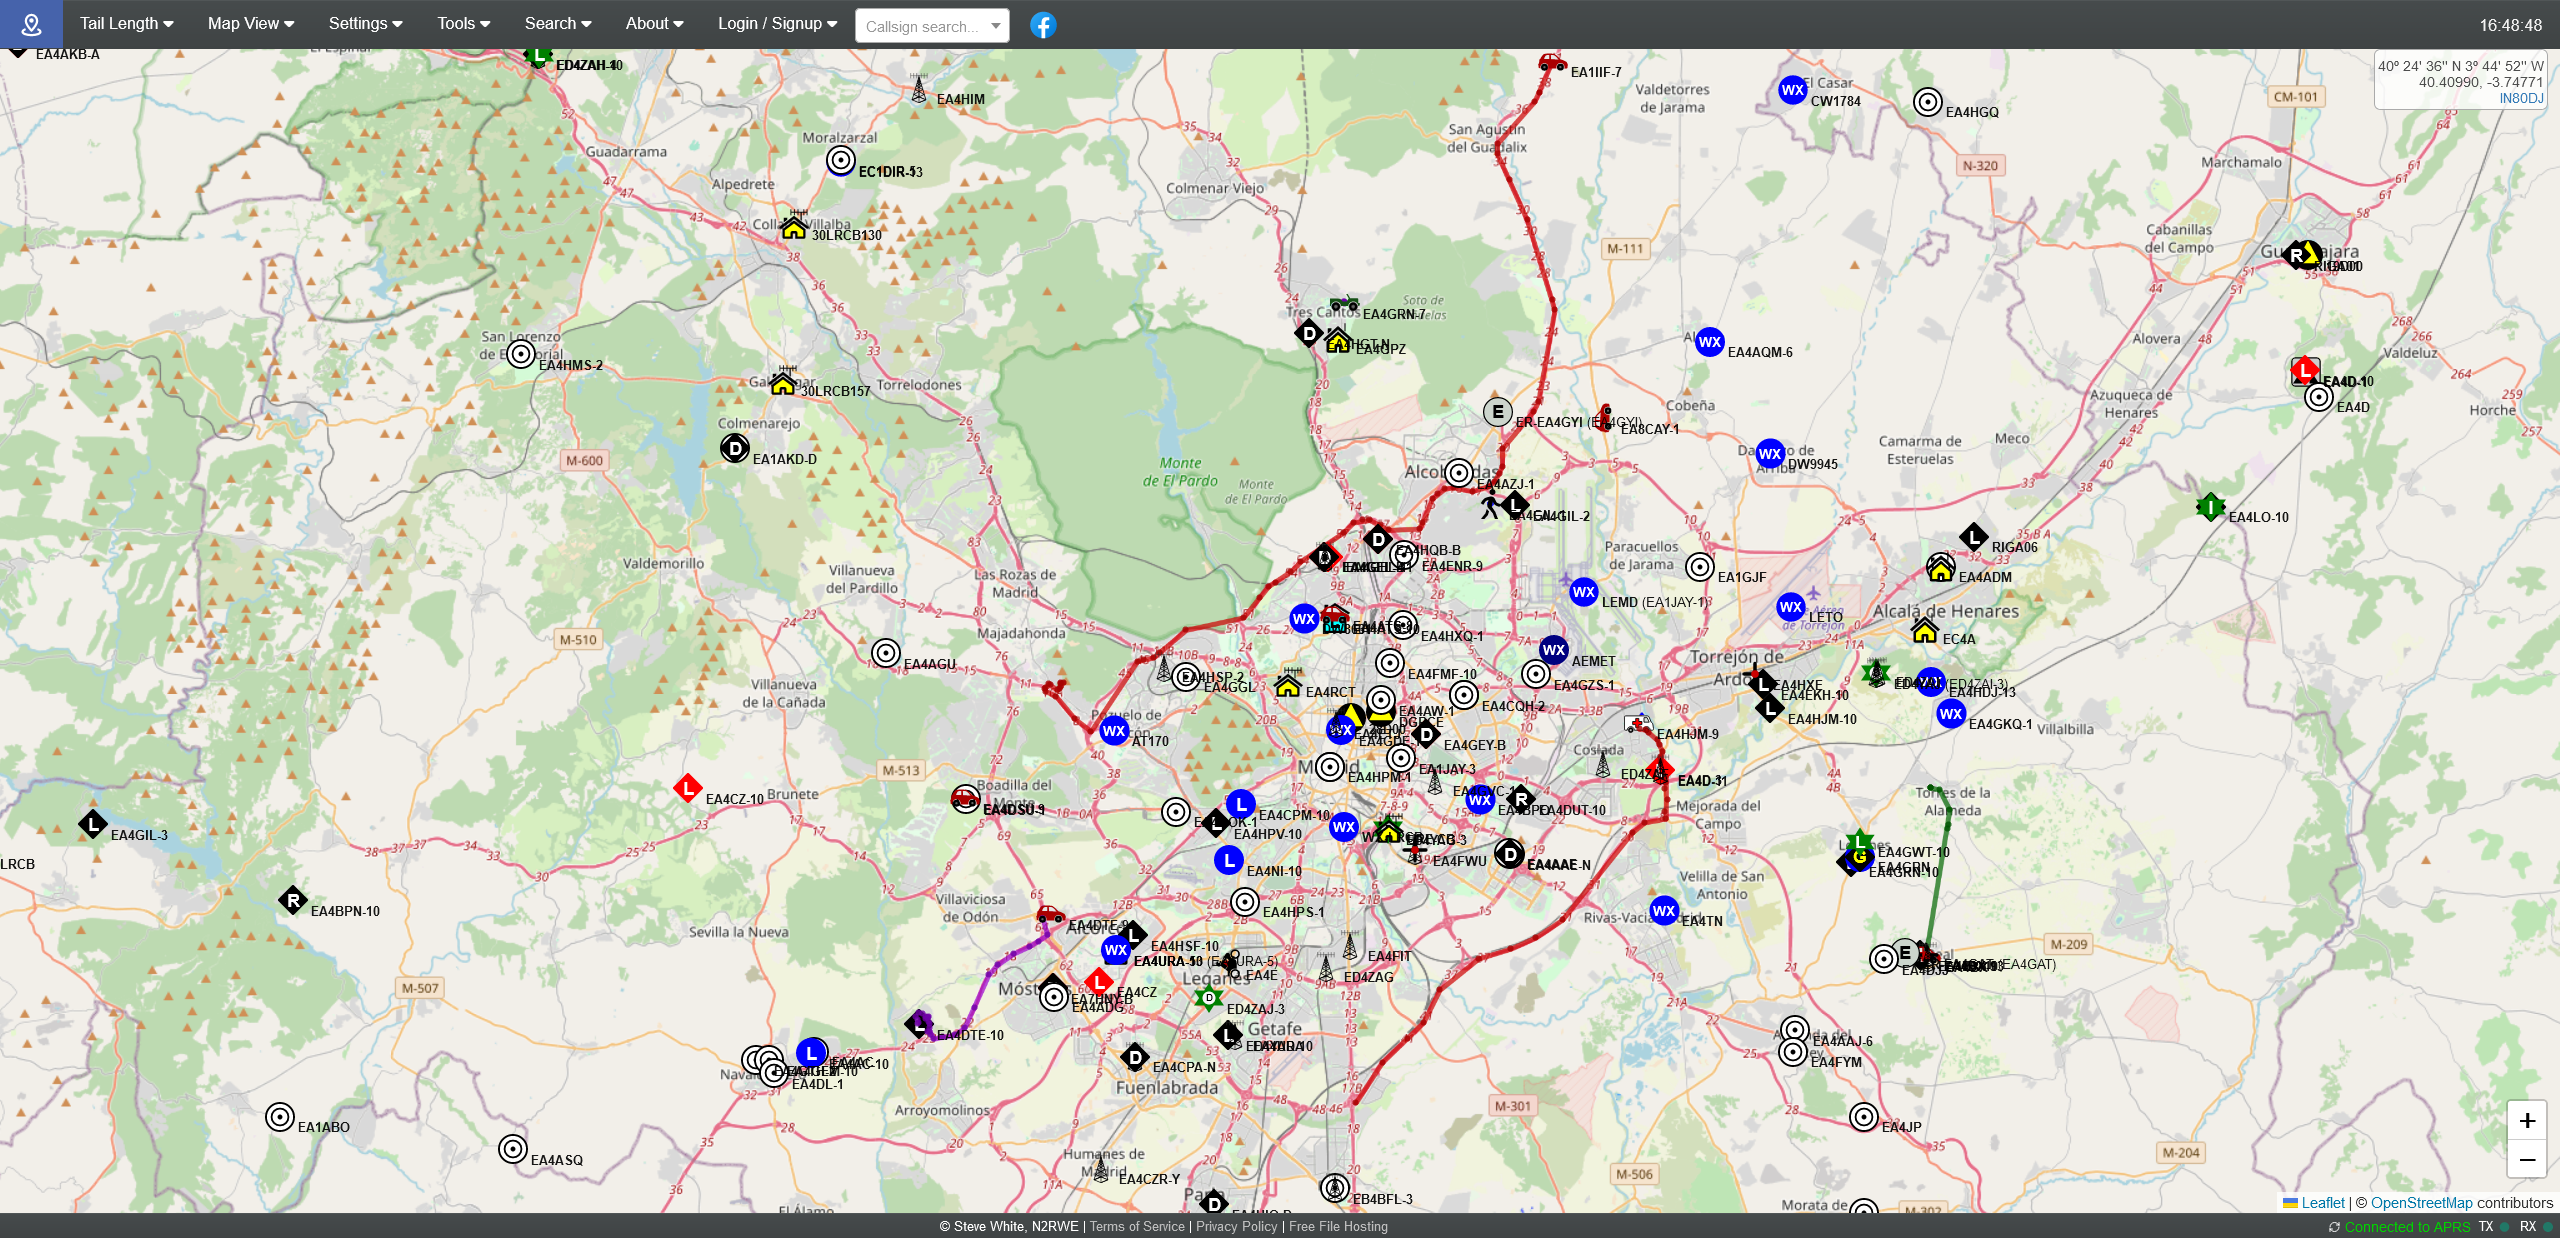
\includegraphics[width=0.7\textwidth]{Imagenes/Chapter_2/aprs-to.png}
    \caption{Interfaz de aprs.to}
    \label{fig:aprs-to}
\end{figure}

\subsection{Comparación}

En resumen, aprs.fi, la web de visualización de APRS por excelencia, ofrece una gran base de datos y una gran cantidad de información histórica de datos APRS, pero su interfaz puede resultar algo desactualizada y carece de capacidades avanzadas de filtrado. Por otro lado, aprs.to presenta una interfaz más moderna y permite realizar búsquedas básicas y aplicar filtros, aunque también requiere crear una cuenta para acceder a ciertas funciones. Ambas plataformas tienen puntos fuertes y débiles y por esa razón lo mejor es usarlas en conjunto.

\chapter{Descripción del Trabajo}
\label{cap:descripcionTrabajo}

En este capítulo se describen los módulos que conforman la aplicación así como la arquitectura y las tecnologías utilizadas para su implementación.
\section{APRSINT}
La solución propuesta se ha llamado \textbf{APRSINT}, que es una combinación de los acrónimos APRS y OSINT. APRSINT está dividida en tres módulos principales:
\begin{itemize}
	\item \textbf{Adquisición de datos:} Este módulo se encargará de recopilar y almacenar los mensajes APRS de diversas fuentes, así como de integrar datos de otras fuentes abiertas y disponibles.
	\item \textbf{Procesamiento y análisis:} Este módulo se encargará de procesar y analizar los datos recopilados, ofreciendo herramientas avanzadas de visualización, filtrado y análisis de datos.
	\item \textbf{Visualización y presentación:} Este módulo se encargará de presentar los datos procesados y analizados de forma clara y comprensible, facilitando la interpretación y la toma de decisiones.
\end{itemize}

\begin{figure}[h]
	\centering
	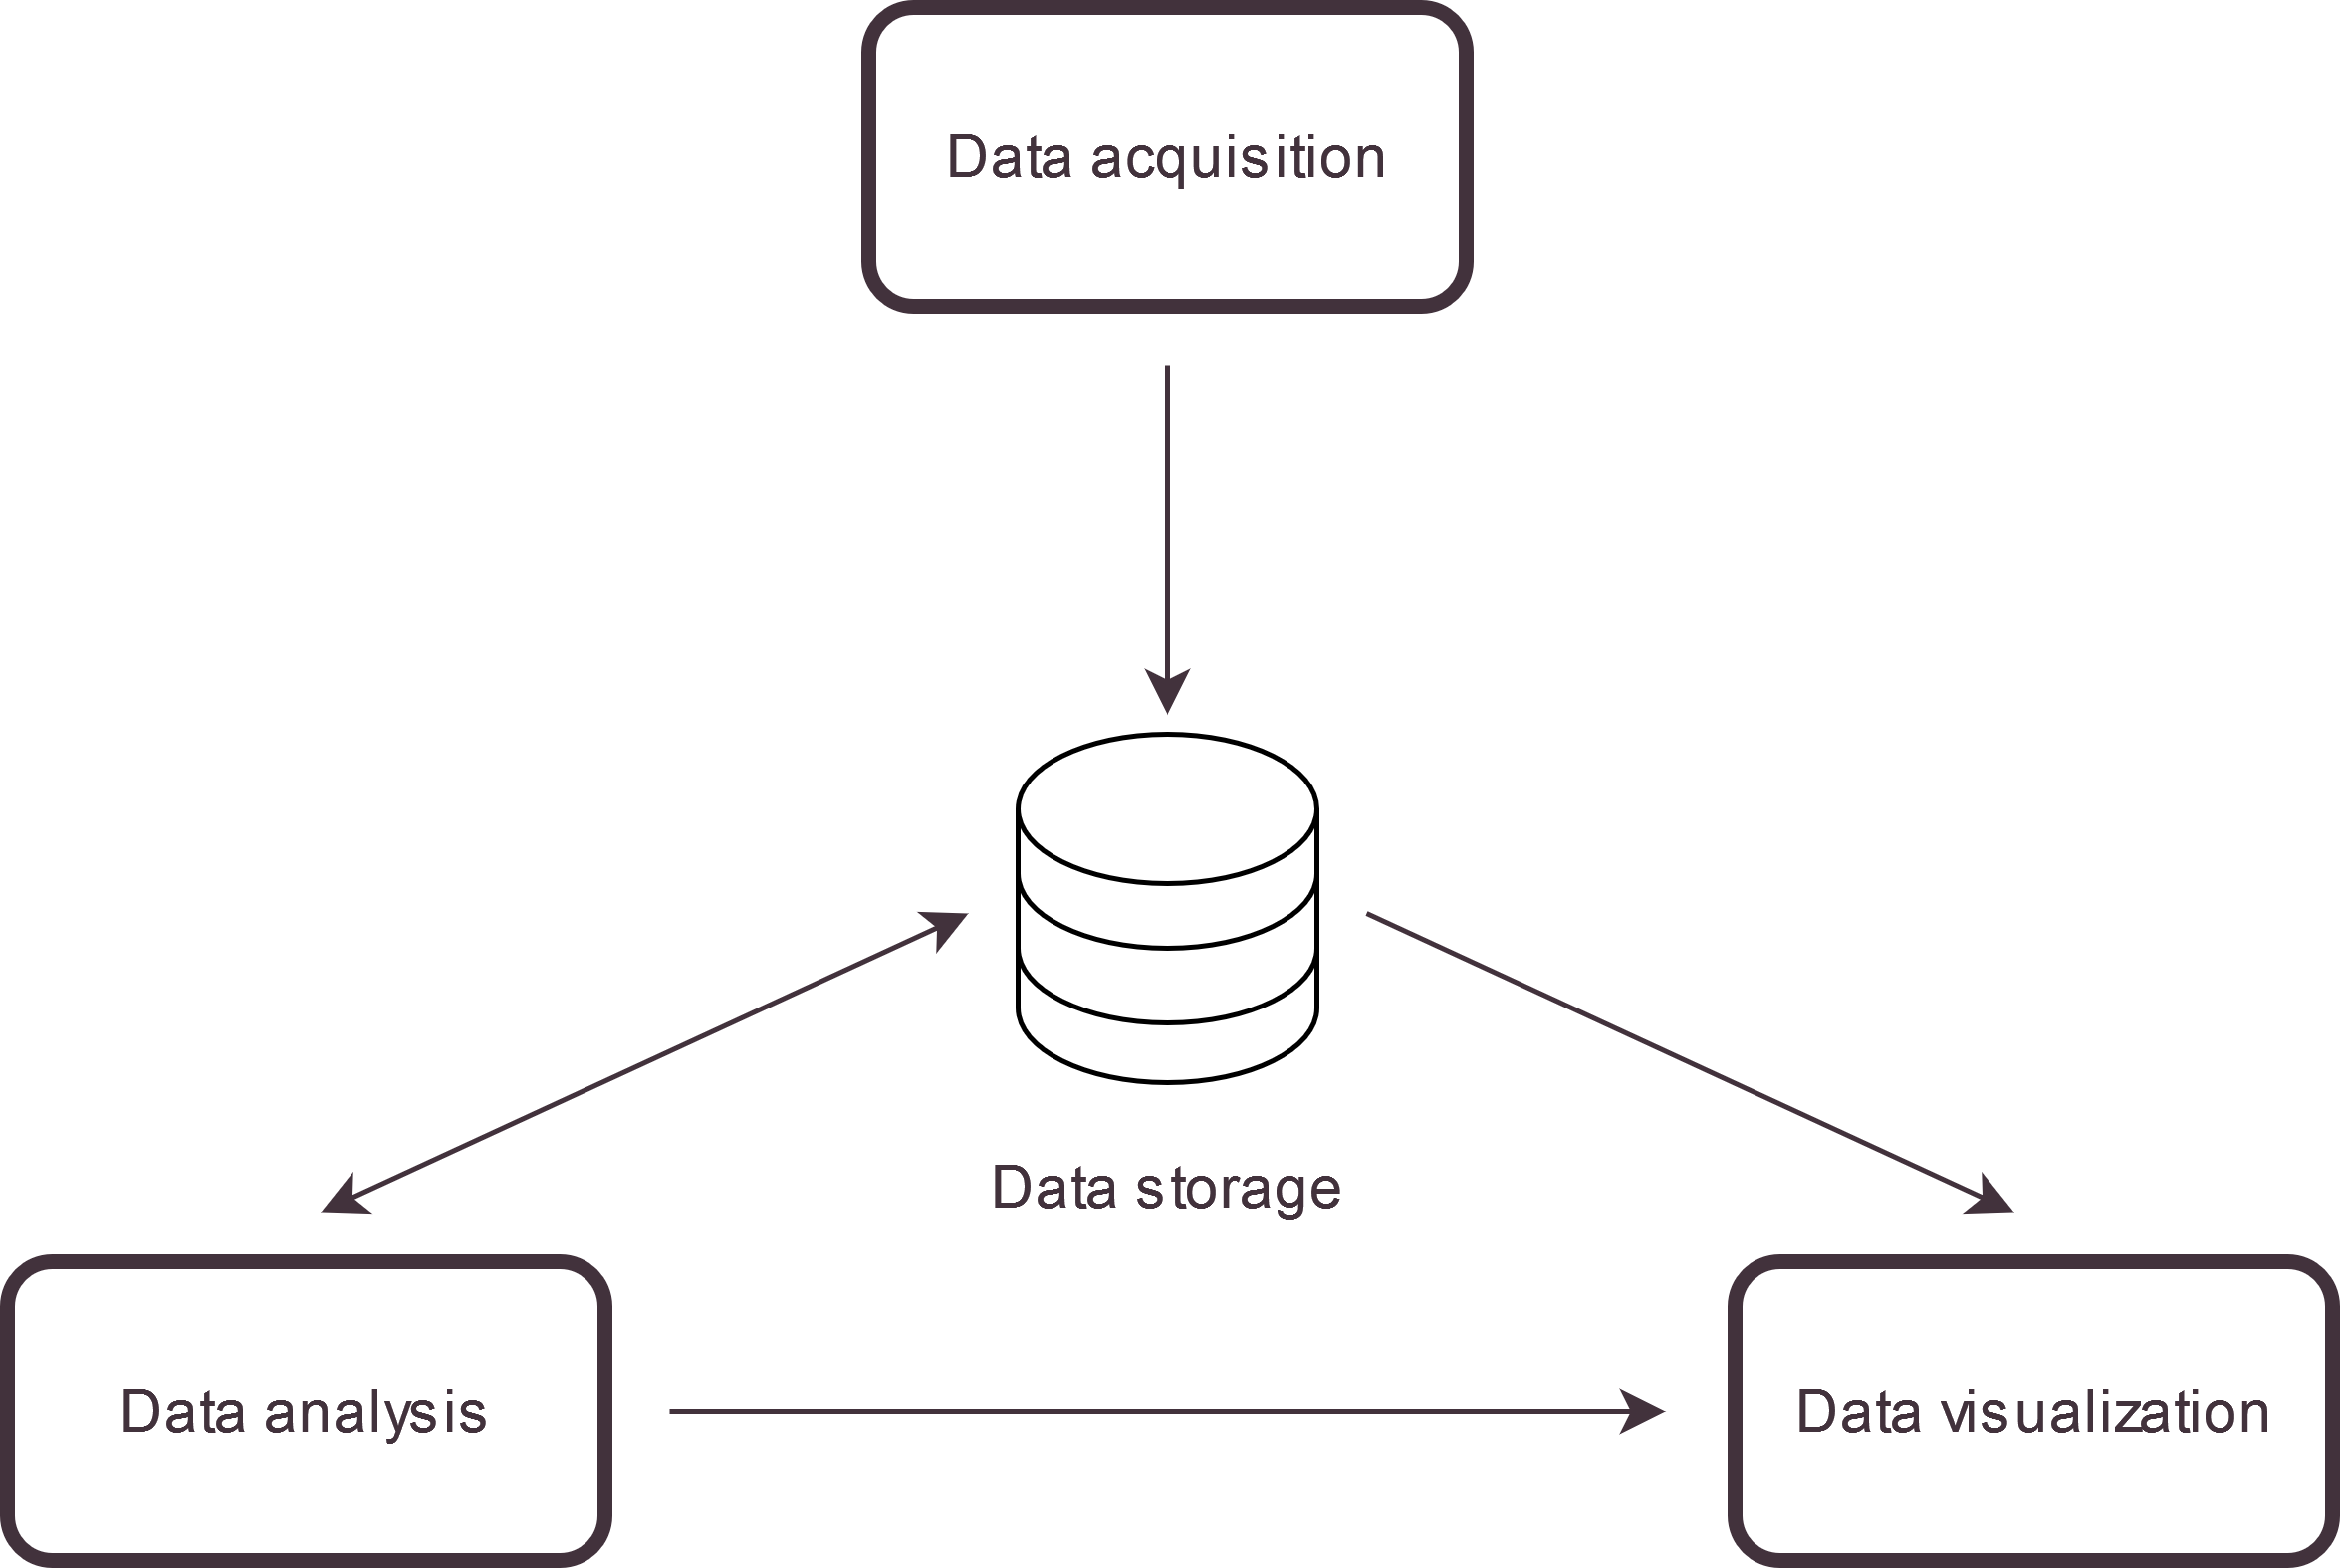
\includegraphics[width=0.52\textwidth]{Imagenes/Chapter_3/structure.png}
	\caption[Módulos de de la aplicación]{Módulos de de la aplicación (elaboración propia).}
	\label{fig:aprsint-logo}
\end{figure}

\FloatBarrier

\section{Arquitectura de la aplicación}

Se pueden categorizar los tres módulos (\textbf{Adquisición de datos}, \textbf{Procesamiento y análisis}, \textbf{Visualización y presentación}) de la aplicación mencionados previamente en dos categorías principales:

\begin{itemize}
	\item \textbf{Adquisición de paquetes APRS:} En este módulo se encuentran los componentes encargados de la adquisición de paquetes APRS. Estos componentes se encargan de recibir los paquetes APRS, procesarlos y almacenarlos en la base de datos de la aplicación.

	\item \textbf{Aplicación web APRSINT:} En este módulo se encuentran los componentes encargados del análisis, la interpretación y la visualización, de los datos almacenados en la base de datos de la aplicación. Estos componentes se encargan de presentar la información de manera rápida y cómoda para el usuario.
\end{itemize}

\section{Tecnologías utilizadas y marco teórico}

Como se ha mencionado anteriormente, uno de los objetivos de APRSINT es el de ser una solución accesible y fácil de usar. Para lograr este objetivo, se han seleccionado tecnologías ampliamente utilizadas y bien documentadas. A continuación se describen las tecnologías utilizadas en cada uno de los módulos de la aplicación.
\subsection{Raspberry Pi}

La Raspberry Pi es un \textit{Single board computer (SBC)} u ordenador de placa única desarrollada por la Fundación Raspberry Pi. Las Raspberry Pi son muy populares en el mundo de la informática y la electrónica por su bajo precio, reducido tamaño y su versatilidad.

\begin{itemize}
	\item \textbf{Bajo precio:} La Raspberry es una opción económica para implementar desde prototipos hasta aplicaciones simples, lo que la hace muy accesible para una amplia gama de usuarios.
	\item \textbf{Bajo consumo energético:} Su diseño de bajo consumo energético la hace ideal para aplicaciones que requieren funcionamiento continuo.
	\item \textbf{Versatilidad:} La Raspberry Pi 4 es altamente versátil y puede adaptarse a una variedad de casos de uso, desde servidores ligeros hasta placas de desarrollo para robótica y automatización.
\end{itemize}

\noindent Se ha seleccionado la Raspberry Pi 4B\footnote{Cuando se comenzó el proyecto todavía no se había lanzado la versión 5.} de 8GB de memoria RAM como plataforma de hardware para la implementación de la solución, debido a sus características y capacidades.

\subsection{Disco duro SSD}
Los discos duros de estado sólido (SSD) son una alternativa a los discos duros tradicionales (HDD) que ofrecen una mayor velocidad de lectura y escritura, menor consumo energético y mayor durabilidad. Se ha seleccionado un disco duro SSD de 250GB que se haya conectado a la Raspberry-pi para almacenar el gran volumen de datos que consume y genera la aplicación a su velocidad y fiabilidad.

\subsection{Python}
Python es un lenguaje de programación interpretado, de alto nivel y de propósito general. Es ampliamente utilizado en el desarrollo de aplicaciones web, científicas y de análisis de datos debido a su simplicidad, flexibilidad y facilidad de uso. Se ha seleccionado Python como lenguaje de programación principal para la implementación de la solución debido a la gran versatilidad que ofrece y sobre todo por la existencia de extensas librerías de visualización y manejo de grandes volúmenes de datos.

\subsection{Dash}
Dash es un \textit{framework} creado por Plotly que permite crear ``dashboards'', aplicaciones web interactivas y visualizaciones de datos atractivas utilizando Python como lenguaje de programación. Se ha seleccionado Dash como \textit{framework} para la implementación de la interfaz web de la aplicación debido a su facilidad de uso y a la gran cantidad de funcionalidades que ofrece. Dash está escrito encima de Plotly.js, React y Flask lo que permite una gran capacidad de personalización.

\begin{itemize}
	\item \textbf{Interactividad:} Dash permite crear aplicaciones web altamente interactivas, lo que facilita la exploración de datos y la toma de decisiones.
	\item \textbf{Flexibilidad:} Su arquitectura modular y su amplia gama de componentes permiten la creación de aplicaciones web personalizadas y adaptadas a las necesidades específicas del usuario.
	\item \textbf{Integración con Plotly:} Al estar desarrollado por Plotly, Dash ofrece una integración perfecta con las capacidades de visualización de datos de Plotly, lo que permite crear gráficos y visualizaciones muy atractivas.
\end{itemize}

\noindent Para crear la aplicación web se consideraron algunas alternativas como Django, Streamlit y PowerBI, sin embargo, Dash fue la opción escogida debido a su extensa capacidad de personalización de la que carecían las demás opciones.

\subsection{Cosmograph JS}

Cosmograph es una librería de JavaScript enfocada en la visualización de grandes grafos y redes complejas en aplicaciones web. Permite representar de manera interactiva relaciones entre entidades, facilitando la comprensión y el análisis de datos estructurados.

\begin{itemize}
	\item \textbf{Visualización de grafos:} Cosmograph ofrece herramientas avanzadas para la representación visual de grafos como lineas temporales, histogramas y búsquedas de nodos, una mayor comprensión y capacidad de análisis de la información.

	\item \textbf{Rendimiento:} Cosmograph a diferencia de otras librerías más populares como Sigma JS transfiere todos los cálculos de posiciones de los nodos y aristas así como la representación gráfica de este a la GPU. Esto permite la visualización de grafos con miles de nodos y aristas sin afectar el rendimiento de la aplicación.

	\item \textbf{Personalización:} Ofrece opciones de personalización para adaptar la apariencia y el comportamiento de los nodos y aristas según las necesidades específicas del usuario.

\end{itemize}

\noindent Después de una gran cantidad de pruebas y tras considerar muchas alternativas como Sigma-JS, CytoScape y networkx, se acabó eligiendo Cosmograph sobre todo por su rendimiento.

\subsection{PostgreSQL}

PostgreSQL es un sistema de gestión de bases de datos relacional de código abierto y potente, conocido por su fiabilidad, robustez y capacidad para manejar grandes volúmenes de datos. Ofrece una amplia gama de características avanzadas que lo hacen adecuado para aplicaciones web y científicas que requieren almacenamiento y manipulación de datos complejos.

\begin{itemize}
	\item \textbf{Fiabilidad y robustez:} PostgreSQL es conocido por su alta fiabilidad y capacidad para manejar grandes cargas de trabajo sin disminuir el rendimiento.
	\item \textbf{Escalabilidad:} Es altamente escalable y puede manejar grandes volúmenes de datos y transacciones concurrentes sin problemas.
	\item \textbf{Funcionalidades avanzadas:} Ofrece una amplia gama de funcionalidades avanzadas, como soporte para transacciones ACID, vistas materializadas, procedimientos almacenados y Full Text Search (búsqueda indexada).
	\item \textbf{Almacenamiento de datos semiestructurados:} PostgreSQL es capaz de almacenar y manipular datos no estructurados como JSON de manera eficiente, lo que lo hace adecuado para aplicaciones que requieren almacenamiento de datos semiestructurados.
	\item \textbf{Rendimiento:} PostgreSQL ofrece un muy buen rendimiento, especialmente en entornos de alta concurrencia y cargas de trabajo intensivas.
\end{itemize}

\noindent La elección de PostgreSQL como sistema de gestión de bases de datos se debió a su robustez, facilidad de uso y a la gran cantidad de funcionalidades que ofrece.

\subsection{SQLAlchemy}
SQLAlchemy es una biblioteca de Python que facilita la interacción con bases de datos relacionales utilizando un enfoque orientado a objetos. Permite trabajar con diferentes motores de bases de datos, como PostgreSQL, MySQL, SQLite, entre otros, de una manera consistente y eficiente.

\begin{itemize}
	\item \textbf{Abstracción de la base de datos:} SQLAlchemy proporciona una capa de abstracción sobre la base de datos, esto permite interactuar con la base de datos utilizando objetos de Python en lugar de consultas SQL directas.
	\item \textbf{Compatibilidad con múltiples motores:} Es compatible con una muchos motores de bases de datos, lo que brinda flexibilidad para trabajar con diferentes sistemas según las necesidades del proyecto. En este caso se ha utilizado el motor \textit{Psycopg3} para la conexión con PostgreSQL.
	\item \textbf{ORM (mapeo objeto-relacional):} Ofrece un ORM potente y flexible que mapea objetos Python a tablas de bases de datos, facilitando el manejo de relaciones entre objetos y la persistencia de datos.
	\item \textbf{Seguridad:} SQLAlchemy proporciona herramientas para prevenir ataques de inyección SQL y otros problemas de seguridad comunes a las bases de datos.
\end{itemize}

\noindent La elección de SQLAlchemy se ha basado en su capacidad para mejorar el proceso de interacción con la base de datos. Proporciona una estrecha integración entre la base de datos y la aplicación, permitiendo una flexibilidad muy grande a la hora de hacer consultas o inserciones y sobre todo creando una capa de seguridad para evitar ataques.

\subsection{Aprslib}
Aprslib es una biblioteca de Python que facilita la interacción con el sistema y la red APRS. Permite recibir, enviar y decodificar paquetes APRS a través de la red APRS-IS.
\begin{itemize}
	\item \textbf{Recepción de paquetes:} Aprslib permite recibir paquetes APRS de la red APRS-IS de manera sencilla mediante la conexión con los servidores centrales de APRS-IS.
	\item \textbf{Decodificación de paquetes:} Facilita la decodificación de paquetes APRS, permitiendo extraer información útil como la posición, velocidad y rumbo de los objetos rastreados.
	\item \textbf{Envío de paquetes:} Aprslib permite enviar paquetes APRS a través de la red APRS-IS, lo que facilita la integración con el sistema APRS.
\end{itemize}
\noindent Se ha elegido la librería Aprslib por su facilidad de uso, su documentación y su capacidad para decodificar los paquetes APRS.

\subsection{AWS}
\textit{Amazon Web Services} (AWS) es una plataforma de servicios en la nube ofrecida por Amazon. Proporciona servicios de infraestructura informática, almacenamiento, bases de datos, análisis e inteligencia artificial, entre otros.

\begin{itemize}
	\item \textbf{Fiabilidad:} La infraestructura global de AWS está diseñada para ser altamente disponible y resistente a fallos, lo que garantiza la continuidad del servicio y la seguridad de los datos.
	\item \textbf{Variedad de servicios:} AWS ofrece una amplia gama de servicios, desde almacenamiento y bases de datos hasta aprendizaje automático y análisis de datos, lo que permite a las empresas construir y desplegar una amplia variedad de aplicaciones y soluciones.
	\item \textbf{Flexibilidad:} AWS proporciona opciones flexibles de implementación, incluyendo la capacidad de utilizar infraestructura física, virtual o basada en contenedores, según las necesidades del proyecto.
	\item \textbf{Seguridad:} AWS cuenta con medidas de seguridad muy robustas para proteger los datos y las aplicaciones, incluyendo controles de acceso, cifrado de datos y protección contra amenazas.
\end{itemize}

\noindent La elección de AWS así como los detalles de la implementación en la nube se describirán en la siguiente sección.

\subsection{Supervisord}
Supervisord es un sistema de control de procesos para sistemas operativos tipo Unix, diseñado para iniciar, detener y gestionar procesos de manera sencilla y robusta. Permite supervisar y mantener en funcionamiento aplicaciones y servicios, reiniciándolos automáticamente en caso de fallos o reinicios del sistema.

\begin{itemize}
	\item \textbf{Gestión de procesos:} Supervisord facilita la gestión de procesos al permitir iniciar, detener, reiniciar y supervisar procesos de manera centralizada.
	\item \textbf{Monitorización:} Supervisord proporciona información detallada sobre el estado de los procesos, incluyendo registros de eventos y estadísticas de rendimiento.
	\item \textbf{Reinicio automático:} En caso de fallos, Supervisord puede reiniciar automáticamente los procesos afectados, minimizando el tiempo de inactividad y manteniendo la disponibilidad del servicio.
\end{itemize}

\noindent Se ha seleccionado Supervisord como gestor de procesos gracias a su facilidad, flexibilidad (permitiendo ejecutar \textit{scripts} de Python directamente) y robustez.

\subsection{Pandas}
Pandas es la librería de facto de Python para gestionar y analizar datos estructurados. Al estar construida sobre Numpy (escrito en C), ofrece un rendimiento considerablemente superior a la implementación manual de estructuras de datos. Además de posibilitar la lectura y escritura de datos en diversos formatos, facilita la manipulación, limpieza y visualización de datos, convirtiéndola en una herramienta fundamental para el análisis de datos en Python.

\subsection{Conda}
Conda es un gestor de paquetes, entornos y canales de código abierto que facilita la instalación y gestión de paquetes y dependencias en Python. Conda permite crear entornos virtuales aislados para proyectos específicos, lo que facilita la gestión de dependencias y la compatibilidad entre versiones de paquetes. Se ha seleccionado Conda como gestor de paquetes para la instalación de las librerías y dependencias necesarias para la aplicación.

\begin{itemize}
	\item \textbf{Gestión de paquetes:} Conda facilita la instalación, actualización y eliminación de paquetes de \textit{software}. Esta característica es particularmente útil cuando se trabaja en proyectos que requieren bibliotecas específicas con versiones concretas.

	\item \textbf{Entornos virtuales:} Conda permite la creación de entornos virtuales independientes para cada proyecto. Esto significa que pueden existir diferentes versiones de paquetes instaladas en diferentes entornos sin que entren en conflicto entre sí. Esto es especialmente útil cuando se necesita trabajar en proyectos con diferentes requisitos de dependencias.

	\item \textbf{Portabilidad y reproducibilidad:} Al utilizar Conda para gestionar las dependencias de los proyectos, se puede garantizar que otros puedan reproducir el entorno de desarrollo exactamente como estaba. Esto es fundamental para la colaboración en proyectos de \textit{software} y la investigación reproducible en ciencia de datos.

	\item \textbf{Flexibilidad:} Conda no se limita solo al ecosistema de Python. También puede gestionar paquetes de otros lenguajes de programación, como R, Java y C/C++. Esto lo convierte en una herramienta versátil para proyectos que involucran múltiples tecnologías.
\end{itemize}

Se ha seleccionado Conda como gestor de paquetes debido a su facilidad de uso, su robustez y la gran cantidad de paquetes y librerías disponibles en su repositorio.

\subsection{Click}
Click es una librería de Python que permite la creación de herramientas de línea de comandos de manera sencilla y eficiente. Click facilita la creación de interfaces de usuario basadas en texto, lo que permite a los usuarios interactuar con las aplicaciones a través de la terminal. Se muestra un ejemplo de uso de Click en la \Cref{fig:click-example}.

\begin{figure}[!h]
	\centering
	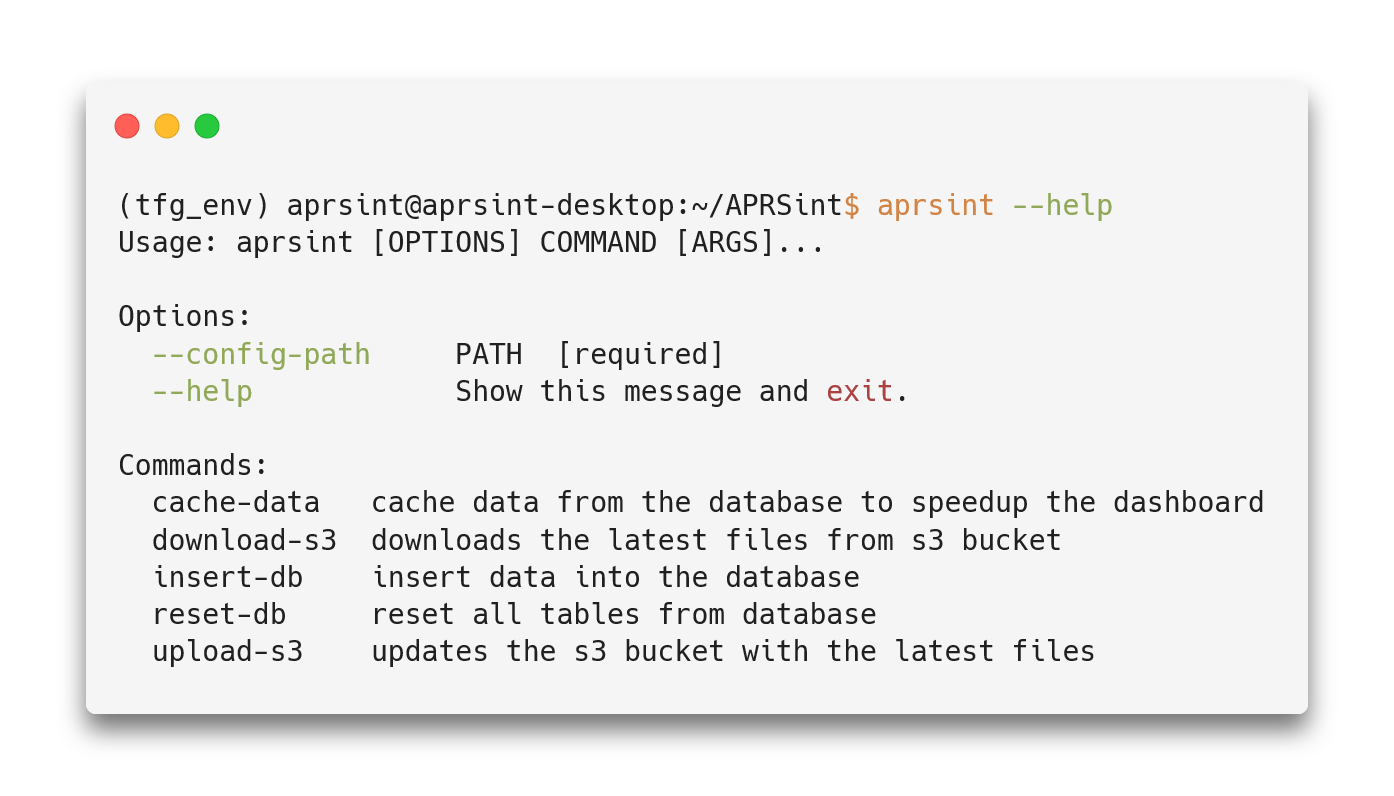
\includegraphics[width=0.85\textwidth]{Imagenes/Chapter_4/click_help.png}
	\caption[Ejemplo de uso de Click.]{Ejemplo de uso de Click (elaboración propia).}
	\label{fig:click-example}
\end{figure}

\subsection{Apache Airflow}
Apache Airflow es una plataforma de orquestación de tareas y flujos de trabajo. Es similar a Cron de Unix, pero permite una mayor personalización y control de las tareas que ejecuta. Las tareas se definen en archivos separados facilitando la compartimentalización y ofreciendo una mayor robustez y escalabilidad.
\begin{itemize}
	\item \textbf{Orquestación de flujos de trabajo:} Airflow facilita la orquestación de flujos de trabajo complejos al permitir definir tareas y sus dependencias como DAG's, lo que proporciona una visión clara de la lógica de ejecución.
	\item \textbf{Escalabilidad:} Airflow es altamente escalable y puede manejar flujos de trabajo de cualquier tamaño, desde tareas simples hasta flujos de trabajo altamente complejos.
	\item \textbf{Monitorización y alertas:} Proporciona una interfaz de usuario web para monitorizar el estado de los flujos de trabajo, así como capacidades de alerta para detectar y responder a fallos o retrasos en la ejecución de tareas.
	\item \textbf{Extensibilidad:} Airflow es altamente extensible y permite integrar fácilmente con otros sistemas y herramientas, lo que permite construir flujos de trabajo personalizados que se adapten a las necesidades específicas del proyecto.
\end{itemize}

\subsection{Configuración del proyecto}

Para la configuración del proyecto se ha utilizado un entorno virtual de Conda. Se ha creado un entorno virtual con las librerías necesarias para la ejecución de la aplicación. Algunas de las librerías más importantes que se han utilizado son las siguientes:

\begin{itemize}
	\item \textbf{Aprslib:} Para la recepción y decodificación de paquetes APRS.
	\item \textbf{Boto3:} Para la interacción con los servicios de AWS.
	\item \textbf{SQLAlchemy:} Para la interacción con la base de datos PostgreSQL.
	\item \textbf{Pandas:} Para la compresión y descompresión de ficheros.
	\item \textbf{Dash:} Para la creación de la aplicación web interactiva.
	\item \textbf{Click:} Para la creación de herramientas de línea de comandos.
\end{itemize}

Se ha creado un archivo de configuración en el que se definen las variables de entorno necesarias para la ejecución de la aplicación. Estas variables incluyen la configuración de la base de datos, las credenciales de AWS y la configuración de la aplicación web, entre otras.

Adicionalmente se ha configurado el proyecto con setuptools para facilitar la instalación y distribución de la aplicación. Se ha creado un archivo setup.py en el que se definen las dependencias del proyecto y se especifica la estructura del proyecto. Esto permite instalar la aplicación con un simple comando de pip.

$$pip\ install\ -i\ .$$

\section{Adquisición de datos}
En esta sección se describirá con detalle el módulo de adquisición de datos de la aplicación, incluyendo la arquitectura, los componentes y las tecnologías utilizadas.

\subsection{RTL-SDR}
En la primera fase del proyecto se adquirió un \textit{dongle} RTL-SDR con el fin de recibir los paquetes APRS y procesarlos posteriormente. Estos dongles son relativamente baratos oscilando entre los 30 y 100 euros, se conectan mediante usb al ordenador y disponen de un puerto SMA en la parte superior para la antena. La peculiaridad de estos dispositivos reside en que son controlables mediante \textit{software} y se pueden sintonizar en un rango de frecuencias muy amplio (24MHz a 1.7GHz).

Para utilizar estos dispositivos se necesita \textit{software} especializado como GQRX, CubicSDR o SDRSharp. Es posible también usar RTL-SDR en la terminal creando un micrófono virtual para que el \textit{software} de análisis pueda decodificar los paquetes.

Tras multitud de pruebas fallidas con distintos \textit{software} de visualización y análisis y \textit{software} de audio como Direwolf, se decidió no continuar por ese camino y probar otras alternativas como la que finalmente se ha implementado y se explica en la siguiente sección.

\subsection{APRS-IS}
APRS-IS es un sistema que permite la transmisión de mensajes APRS por Internet. La ventaja principal de este sistema, en comparación con la recopilación de información mediante una antena, es que permite obtener un flujo de datos mucho mayor. Esto se debe a la extensa red de antenas distribuidas globalmente. Además, otra ventaja significativa es la capacidad de recibir datos de cualquier parte del mundo sin necesidad de tener una antena en esa ubicación.

\subsubsection*{Infraestructura de la red APRS-IS}
Componentes principales:
\begin{itemize}
	\item \textbf{Trackers o TNC:} Son los emisores de los paquetes APRS, suelen corresponder a estaciones fijas o móviles que envían por radio los paquetes con información de posición, velocidad, rumbo, etc.
	\item \textbf{Digipeaters:} Son estaciones que reciben los paquetes APRS y los retransmiten, permitiendo que los paquetes lleguen a una mayor distancia. Son análogos a los repetidores de internet.
	\item \textbf{I-Gates:} Son estaciones que reciben los paquetes APRS por radio y los envían a la red APRS-IS, permitiendo que los paquetes sean accesibles a través de internet.
	\item \textbf{Servidores APRS-IS:} Son servidores que reciben los paquetes APRS de los I-Gates y los almacenan en una base de datos, permitiendo que los clientes accedan a los paquetes a través de internet. Los servidores APRS-IS suelen estar distribuidos geográficamente para mejorar la disponibilidad y la redundancia.
	\item \textbf{Clientes APRS-IS:} Pueden ser otros servidores, aplicaciones web o aplicaciones móviles que acceden a los servidores APRS-IS para obtener los paquetes APRS y mostrarlos a los usuarios.
\end{itemize}

La ruta que sigue un paquete APRS desde un tracker hasta un cliente APRS-IS se visualiza en la \Cref{fig:aprs-infra} y comprende los siguientes pasos: primero, un dispositivo \textbf{tracker} emite un paquete APRS a través de radiofrecuencia. Este paquete es recibido por un \textbf{Digipeater}, que funciona como un repetidor y retransmite la señal. Luego, un \textbf{I-Gate} recoge el paquete y lo envía a un servidor \textbf{APRS-IS} a través de Internet. Por último, un \textbf{cliente} APRS-IS accede a este servidor para recuperar el paquete y presentarlo al usuario para su visualización.

\begin{figure}[!h]
	\centering
	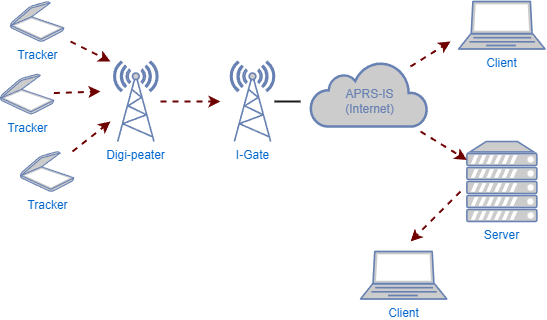
\includegraphics[width=0.95\textwidth]{Imagenes/Chapter_4/aprs_infra.png}
	\caption[Infraestructura de la red APRS - APRS-IS.]{Infraestructura de la red APRS - APRS-IS (elaboración propia).}
	\label{fig:aprs-infra}
\end{figure}

\FloatBarrier

Se ha seleccionado APRS-IS como fuente de datos para la aplicación debido a su facilidad de uso, su disponibilidad y la gran cantidad de información que ofrece desde sus servidores.

\subsection{La trama APRS}
El sistema APRS utiliza tramas AX.25 (Amateur X.25) para la transmisión de datos a través de las ondas de radio. El protocolo X.25 es un protocolo de nivel de enlace de datos que se diseñó y se creó para redes de conmutación de paquetes. El protocolo AX.25 es una versión simplificada del protocolo X.25 que se utiliza en las redes de radioaficionados.

\subsubsection*{Formato de la Trama APRS}

Todos los paquetes APRS se envían utilizando tramas \textbf{no numeradas} a diferencia de otros protocolos como TCP que utilizan tramas numeradas. Se muestra un ejemplo de trama APRS en la \Cref{fig:aprs-frame}.

\begin{figure}[h]
	\centering
	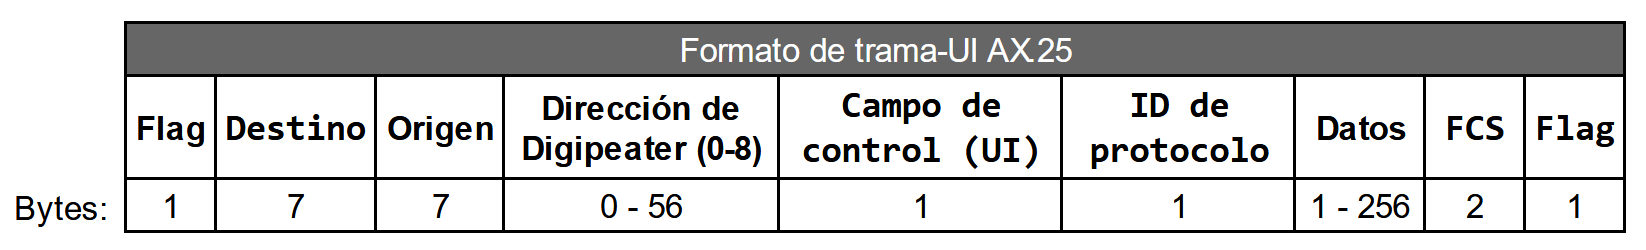
\includegraphics[width=1\textwidth]{Imagenes/Chapter_4/AX.25Frame.png}
	\caption[Formato de trama AX.25.]{Formato de trama AX.25 (elaboración propia, \cite{APRSProtocol}).}
	\label{fig:aprs-frame}
\end{figure}

Una trama AX.25 consta de los siguientes campos:
\begin{itemize}
	\item \textbf{Flag:} Marca el inicio y el final de la trama. Tiene un valor fijo de 0x7E.
	\item \textbf{Destino:} Identifica la estación de destino de la trama. Puede ser una dirección de estación completa o una dirección abreviada.
	\item \textbf{Origen:} Identifica la estación de origen de la trama. Puede ser una dirección de estación completa o una dirección abreviada.
	\item \textbf{Dirección de Digipeater (0-8):} Identifica los repetidores que deben reenviar la trama. Puede haber hasta 8 repetidores en la ruta.
	\item \textbf{Campo de control (UI):} Este campo se establece a 0x03 (trama no numerada).
	\item \textbf{ID de protocolo:} Este campo se establece a 0xF0 (no hay protocolo de capa 3).
	\item \textbf{Datos:} Este campo contiene los datos de la trama. En el caso de las tramas APRS, este campo puede contener información sobre la posición, la velocidad, el estado y otros datos de la estación.
	\item \textbf{FCS:} Frame Check Sequence (FCS): Es un código de verificación de redundancia cíclico (CRC) que se utiliza comprobar la integridad de la trama.
\end{itemize}


\subsubsection*{Contenido de la Trama}

Dentro del campo de datos de una trama AX.25, se pueden incluir diversos datos relevantes para APRS. Esto puede incluir información de posición (latitud y longitud), velocidad, altitud, rumbo, comentarios del operador, mensajes de texto, etc \ldots \cite{APRSPaths}\cite{APRS}.

\[\underbrace{\textbf{\textcolor{red}{NOCALL}}}_{Origen}>\underbrace{\textbf{\textcolor[HTML]{FA9F42}{APRS}}}_{Destino}, \underbrace{\textbf{\textcolor{blue}{OH7RDA,OH7RDB}}}_{Digipeaters\ y\ I-Gates}:\underbrace{\textbf{\textcolor{green}{!4903N07201W-test A=001234}}}_{Mensaje}\]

En este ejemplo, el campo de datos contiene información sobre posición, altitud y un comentario. La posición está representada en formato APRS, que es una forma abreviada de representar la latitud y longitud en grados decimales. La altitud se representa en pies y el comentario es un mensaje de texto opcional, en este caso es \textit{``test''}.

\subsubsection*{Uso en APRS}

En el contexto de APRS, las tramas AX.25 se utilizan para transmitir actualizaciones de posición de estaciones móviles, estaciones meteorológicas, balizas y otros objetos de interés. Estas tramas son recibidas por otras estaciones en la red APRS, lo que permite el seguimiento en tiempo real de la ubicación y otros datos de interés.

\subsection{Recepción de paquetes APRS}

Para la recepción de paquetes APRS se ha utilizado la librería Aprslib de Python. Esta librería permite conectarse a un servidor APRS-IS y recibir los paquetes APRS en tiempo real. Se ha creado un sistema que utilizando esta librería se conecta a un servidor APRS-IS, recibe los paquetes APRS y los guarda en un \textit{buffer} en memoria. Cuando el \textit{buffer} se llena con aproximadamente 10.000 mensajes en alrededor de 15 segundos, se procede a escribir el \textit{buffer} en un fichero comprimido en el disco duro SSD.

Un detalle interesante es que los mensajes APRS no se decodifican en este punto, de hecho se guardan sin ningún tipo de procesamiento en ficheros binarios comprimidos en formato gzip para no ocupar mucho espacio en disco. Esto se hace así para evitar la sobrecarga de procesamiento en la Raspberry Pi y para poder procesar los mensajes en un servidor más potente en la nube.

Es importante mencionar que el sistema de recepción de paquetes APRS se ejecuta en segundo plano en modo demonio utilizando el gestor de procesos Supervisord, lo que garantiza que el sistema se mantenga en funcionamiento incluso en caso de fallos o reinicios del sistema.

\subsection{Procesado de paquetes APRS}
En esta sección se describirá con detalle el módulo de procesado de paquetes APRS de la aplicación, incluyendo la arquitectura, los componentes y las tecnologías utilizadas.

\subsubsection*{Subida de ficheros a AWS S3}

Una vez los ficheros se han guardado en el disco duro SSD, se procede a subirlos a un \textit{bucket} S3 en AWS. Para ello se ha utilizado la librería Boto3 de Python, que permite interactuar con los servicios de AWS desde Python. Se ha creado un \textit{script} que se ejecuta una vez al día mediante la orquestación de Apache Airflow y que sube los ficheros comprimidos al \textit{bucket} S3. Una vez subidos los ficheros, se eliminan del disco duro SSD para liberar espacio. Cuando un fichero se sube sube a S3 se desencadena un evento.

\subsubsection*{Procesado de paquetes APRS en AWS Lambda}

Una vez los ficheros se han subido a S3, se desencadena un evento que ejecuta una función lambda \Cref{fig:aws-lambda} en AWS. Esta función lambda se encarga de descomprimir el fichero, procesar los mensajes APRS y convertirlos en formato JSON.

Por defecto Lambda no puede hacer uso de librerías de terceros por lo que se ha tenido que encapsular la librería Aprslib en un fichero .zip, subirlo a Lambda y establecerlo como una capa de Lambda para poder hacer uso de ella.

Para la descompresión de los ficheros se ha utilizado la librería gzip de Python, que permite leer y escribir ficheros comprimidos en formato gzip.
Para el procesado de los mensajes APRS se ha utilizado la librería Aprslib de Python como ya hemos mencionado, que permite decodificar los mensajes APRS y extraer información útil como la posición, velocidad y rumbo de los objetos rastreados en formato clave-valor.


\noindent Esta función lambda se ejecuta de manera asíncrona y paralela, lo que permite procesar grandes volúmenes de mensajes APRS de manera eficiente y escalable. Una vez procesados los mensajes APRS, se eliminan los ficheros comprimidos del S3 de entrada (aprsinput) para liberar espacio y evitar duplicados.

Finalmente los mensajes procesados se guardan en un \textit{bucket} S3 de salida (aprsoutput) en formato JSON para su posterior descarga. La descarga de los ficheros JSON ocurre una vez al día mediante la orquestación de Apache Airflow y la librería Boto3. Estos ficheros (uno por fichero de entrada) se descargan a otra carpeta temporal en la Raspberry Pi.

\begin{figure}[h]
	\centering
	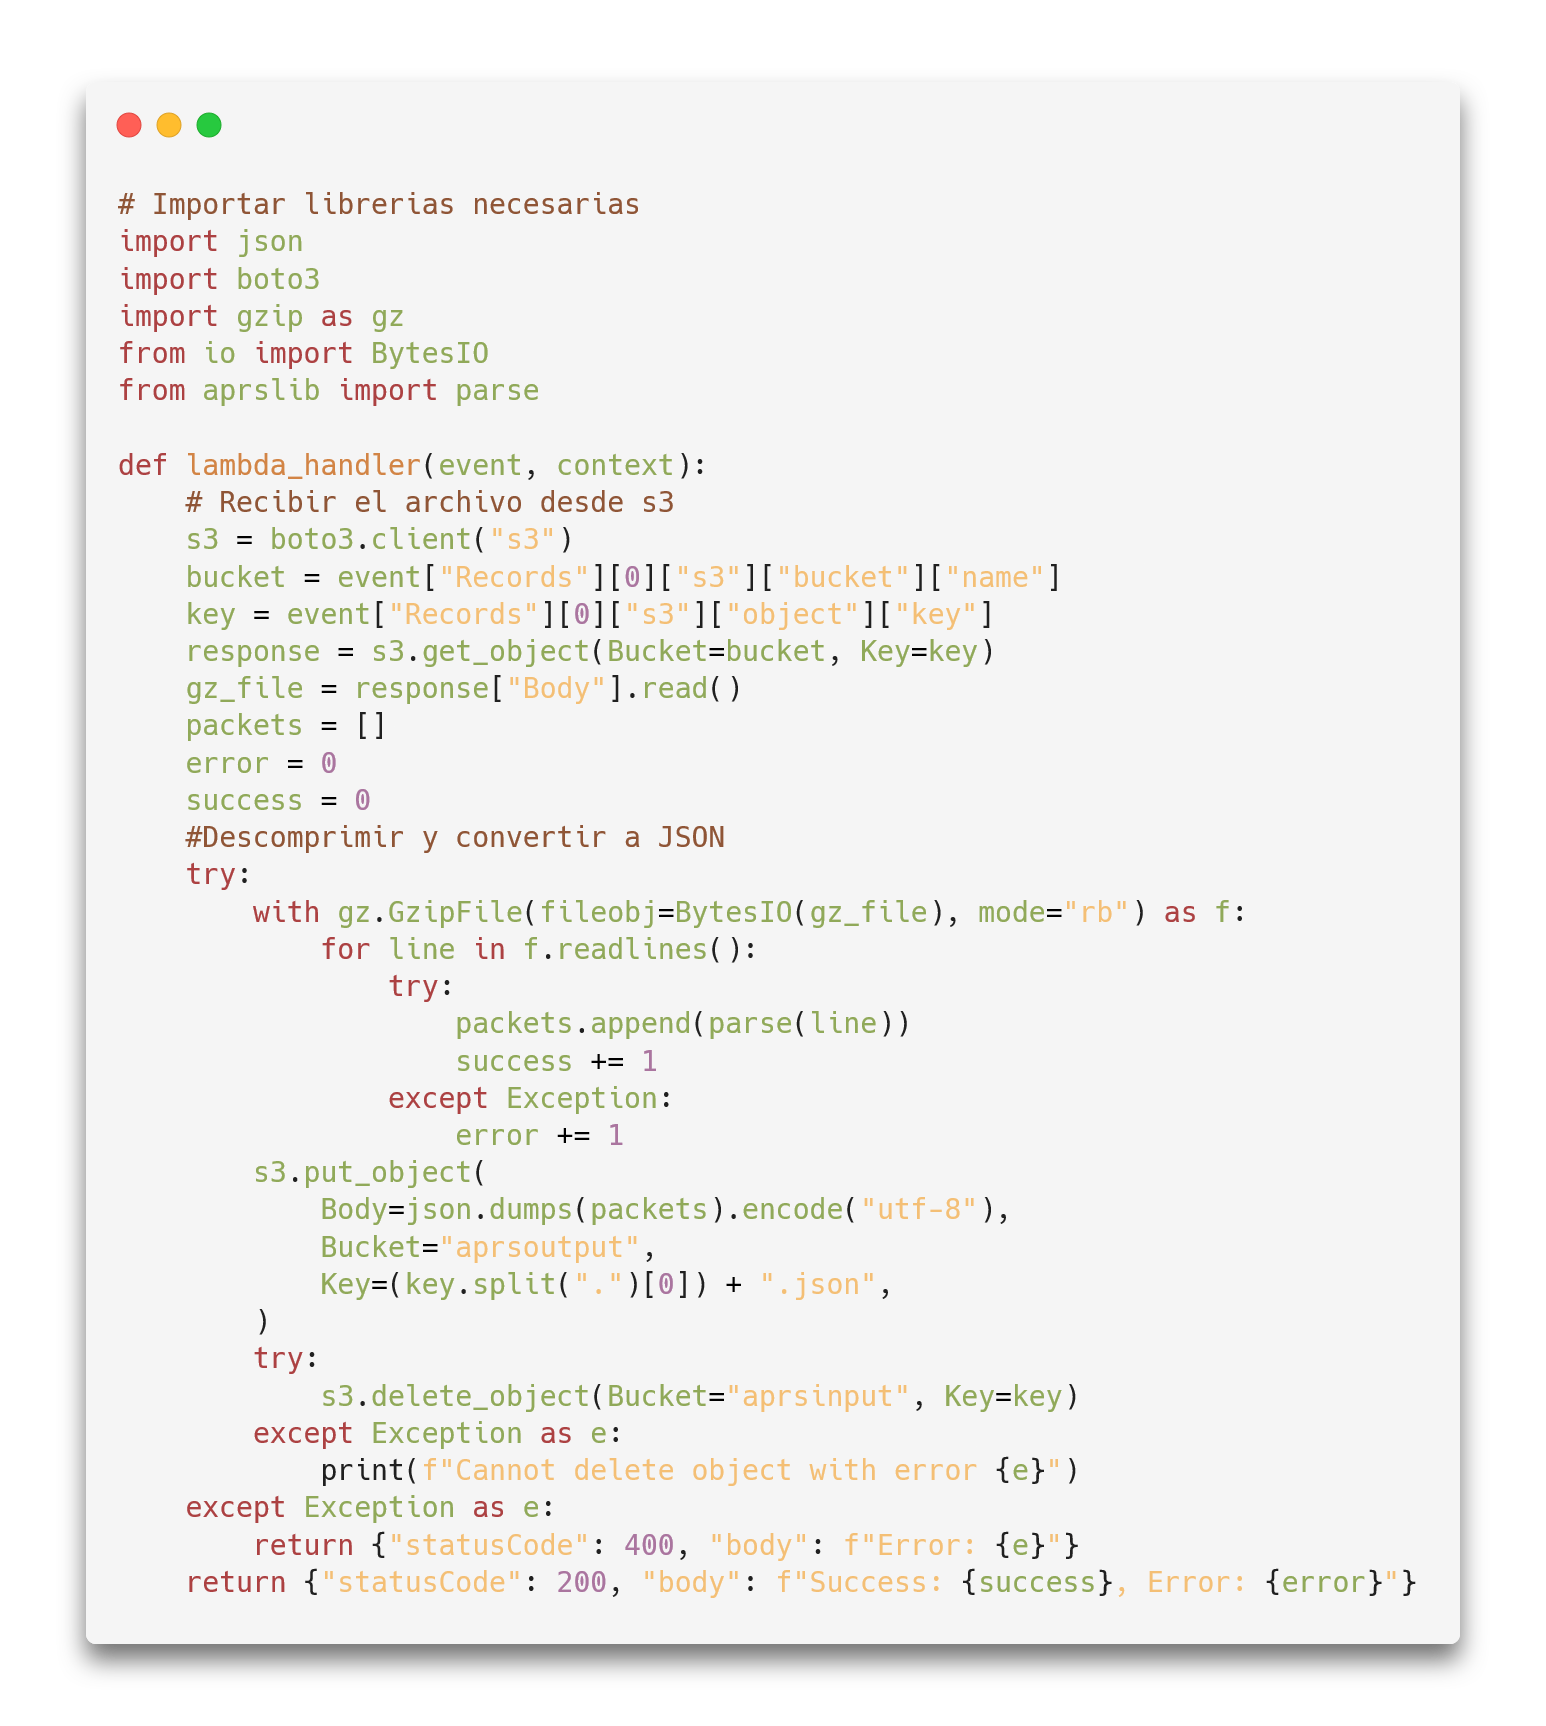
\includegraphics[width=0.8\textwidth]{Imagenes/Chapter_4/lambda.png}
	\caption[Procesado de paquetes APRS en AWS Lambda.]{Procesado de paquetes APRS en AWS Lambda (elaboración propia).}
	\label{fig:aws-lambda}
\end{figure}

\subsection{Almacenamiento de paquetes en la base de datos}

Una vez los ficheros JSON ya procesados se han descargado al directorio temporal en la Raspberry Pi, se procede a almacenarlos en la base de datos PostgreSQL. Para ello se ha utilizado la librería SQLAlchemy de Python, que permite interactuar con bases de datos relacionales de manera sencilla y eficiente. Se ha creado un \textit{script} que se ejecuta una vez al día mediante la orquestación de Apache Airflow y que lee los ficheros JSON, procesa los mensajes APRS y los almacena en la base de datos.

Este paso esconde un gran problema que hubo de ser solucionado. El \textit{script} en un principio seguía los siguientes pasos.

\begin{enumerate}
	\item \textbf{Lectura de ficheros JSON:} El \textit{script} lee los ficheros JSON de la carpeta local /tmp descargados del \textit{bucket} S3.
	\item \textbf{Extracción de la estación:} El \textit{script} extrae la estación origen y destino de cada mensaje y en caso de no existir en la base de datos las crea.
	\item \textbf{Extracción de las posiciones:} Se extraen las posiciones (si las hay) de cada mensaje y el timestamp si lo hay y se almacenan en la base de datos.
	\item \textbf{Identificación del país:} Mediante la librería Geopy y ficheros de formas de países se identifica el país de la estación.
	\item \textbf{Extracción de los mensajes:} Se extraen los mensajes de cada línea del JSON y se almacenan en la base de datos.
\end{enumerate}

\noindent Al utilizar este enfoque, se detectó un gran problema de rendimiento, ya que cada archivo JSON contenía alrededor de 10.000 mensajes y en la creación de los objetos, inserciones en la BD y detección del país se tardaba alrededor de 40 segundos por fichero JSON. Esto aunque no parezca demasiado tiempo, si se tiene en cuenta que la cantidad de mensajes APRS que se reciben en 40 segundos es alrededor de 45.000, se puede ver que el sistema no era escalable.

\subsubsection*{\underline{Optimizaciones}}
Para solucionar este problema se realizaron las siguientes optimizaciones:
\begin{itemize}
	\item \textbf{Uso de sets:} Se ha cambiado el uso de consultas a la BD por sets en la creación de las estaciones para acelerar la comprobación la existencia de una estación en la base de datos.
	\item \textbf{Inserción por lotes:} Se ha modificado la interfaz con SQLAlchemy para permitir inserciones en lotes de 250 mensajes.
	\item \textbf{Detección de países:} Se ha cambiado la librería Geopy por GeoPandas que permite la una detección de países más rápida utilizando paralelización.
\end{itemize}
Estas optimizaciones han acelerado el tiempo de procesado de un fichero JSON de 40 a 2 segundos, lo que ha permitido que el sistema sea escalable y pueda procesar grandes volúmenes de mensajes de manera eficiente.

\subsection{Base de datos}
Como se ha mencionado previamente, se ha elegido PostgreSQL como sistema de gestión de bases de datos para la aplicación. Esta elección se ha basado en la robustez, la fiabilidad y la capacidad de manejar grandes volúmenes de datos que ofrece PostgreSQL incluso en sistemas con recursos reducidos. La base de datos se ha diseñado siguiendo un modelo relacional \Cref{fig:db-model} que permite almacenar y relacionar la información de los mensajes APRS de manera eficiente, el modelo cuenta con las siguientes tablas.

\begin{itemize}
	\item \textbf{stations:} Almacena la información de las estaciones APRS, incluyendo el identificador de la estación (CALLSIGN), el ssid y su símbolo en formato caracter.
	\item \textbf{station\textunderscore locations:} Almacena la información de las posiciones \footnote[1]{Esta tabla tiene un campo id en la clave primaria por si una estación ha emitido un mensaje sin timestamp} de las estaciones APRS, incluyendo el país, la latitud, la longitud y la fecha y hora en la que se han recibido.
	\item \textbf{messages:} Almacena la información de los mensajes APRS, incluyendo el contenido del mensaje, el tipo de mensaje, el timestamp y el mensaje original retransmitido.
	\item \textbf{qrz\textunderscore profiles:} Sirve como una caché que almacena la información de los perfiles de los usuarios de QRZ, incluyendo el identificador (CALLSIGN), el nombre, la dirección, la ciudad, el estado, el código postal, el país, la latitud, la longitud y la fecha de nacimiento entre muchos otros.
\end{itemize}

\begin{figure}[h]
	\centering
	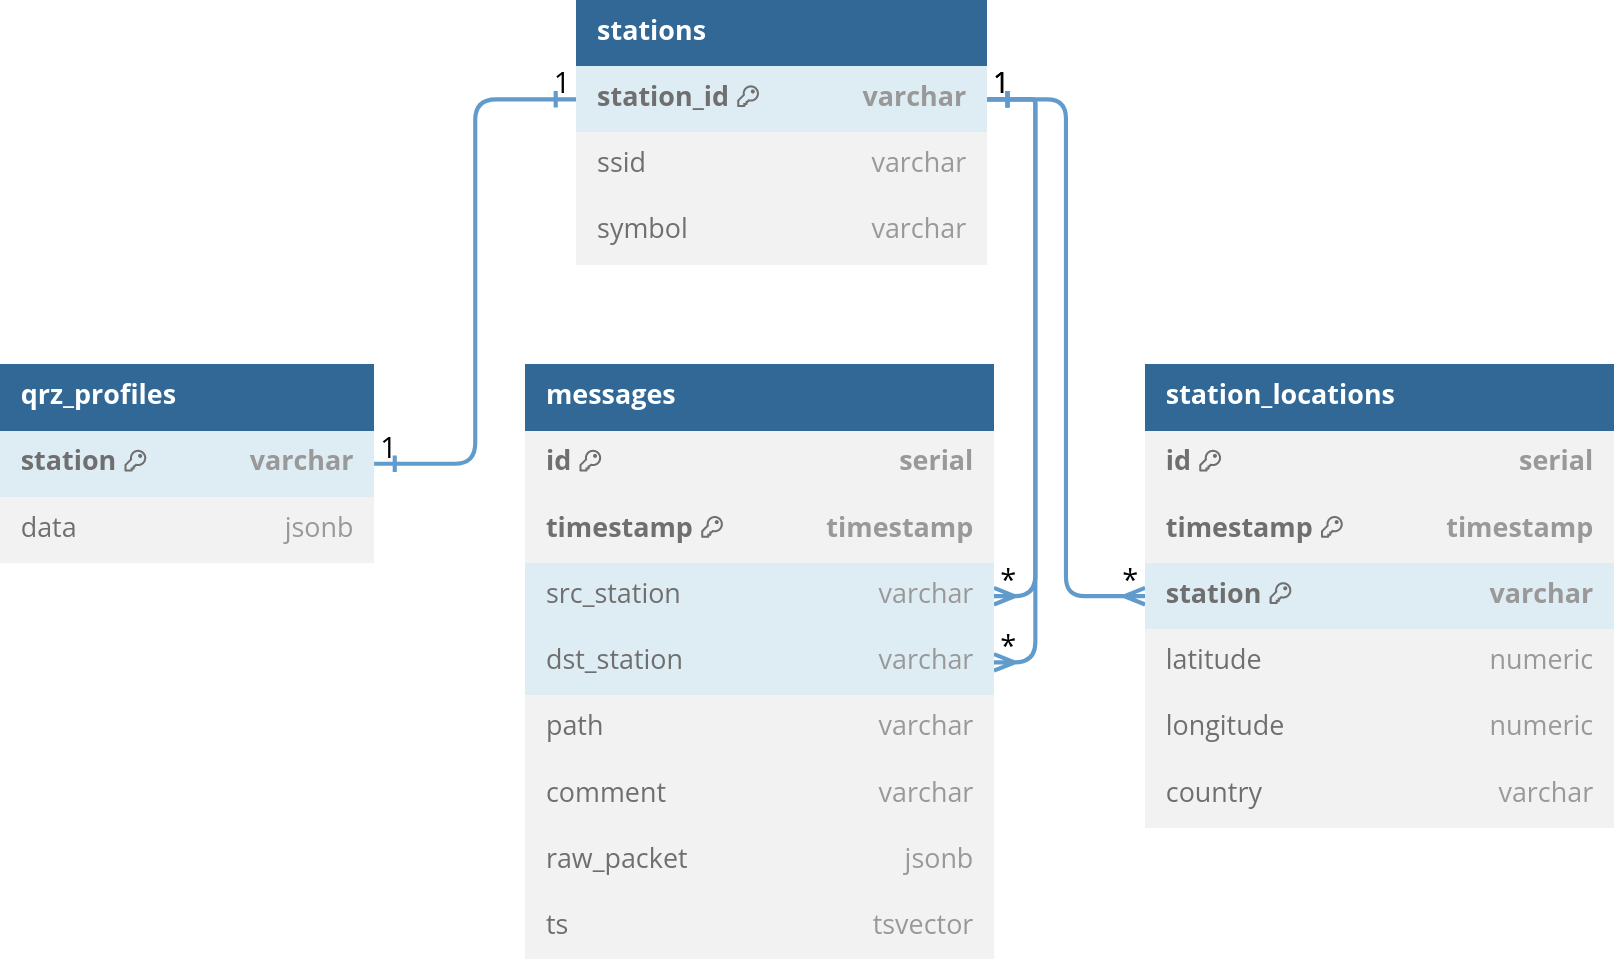
\includegraphics[width=0.9\textwidth]{Imagenes/Chapter_4/db_diagram.png}
	\caption[Estructura de la base de datos.]{Estructura de la base de datos (elaboración propia).}
	\label{fig:db-model}
\end{figure}

\FloatBarrier

\subsection{Flujo de un paquete APRS}
En esta sección se describe con detalle el flujo de un paquete APRS a través de la aplicación, desde la recepción hasta el almacenamiento en la base de datos.
\begin{enumerate}
	\item \textbf{Recepción:} El paquete APRS se recibe a través de la red APRS-IS y se almacena en un \textit{buffer} en memoria.
	\item \textbf{Almacenamiento en disco:} Cuando el \textit{buffer} se llena con aproximadamente 10.000 mensajes, se escribe el \textit{buffer} en un fichero comprimido en el disco duro SSD.
	\item \textbf{Subida a S3:} El fichero comprimido se sube a un \textit{bucket} S3 en AWS para su procesamiento posterior.
	\item \textbf{Procesado en Lambda:} Una función lambda en AWS descomprime el fichero, procesa los mensajes APRS y los convierte en formato JSON.
	\item \textbf{Almacenamiento en S3:} Los ficheros JSON procesados se guardan en un \textit{bucket} S3 de salida para su posterior descarga.
	\item \textbf{Descarga a la Raspberry Pi:} Una vez al día, los ficheros JSON se descargan a una carpeta temporal en la Raspberry Pi.
	\item \textbf{Almacenamiento en la base de datos:} Un \textit{script} en la Raspberry Pi lee los ficheros JSON, procesa los mensajes APRS y los almacena en la base de datos PostgreSQL.
\end{enumerate}

\begin{figure}[h]
	\centering
	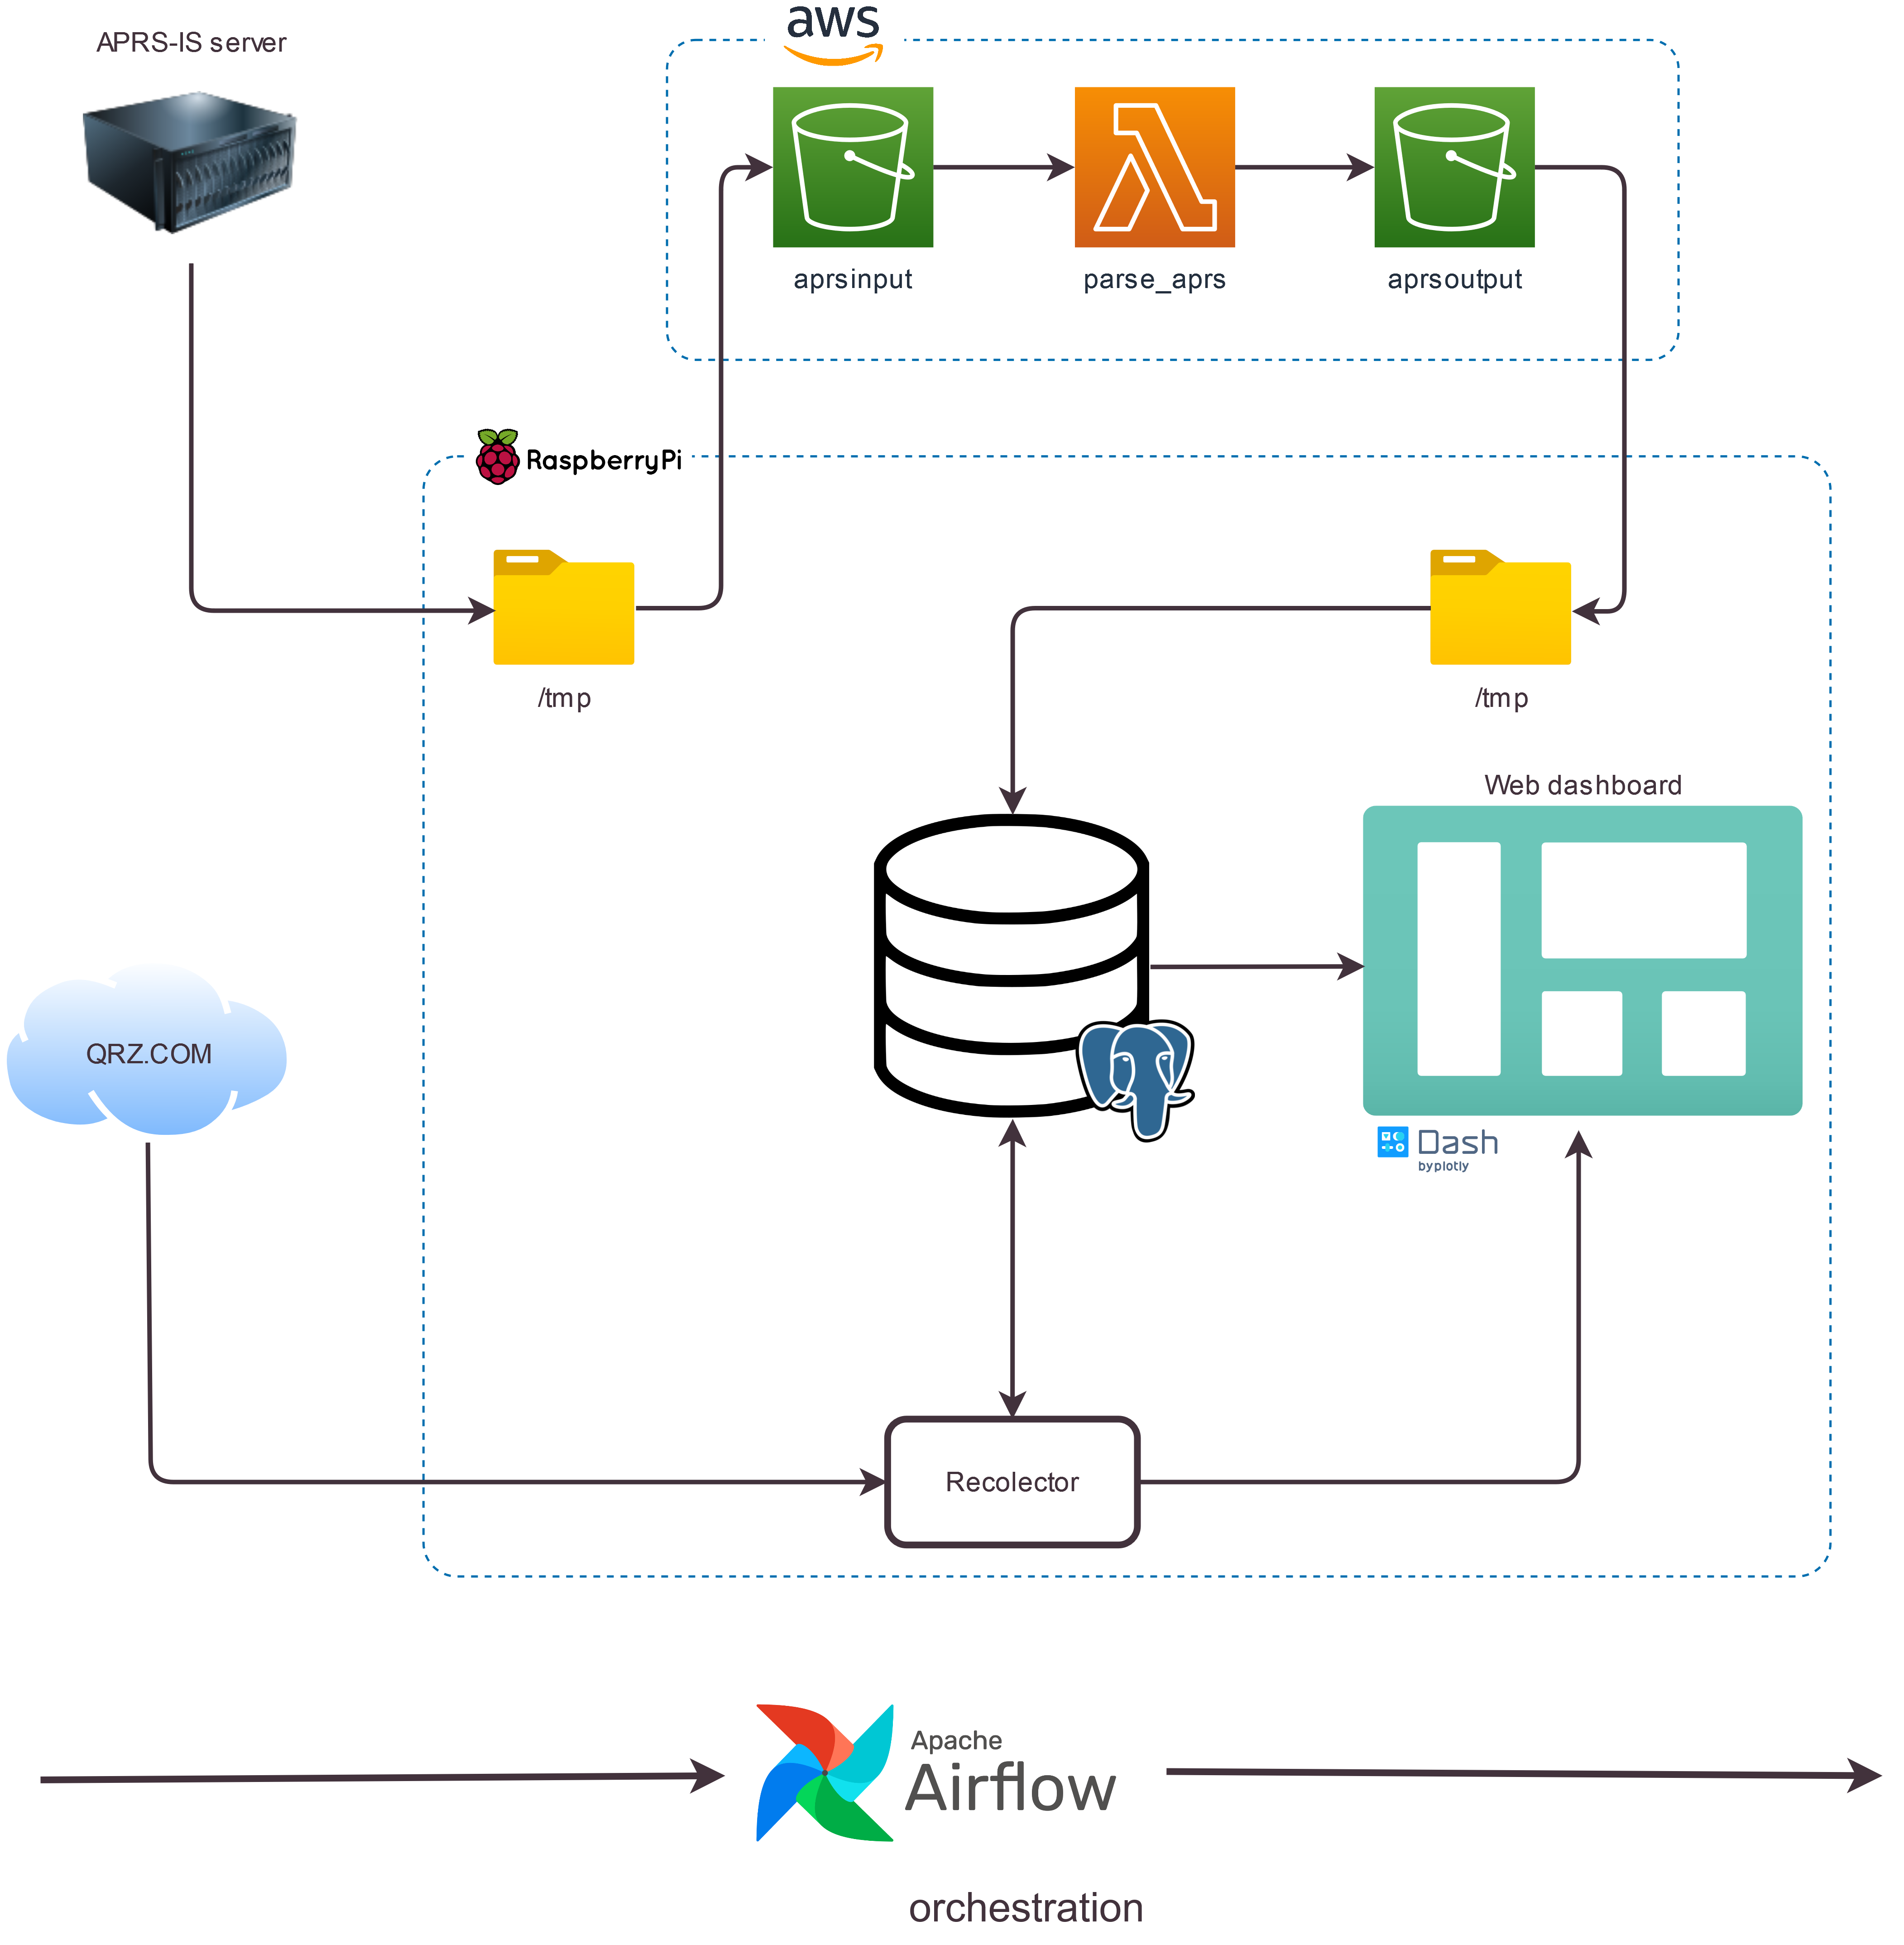
\includegraphics[width=0.8\textwidth]{Imagenes/Chapter_4/cloud_arch.png}
	\caption[Flujo de datos en APRSINT.]{Flujo de datos en APRSINT (elaboración propia).}
	\label{fig:aws-s3}
\end{figure}

\section{Visualización y presentación de datos}

En esta sección se describe con detalle el módulo de visualización y presentación de datos de la aplicación, incluyendo la arquitectura, los componentes y las tecnologías utilizadas.

\subsection{Dash}
Dash es un \textit{framework} de Python creado por Plotly para la creación de aplicaciones web interactivas y visualizaciones de datos. Dash permite crear aplicaciones web interactivas y visualizaciones de datos atractivas utilizando Python como lenguaje de programación. Dash está escrito encima de Plotly.js, React y Flask lo que permite una gran capacidad de personalización.

Dash ofrece una versión de pago llamada Dash Enterprise que ofrece una gran cantidad de funcionalidades para elaborar aplicaciones web de manera más rápida y sencilla. Sin embargo, para este proyecto se ha utilizado la versión gratuita de Dash, con algunas librerías adicionales entre las que se encuentran:

\begin{itemize}
	\item \textbf{Dash core components:} Contiene multitud de componentes interactivos como gráficos, tablas, \textit{sliders}, \textit{dropdowns}, entre otros, que permiten a los usuarios interactuar con los datos de manera intuitiva.
	\item \textbf{Dash html components:} Contiene los \textit{wrappers} de las etiquetas HTML como \textit{divs}, \textit{spans}, \textit{inputs}, entre otros, que permiten personalizar la apariencia y el diseño de la aplicación web.
	\item \textbf{Dash mantine components:} Ofrece una amplia gama de componentes de Mantine como \textit{navbars}, tarjetas, modales, entre otros, que permiten crear aplicaciones web atractivas y responsivas.
	\item \textbf{Dash express:} Añade componentes extra como un panel de filtrado y una barra de navegación \footnote{Se ha modificado esta librería para adaptarla a la estructura de la aplicación.}.
	\item \textbf{Plotly express:} Es el principal competidor de Matplotlib en el mundo de la visualización de datos en Python. Ofrece una gran cantidad de gráficos y visualizaciones de datos interactivos.
\end{itemize}

\subsection{Diseño}
El diseño de la aplicación web se ha basado en la simplicidad, la usabilidad y la accesibilidad. El primer diseño del proyecto se realizó en la aplicación de prototipado Figma como se muestra en la \Cref{fig:figma}.

\begin{figure}[h]
	\centering
	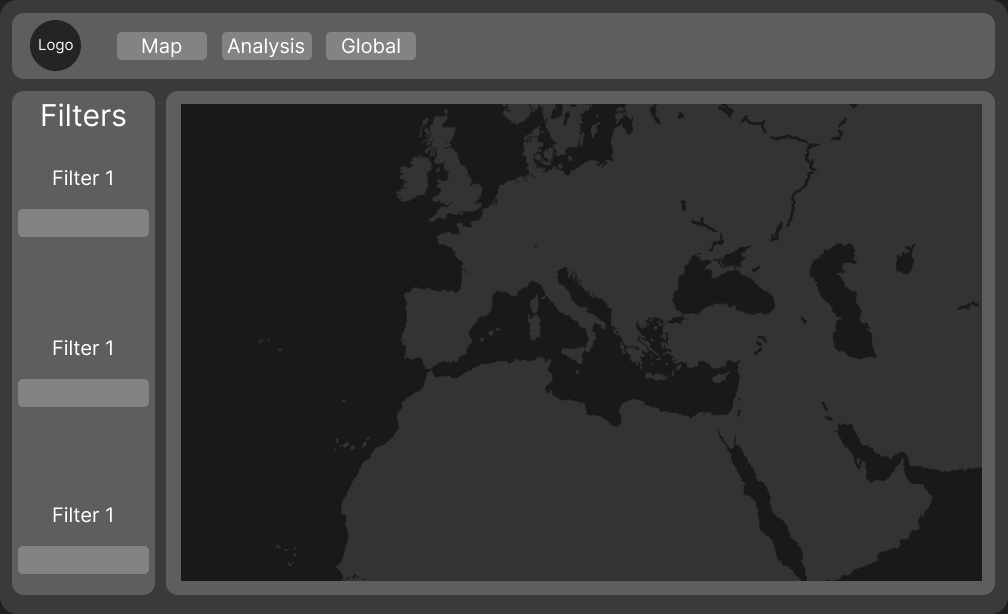
\includegraphics[width=0.8\textwidth]{Imagenes/Chapter_4/first_draft.png}
	\caption[Primer diseño de la aplicación web en Figma.]{Primer diseño de la aplicación web en Figma (elaboración propia).}
	\label{fig:figma}
\end{figure}

\noindent Este diseño se ha ido modificando y adaptando a lo largo del desarrollo del proyecto para mejorar la usabilidad y la experiencia del usuario. Este diseño muestra la pantalla principal de la aplicación, que incluye un mapa con las estaciones APRS, y un panel de control con filtros y opciones de visualización.

\subsection{Home - Primera pantalla}
En esta sección se describe la primera pantalla de la aplicación web, que muestra un mapa con las estaciones APRS y un panel de control con filtros y opciones de visualización.

\subsubsection*{Obtención de datos}

Siguiendo la estrategia de otros sistemas de \textit{dashboarding} como PowerBI o Tableau y con el objetivo de mejorar la eficiencia y la escalabilidad del sistema, se ha optado por eliminar en lo posible las consultas a la base de datos en tiempo real. Para ello se ha creado un sistema de caché que almacena los datos a representar en esta pantalla en un archivo de rápida lectura que es actualizado diariamente mediante Apache Airflow. Este sistema de caché permite reducir la carga en la base de datos y mejorar el rendimiento de la aplicación web.

El sistema de caché se ha implementado utilizando la librería Pandas de Python, usando un fichero .feather para almacenar los datos en formato binario y comprimido y reducir significativamente\footnote{Los ficheros de tipo .feather son hasta 100 veces más rápidos en lectura y escritura que los ficheros .csv\cite{CsvVsFeather}} el tiempo de carga de la página.

\subsubsection*{Mapa de estaciones APRS}

El mapa de estaciones APRS muestra la posición de cada una de las estaciones APRS, representadas por un marcador en el mapa. Es un mapa interactivo que permite hacer zoom, desplazarse y al posicionar el cursor encima de una estación aparecerá un recuadro ofreciendo información adicional.

Esta página hace uso de la librería Plotly para renderizar el mapa y del servicio web de mapas Mapbox para obtener los mapas y estilos de mapa.

\subsubsection*{Filtros}
El panel de control de la aplicación web incluye una serie de filtros y opciones de visualización que permiten al usuario personalizar la información mostrada en el mapa. La ventaja de estos filtros es que son aditivos y se pueden combinar para obtener con exactitud la información requerida. Los filtros disponibles son:

\begin{itemize}
	\item \textbf{Filtro por rango de fechas:} Permite filtrar las estaciones APRS por rango de fechas, mostrando solo las estaciones de las que se ha recibido algún mensaje en el rango de fechas seleccionado.
	\item \textbf{Filtro por país:} Permite filtrar las estaciones APRS por país, mostrando solo las estaciones que se encuentran en el país seleccionado.
	\item \textbf{Filtro por contenido del mensaje:} Este es quizás el filtro más interesante, ya que permite filtrar las estaciones por el contenido del mensaje, este filtro será explicado más adelante.
	\item \textbf{Filtro por tipo de estación:} Permite filtrar las estaciones APRS por tipo, mostrando solo las estaciones que corresponden al tipo seleccionado.
	\item \textbf{Filtro por ssid:} Permite filtrar las estaciones por ssid.
\end{itemize}

\subsubsection*{Búsqueda difusa en contenido de mensajes}
Este filtro es personalmente el más interesante de todos los filtros disponibles. El objetivo es permitir al usuario buscar mensajes emitidos por las estaciones que contengan una palabra o frase especifica. Para ello se han probado varias alternativas como el uso de expresiones regulares o una implementación en Python puro. El problema de estas opciones es que son muy lentas para el enorme volumen de datos con el que se cuenta y al ser dinámico no era factible realizar esa búsqueda en tiempo real.

Finalmente se ha optado por el uso de PostgreSQL FTS (\textit{Full Text Search}). PostgreSQL FTS es un sistema de búsqueda de texto completo que permite realizar búsquedas de texto en grandes volúmenes de datos de manera eficiente. Las ventajas que ofrece este sistema son:

\begin{itemize}
	\item \textbf{Rendimiento:} Todo el proceso de búsqueda se realiza en la base de datos, lo que permite realizar búsquedas de texto sin transferir todos los mensajes al servidor para su búsqueda.
	\item \textbf{Búsqueda difusa:} Permite realizar búsquedas de texto difuso, lo que significa que se pueden buscar palabras o frases que contengan errores tipográficos o que no coincidan exactamente con el texto buscado.
	\item \textbf{Indexación:} PostgreSQL FTS indexa automáticamente los mensajes de texto, lo que permite realizar búsquedas de texto de manera eficiente incluso en grandes volúmenes de datos.
\end{itemize}

Se ha creado un índice de texto completo en la columna de mensajes de la tabla de mensajes y se ha utilizado la función to\textunderscore tsvector para convertir los mensajes en un vector de texto completo. Posteriormente se ha utilizado la función plainto\textunderscore tsquery para convertir la palabra o frase de búsqueda en una consulta de texto completo y finalmente se ha utilizado la función ts\textunderscore query para realizar la búsqueda de texto completo en la columna de mensajes. Este filtro permite al usuario buscar mensajes emitidos por las estaciones que contengan una palabra o frase específica, lo que facilita la identificación y el análisis de los mensajes relevantes \cite{PostgreSQLFTS}.

Cuando un usuario realiza una búsqueda de texto completo, se muestra un modal con la lista de todos los mensajes que contienen la palabra o frase de búsqueda, ordenados por relevancia haciendo uso de la función ts\textunderscore rank. Otra funcionalidad interesante es que la palabra o palabras buscadas se resaltan en el mensaje para facilitar su identificación como se muestra en la \Cref{fig:postgres-fts}.

\begin{figure}[h]
	\centering
	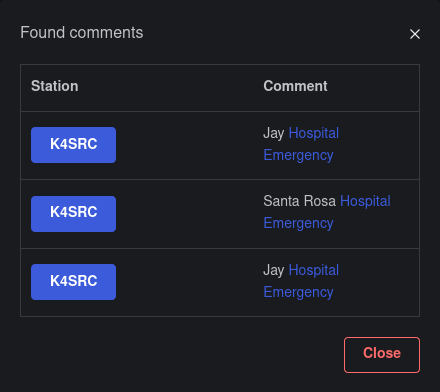
\includegraphics[width=0.5\textwidth]{Imagenes/Chapter_4/fts_output.png}
	\caption[Resultados de la búsqueda de <<emergency hospital>>.]{Resultados de la búsqueda de <<emergency hospital>> (elaboración propia).}
	\label{fig:postgres-fts}
\end{figure}

\noindent En el modal se muestra una tabla de dos columnas, la columna izquierda contiene un botón con el nombre de la estación y la columna derecha el contenido del mensaje.

\subsection{Station - Segunda pantalla}
Esta es la página que hace única a APRSINT. En esta página se muestra la información detallada de una estación APRS en concreto. Se puede llegar a esta pantalla desde la página principal haciendo clic en un marcador de una estación en el mapa, haciendo clic en una estación en la búsqueda en los mensajes o haciendo clic en un nodo del grafo de la página 3. La pantalla station está dividida en tres secciones.

\subsubsection*{Información de QRZ}
QRZ es una base de datos de radioaficionados que contiene información detallada sobre los radioaficionados de todo el mundo. Para acceder a la información disponible en la web de QRZ\footnote{\url{https://qrz.com}} es necesario tener una cuenta y estar registrado. QRZ cuenta con un servicio de API que permite acceder a la información de los radioaficionados de manera programática.

Para obtener la información de los radioaficionados se ha utilizado la librería requests de Python, que permite obtener la información necesaria de QRZ.

Con el fin de acelerar las consultas, se ha implementado una tabla en la base de datos para almacenar en caché las solicitudes, lo que disminuye la cantidad de consultas a una estación determinada si esta ya ha sido solicitada con anterioridad.

Este módulo es de los más complejos de la aplicación, pero a su vez de los más útiles, ya que permite al usuario obtener información muy detallada de una estación APRS en concreto y de la persona que está detrás. Algunos de los datos que se pueden obtener son:

\begin{itemize}
	\item Nombre de la persona registrada
	\item Fechas de registro y última actualización en la web
	\item Alias conocidos de la estación
	\item Dirección de la persona registrada (Como link a google maps)
	\item Fecha de nacimiento de la persona registrada
\end{itemize}

\subsubsection*{Información de posiciones}
Esta sección se compone de dos partes. En la parte superior se muestra un mapa con todas las posiciones reportadas por la estación, se muestra también la caja delimitadora de todas las posiciones.

En la parte inferior se muestran estadísticas de las posiciones reportadas por la estación como la frecuencia media de emisión, la primera y última emisión recibida y por cada mensaje emitido por la estación se muestra el número de repeticiones del mensaje y las URL (si existen) encontradas en los mensajes.

\subsubsection*{Información de mensajes}
Finalmente encontramos la sección de mensajes. En esta sección se muestra una tabla en la que se muestra la información de los mensajes emitidos por la estación. La tabla se compone de las siguientes columnas:
\begin{itemize}
	\item La fecha de emisión del mensaje.
	\item La latitud y longitud de la estación en el momento de la emisión.
	\item El país en el que se encontraba la estación en el momento de la emisión.
	\item La estación destino del mensaje.
	\item El \textit{path} es decir los \textit{Digipeaters} que han retransmitido el mensaje.
	\item El contenido del mensaje.
\end{itemize}

La tabla es interactiva y permite al usuario filtrar los mensajes por el intervalo de fechas que pretenda.

\subsection{Graph - Tercera pantalla}
Esta pantalla es la última de la web, en ella se muestra un grafo dirigido en el que los nodos son las estaciones y las aristas dirigidas, mensajes como se muestra en la \Cref{fig:graph}. El grafo es interactivo y permite hacer zoom, desplazarse y al posicionar el cursor encima de un nodo o arista aparecerá un recuadro ofreciendo información adicional. El color y tamaño de los nodos depende de la cantidad de mensajes que ha emitido o recibido la estación y de misma manera el color y tamaño de las aristas depende de la cantidad de mensajes que se han emitido o recibido desde la estación origen y destino.

\begin{figure}[h]
	\centering
	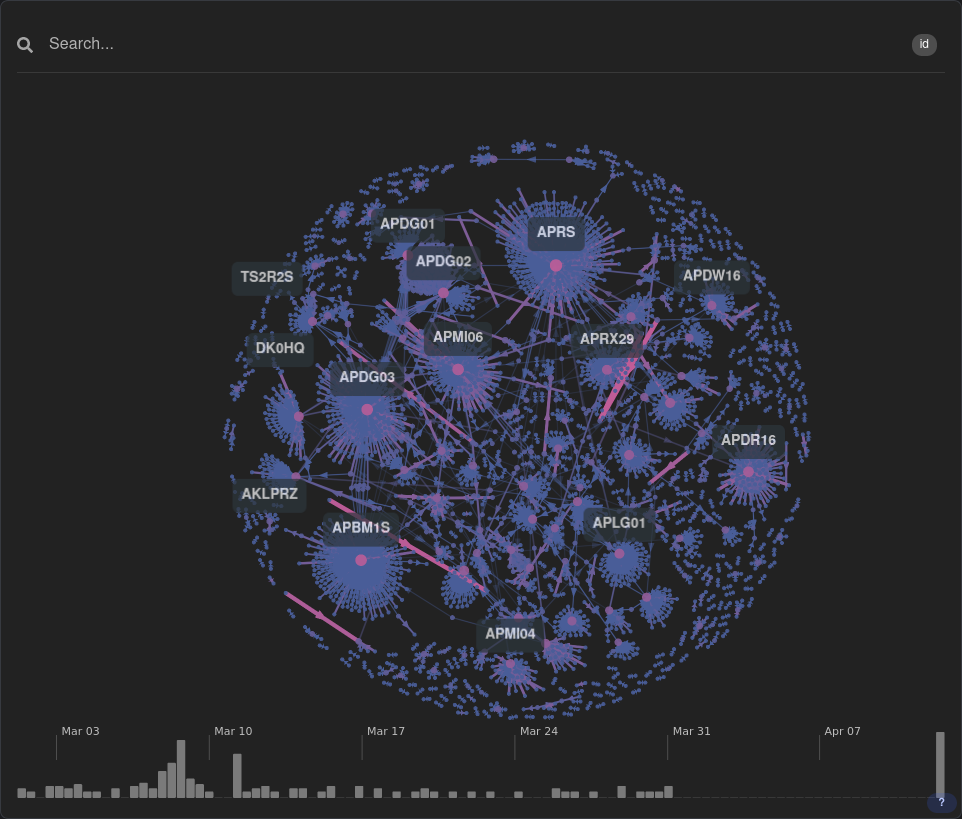
\includegraphics[width=0.85\textwidth]{Imagenes/Chapter_4/graph.png}
	\caption[Grafo de estaciones APRS.]{Grafo de estaciones APRS (elaboración propia).}
	\label{fig:graph}
\end{figure}

Las características que se buscaban en la solución final eran:

\begin{itemize}
	\item \textbf{Interactividad:} Se buscaba un grafo interactivo que permitiera al usuario explorar las relaciones entre las estaciones APRS.
	\item \textbf{Rendimiento:} Quizás la característica más importante, el grafo debía ser capaz de mostrar una gran cantidad de estaciones y conexiones sin afectar al rendimiento de la aplicación.
	\item \textbf{Personalización:} Se buscaba un grafo que permitiera personalizar la apariencia y el comportamiento de los nodos y aristas según las características de cada estación y mensaje.
\end{itemize}
Para alcanzar la solución final que se presenta ahora en la página, se han probado muchas opciones que se han ido descartando por diferentes motivos.
\subsubsection*{Alternativas probadas}
En un primer momento se intentó utilizar la librería \textbf{Networkx} de Python para la creación del grafo, sin embargo, se descartó debido a su rendimiento y a su falta de interactividad. Posteriormente se intentó utilizar la librería \textbf{Cytoscape} que es la solución por defecto que ofrece Dash, esta ofrece una gran cantidad de funcionalidades para la creación de grafos interactivos, sin embargo, se descartó de nuevo debido a su pobre rendimiento.

Una de las alternativas que también se probó fue la librería \textbf{Sigma JS} que ofrece una gran cantidad de funcionalidades y personalización para la creación de grafos interactivos. Esta librería cuenta con una funcionalidad interesante \textit{forceAtlas2} que permite calcular mediante una simulación de fuerzas la posición de los nodos y aristas en el grafo. Sin embargo, de nuevo se descartó debido a su rendimiento con una gran cantidad de nodos y aristas.

Finalmente se optó por la librería \textbf{Cosmograph JS}. Cosmograph utiliza la librería \textit{Cosmos} de cálculo de posiciones mediante la GPU y por tanto puede manejar un gran número de nodos y aristas.

\subsubsection*{El Grafo}
El problema principal con Cosmograph ha sido la falta de documentación, debido a que es una librería bastante joven, y la dificultad de integrarla con Dash. Esta librería está publicada en NPM (el repositorio de librerias de JavaScript) y se ha tenido que utilizar bundle.js para convertir el código de JavaScript en un solo fichero que se pueda importar en Dash. Ha sido necesario modificar el código fuente de la librería para terminar de integrarla con Dash.

Se han utilizado tres componentes de Cosmograph JS para la creación del grafo, el componente \textit{Cosmograph} que crea el grafo, el componente \textit{CosmographSearch} que permite mediante una barra de búsqueda encontrar una estación y el componente \textit{CosmographTimeline} que permite filtrar el grafo por rango de fechas.

Para mejorar el rendimiento general de la web se ha utilizado la técnica de \textit{lazy-loading}, que consiste en cargar los componentes del grafo solo cuando el usuario presiona el botón \textit{Load graph}. En el momento que el usuario presiona el botón, se activa un \textit{callback} de cliente de Dash. El \textit{callback} primero lee los datos del grafo de un fichero CSV que se actualiza diariamente mediante Apache Airflow. Posteriormente se crean los nodos y las aristas y se inicializa el grafo, la barra de búsqueda y la barra de tiempo. Seguidamente se establecen los parámetros de la simulación de fuerzas y se inicia la simulación. Por último se establecen las propiedades visuales y funcionales de los nodos y aristas.

Cuando el usuario posiciona el cursor sobre un nodo, se muestra un recuadro con el nombre de la estación. Cuando el usuario hace clic en un nodo, se le redirige a la página \textbf{station} de la estación seleccionada.

\section{Orquestación}

En esta sección se describe con detalle la metodología de orquestación de tareas y flujos de trabajo de la aplicación que se han ido comentando a lo largo del capítulo.

\subsection{Supervisord}
Supervisord es un sistema de control de procesos para sistemas operativos tipo Unix, diseñado para iniciar, detener y gestionar procesos de manera sencilla y robusta.

Se ha utilizado Supervisord como gestor de procesos para ejecutar en modo demonio como se ha mencionado previamente el sistema de recepción de paquetes APRS. Se ha establecido en la configuración de Supervisord que el sistema de recepción de paquetes se ejecute en el arranque del sistema y siempre después de que la interfaz de red esté disponible. En caso de fallo del sistema de recepción, Supervisord reiniciará el sistema y registrará la causa del fallo.

\subsection{Apache Airflow}
Apache Airflow es una plataforma de orquestación de tareas y flujos de trabajo. Es similar a Cron de Unix, pero permite al usuario una mayor personalización y un mayor control sobre las tareas que controla. La unidad de ejecución en Apache Airflow es el DAG (\textit{Directed Acyclic Graph}). Las tareas se definen en archivos individuales y al igual que en otros sistemas se pueden definir dependencias entre tareas.

Apache Airflow se ha utilizado para orquestar todas las tareas que permiten que APRSINT funcione correctamente se presenta en la Tabla \ref{tab:airflow-sched} la lista de los DAG que se ejecutan diariamente.

\begin{table}[htbp]
	\centering
	\begin{tabular}{|c|c|m{5.5cm}|}
		\hline
		\textbf{Hora de ejecución} & \textbf{DAG}     & \textbf{Descripción}                           \\
		\hline
		3:00 am                    & upload\_files    & Sube todos los archivos al S3 aprsinput        \\
		\hline
		5:00 am                    & download\_files  & Descarga todos los archivos a la carpeta local \\
		\hline
		7:00 am                    & insert\_database & Inserta todos los mensajes en la BBDD          \\
		\hline
		9:00 am                    & cache\_data      & Precalcula en archivos los datos para la web   \\
		\hline
	\end{tabular}
	\caption{Esquema de orquestación con Apache Airflow.}
	\label{tab:airflow-sched}
\end{table}

Por defecto Apache Airflow utiliza una base de datos SQLite para almacenar los metadatos de las tareas y los flujos de trabajo. Sin embargo, para este proyecto se ha optado por utilizar una base de datos PostgreSQL para almacenar los metadatos de Apache Airflow. Esto se ha hecho para mejorar la escalabilidad y sobre todo la fiabilidad del sistema.

Se ha creado también un usuario en la base de datos de PostgreSQL con permisos de lectura y escritura para Apache Airflow. Se ha configurado Apache Airflow para que utilice esta base de datos y este usuario en el archivo de configuración de Apache Airflow.

Otra configuración importante que se ha realizado en Apache Airflow es el cambio del ejecutor por defecto de SequentialExecutor a LocalExecutor. El ejecutor por defecto de Apache Airflow es SequentialExecutor, que ejecuta las tareas de manera secuencial en un solo hilo. Sin embargo, no se recomienda el uso de este ejecutor\footnote{\url{https://airflow.apache.org/docs/apache-airflow/stable/core-concepts/executor/sequential.html}} por lo que para mejorar el rendimiento y la escalabilidad del sistema se ha optado por utilizar LocalExecutor, que ejecuta las tareas de manera paralela en varios hilos.

Se presenta en la \Cref{fig:airflow-dashboard} la interfaz de Apache Airflow con los DAG's que se ejecutan diariamente.

\begin{figure}[h]
	\centering
	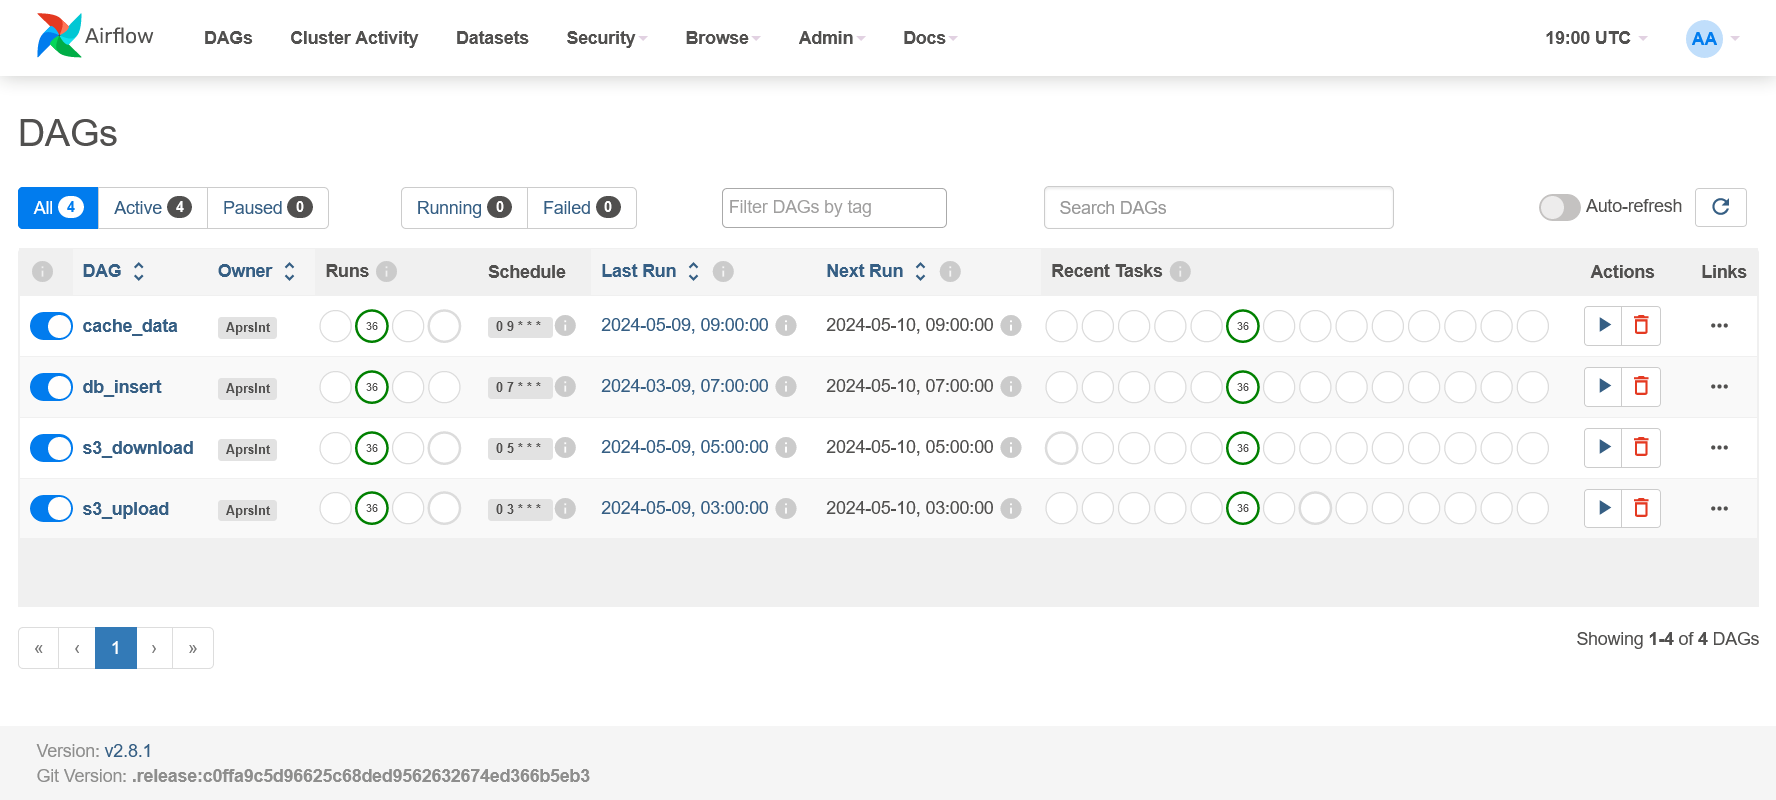
\includegraphics[width=1\textwidth]{Imagenes/Chapter_4/airflow_dashboard.png}
	\caption[Interfaz de Apache Airflow.]{Interfaz de Apache Airflow (elaboración propia).}
	\label{fig:airflow-dashboard}
\end{figure}

\section{Alojamiento}
Para alojar tanto la aplicación web como el sistema de recepción de paquetes y la base de datos de APRSINT se ha optado por utilizar una Raspberry Pi 4 conectada a un internet residencial.

Para evitar los problemas que suponen las direcciones dinámicas se ha decidido por utilizar el servicio de DNS dinámico de no-ip que permite asignar un nombre de dominio a una dirección ip dinámica. Este sistema se ha configurado en el router de modo que cuando la dirección ip cambia, el router notifica a no-ip y este actualiza el registro DNS asociado a la ip antigua por la nueva dirección.

Se ha configurado también la redirección de puertos en el router para permitir el acceso a la Raspberry Pi desde el exterior. Los servidores que se encuentran actualmente en la Raspberry Pi son:
\begin{itemize}
	\item \textbf{Servidor Web:} Se ha configurado un servidor web Nginx para servir la aplicación web de APRSINT.
	\item \textbf{Base de Datos:} Se ha configurado un servidor PostgreSQL para almacenar los metadatos de Apache Airflow y los datos de los mensajes APRS.
	\item \textbf{Apache Airflow:} Se ha configurado un servidor Apache Airflow para orquestar las tareas y flujos de trabajo de APRSINT.
	\item \textbf{Servidor SSH:} Se ha configurado un servidor SSH para permitir el acceso remoto a la Raspberry Pi y realizar todo el desarrollo.
\end{itemize}

\subsection{Servidor Web}

En esta sección se describen las tecnologías y la arquitectura del servidor web que aloja la aplicación web de APRSINT \cite{WebServer}. La aplicación utiliza el \textit{framework} Flask como \textit{backend} web, junto con Gunicorn como servidor web WSGI y Nginx como reverse proxy.

\subsubsection*{Flask}

Flask es un \textit{framework} web ligero para Python que proporciona herramientas para crear aplicaciones web de forma rápida y sencilla. En esta aplicación, Flask se utiliza como el \textit{framework} \textit{backend} para la aplicación de Dash. Proporciona las rutas y la lógica de negocio necesarias para la aplicación.

\subsubsection*{Gunicorn}

Gunicorn es un servidor HTTP WSGI (\textit{Web Server Gateway Interface}) para Python. Se utiliza para servir la aplicación Flask de forma eficiente y escalable. Gunicorn gestiona múltiples procesos de forma paralela, lo que mejora el rendimiento de la aplicación.

Para APRSINT se ha configurado Gunicorn para ejecutar la aplicación Flask en modo demonio y con 4 procesos de trabajo. Gunicorn crea un \textit{socket} UNIX en el que escucha las solicitudes HTTP y las reenvía a la aplicación Flask para su procesamiento.

\subsubsection*{Nginx}

Nginx es un servidor web de código abierto que en este caso se ha utilizado como proxy inverso. Actúa como intermediario entre los clientes y el servidor Flask / Gunicorn. Nginx se encarga de recibir las solicitudes HTTP, dirigirlas al servidor Gunicorn y devolver las respuestas a los clientes. Nginx maneja tareas como el balanceo de carga, el almacenamiento en caché la compresión de archivos y la seguridad. Se ha configurado Nginx para servir la aplicación web de APRSINT en el puerto 80 (local).

El diagrama de la arquitectura del servidor web se muestra en la \Cref{fig:web-server}. Como se puede observar, la solicitud HTTP del cliente pasa a través de Nginx, que actúa como un proxy inverso y la reenvía a Gunicorn, donde se ejecuta la aplicación Flask. Una vez que Flask procesa la solicitud, la respuesta se envía de vuelta al cliente a través de Nginx.

\begin{figure}[h]
	\centering
	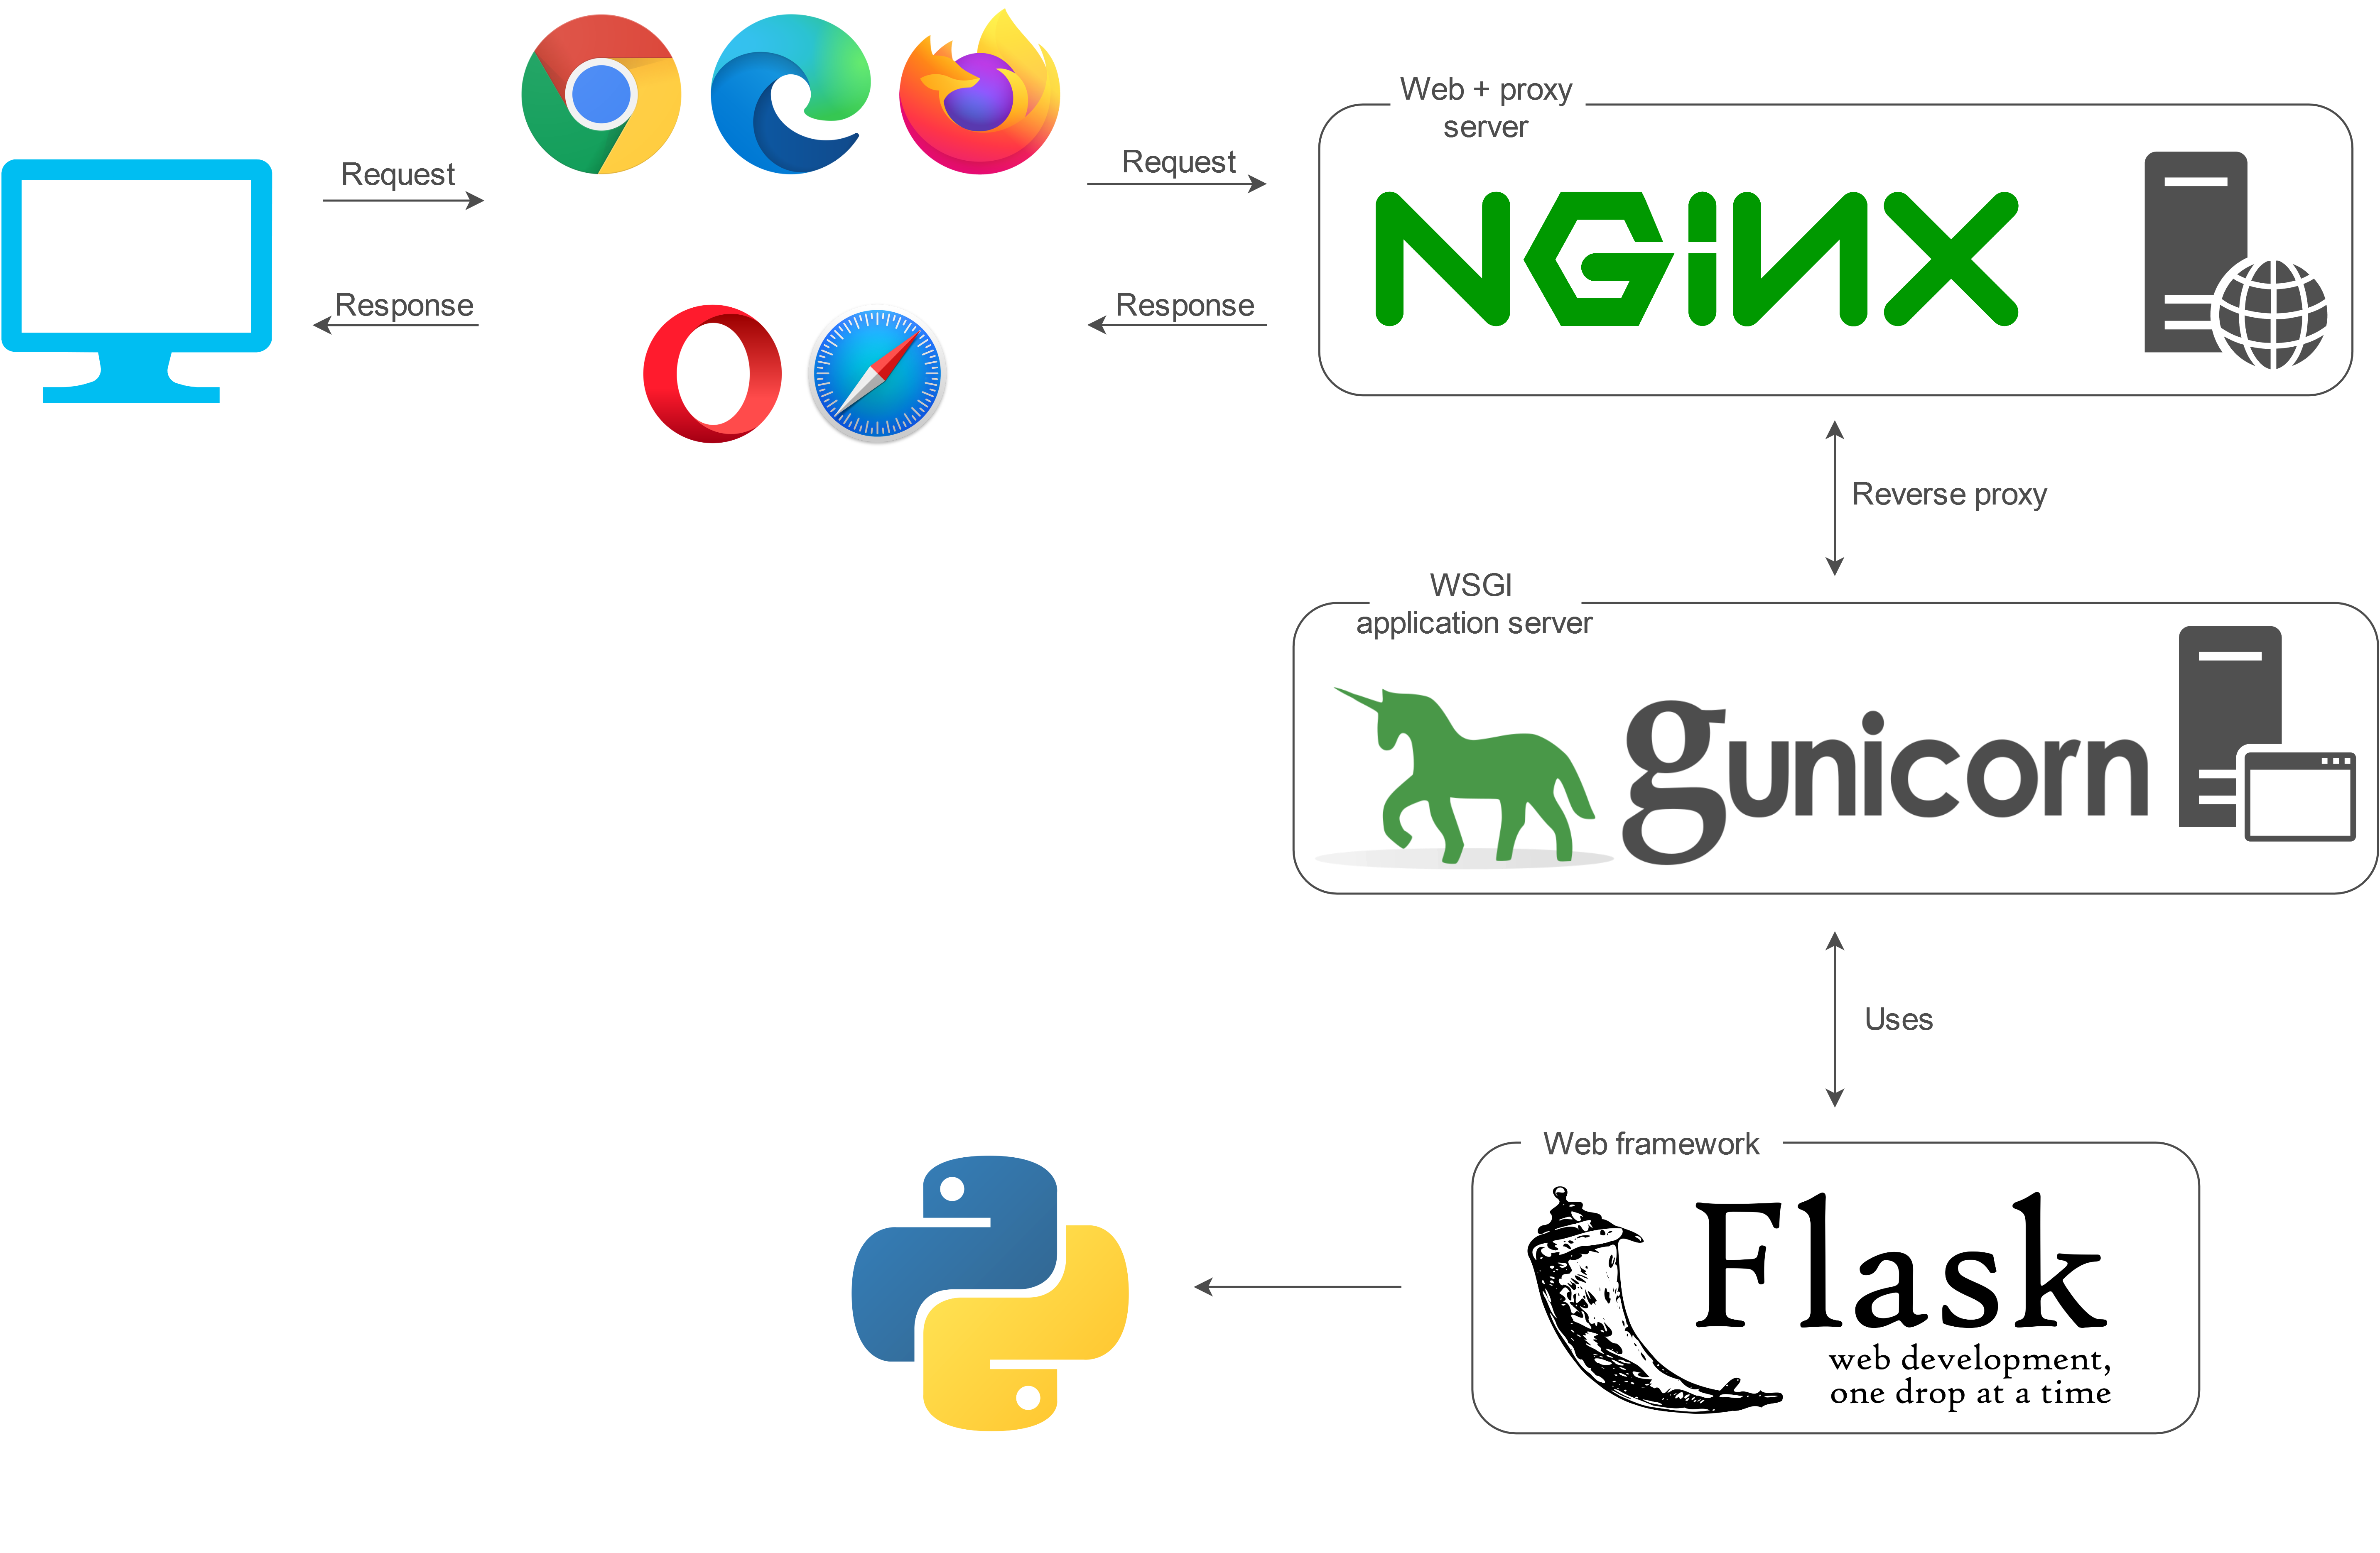
\includegraphics[width=0.9\textwidth]{Imagenes/Chapter_4/web_server.png}
	\caption[Arquitectura del servidor web de APRSINT.]{Arquitectura del servidor web de APRSINT (elaboración propia).}
	\label{fig:web-server}
\end{figure}

\subsubsection*{Flujo de una petición HTTP}

A continuación se describe cómo se maneja una solicitud HTTP desde se recibe en Nginx hasta que se envía la respuesta de vuelta al cliente. A continuación se detalla el proceso paso a paso:

\begin{enumerate}
	\item Un usuario busca en su navegador la aplicación web de APRSINT.
	\item La solicitud llega al servidor Nginx, que actúa como el servidor frontal.
	\item Nginx examina la solicitud y determina que está destinada a la aplicación Dash, por lo que la reenvía al servidor Gunicorn.
	\item Gunicorn recibe la solicitud y la asigna a uno de sus 4 procesos de Flask para su procesamiento.
	\item La aplicación Flask ejecuta la lógica correspondiente a la solicitud, que incluyen el acceso a la base de datos, y la generación del contenido de la página.
	\item Una vez que la lógica de la aplicación Flask se ha completado, se genera una respuesta.
	\item La respuesta se envía de vuelta a Gunicorn, que la reenvía a Nginx.
	\item Nginx recibe la respuesta y la devuelve al cliente que realizó la solicitud original.
\end{enumerate}

Este proceso asegura que las solicitudes sean manejadas de manera eficiente y escalable, garantizando una experiencia de navegación más fluida.

\subsection{Protección ante ataques}

En el desarrollo de la aplicación, se ha priorizado la seguridad como un aspecto fundamental. Se han implementado varias medidas \cite{RpiSecure} para proteger el sistema contra posibles ataques externos e internos. A continuación, se detallan algunas de las estrategias de seguridad utilizadas:

\begin{itemize}
	\item \textbf{Uso del protocolo SSH:} Se ha optado por utilizar exclusivamente el protocolo SSH (\textit{Secure Shell}) para la administración y desarrollo remoto de la Raspberry Pi. El SSH proporciona una conexión segura y cifrada, lo que reduce el riesgo de interceptación de datos sensibles durante la comunicación.

	\item \textbf{Creación de un usuario no root:} Se ha creado un usuario no \textit{root} con privilegios limitados para las operaciones diarias. Esto ayuda a mitigar el impacto de posibles vulnerabilidades en el sistema, ya que el acceso de usuario se limita a las funciones esenciales.

	\item \textbf{Cambio del puerto SSH por defecto:} Como medida adicional de seguridad, se ha cambiado el puerto predeterminado del servicio SSH. Esto dificulta los intentos de acceso no autorizado, ya que los atacantes suelen escanear los puertos estándar en busca de vulnerabilidades.

	\item \textbf{Desactivación del acceso por contraseña:} Se ha desactivado el acceso por contraseña al servidor SSH, lo que significa que los usuarios deben autenticarse mediante claves SSH. Este enfoque reduce el riesgo de ataques de fuerza bruta dirigidos a contraseñas débiles.

	\item \textbf{Instalación de fail2ban:} Se ha instalado y configurado fail2ban, una herramienta de prevención de intrusiones que monitoriza los registros del sistema en busca de intentos de acceso fallidos. Fail2ban bloquea automáticamente las direcciones ip de los atacantes después de un número especificado de intentos fallidos, lo que ayuda a proteger contra ataques de fuerza bruta.

	\item \textbf{Configuración de un firewall UFW:} Se ha configurado el firewall UFW (\textit{Uncomplicated Firewall}) para controlar el tráfico de red entrante y saliente. El firewall UFW bloquea el acceso a los puertos no utilizados y permite especificar reglas de acceso para servicios específicos, lo que ayuda a prevenir intrusiones no autorizadas.

	\item \textbf{Actualizaciones regulares del sistema:} Se ha establecido un \textit{cronjob} para que actualice el sistema operativo y las aplicaciones instaladas regularmente. Las actualizaciones de seguridad y los parches de \textit{software} son esenciales para proteger el sistema contra vulnerabilidades conocidas.
\end{itemize}

\noindent Mediante estas estrategias, se pretende minimizar los riesgos de seguridad y proteger la integridad y la confidencialidad de los datos de la aplicación.

\section{Casos de uso}

En esta sección se describen los casos de uso de la aplicación web de APRSINT, incluyendo los actores, las funcionalidades y los escenarios de uso. Para esto, se han identificado a dos posibles actores que utilizarían la aplicación web de APRSINT:
\begin{itemize}
	\item \textbf{Investigador de OSINT:} Este actor utiliza funciones avanzadas de filtrado para analizar y extraer inteligencia de los datos APRS. El investigador busca obtener información detallada a partir de los mensajes transmitidos, utilizando herramientas para explorar patrones, tendencias y relaciones en los datos.
	\item \textbf{Radioaficionados curiosos:} Son entusiastas de la radioafición que visitan APRSINT principalmente por curiosidad y para explorar el mundo de APRS de una manera más interactiva y visual. Aunque pueden no tener experiencia en análisis avanzado de datos, están interesados en descubrir nuevas estaciones, rutas de seguimiento y eventos en tiempo real utilizando la plataforma.
\end{itemize}

\noindent Se han identificado las siguientes funcionalidades y escenarios de uso para la aplicación web de APRSINT:
\begin{itemize}
	\item \textbf{Visualización de estaciones APRS:} Los usuarios de la aplicación pueden visualizar las estaciones APRS en un mapa interactivo, proporcionando una representación geográfica del panorama APRS.
	\item \textbf{Filtrado de estaciones APRS:} Permite a los usuarios filtrar las estaciones APRS según criterios específicos, como rango de fechas, país, contenido del mensaje, tipo de estación y SSID, para obtener información relevante.

	\item \textbf{Búsqueda de mensajes:} Se pueden buscar mensajes emitidos por las estaciones que contengan una palabra o frase específica, facilitando la localización de información relevante en la red APRS.

	\item \textbf{Visualización de información detallada de una estación APRS:} Esta funcionalidad permite acceder a información detallada de una estación APRS en particular, incluyendo datos de identificación, posiciones reportadas y mensajes emitidos, para un análisis más profundo.

	\item \textbf{Visualización del grafo de estaciones APRS:} Los usuarios pueden visualizar un grafo que representa las conexiones entre las estaciones APRS, proporcionando una visualización clara de la estructura de la red APRS.

	\item \textbf{Exploración del grafo de estaciones APRS:} Permite la exploración del grafo de estaciones APRS interactuando con los nodos y enlaces, obteniendo información adicional sobre las relaciones entre las estaciones.

	\item \textbf{Descarga de datos:} Facilita la descarga de los datos de las estaciones APRS en formato CSV, facilitando su análisis fuera de la plataforma APRSINT.

\end{itemize}

\noindent Estas son las funcionalidades y escenarios de uso que se han diseñado para satisfacer las necesidades de los dos actores y proporcionar una experiencia completa en APRSINT.
%\include{Capitulos/Capitulo4}
%\include{Capitulos/Capitulo5}
\chapter{Conclusiones y trabajo futuro}
\label{cap:conclusiones}

\section{Conclusiones}

En este trabajo se ha presentado un sistema completo centrado en la adquisición, procesamiento, análisis y visualización de datos APRS. A lo largo del proyecto, se ha seguido una metodología de trabajo dinámica y flexible que ha permitido adaptarse a los problemas encontrados durante el desarrollo.

Considero que los objetivos planteados al inicio del proyecto se han cumplido con éxito. La solución propuesta se ha desarrollado siguiendo un enfoque modular y escalable, lo que permite una fácil extensión y adaptación a futuras necesidades. Además, se ha priorizado la usabilidad y la experiencia del usuario.

\subsection{Éxitos del proyecto}

Durante el desarrollo de este proyecto, se han alcanzado varios éxitos significativos. En primer lugar, se ha logrado implementar un sistema completo que cumple con los requisitos establecidos al inicio del proyecto. Esto incluye la adquisición eficiente de datos APRS, un procesamiento y análisis detallado y una visualización clara de la información. Además, el volumen de datos que maneja APRSINT está a la par con otras soluciones comerciales, lo que demuestra la robustez de la implementación a pesar de ser Open-Source.

Además, el enfoque modular y escalable adoptado en el desarrollo de la solución ha demostrado ser efectivo, ya que a lo largo del desarrollo ha facilitado la incorporación de nuevas funcionalidades y la adaptación sencilla a los cambios que han ido ocurriendo a lo largo del proyecto. 

\subsection{Desafíos superados}

A pesar de los éxitos alcanzados, también se han enfrentado varios desafíos y obstáculos durante el desarrollo de este proyecto.

Uno de los principales desafíos encontrados fue el intento inicial de utilizar dispositivos RTL-SDR para la adquisición de datos APRS, lo que resultó en problemas técnicos y de estabilidad\footnote{En las fechas en las que comenzó el proyecto, el \textit{Digipeater} de la zona estaba apagado y no se recibía nada de información}. Este desafío se ha superado utilizando la red APRS-IS para la adquisición de datos lo que ha resultado ser mucho más eficiente y confiable y sobre todo, mucho más versátil, ya que se pueden obtener datos de cualquier parte del mundo sin necesidad de tener un dispositivo físico en la zona de interés

Otro de los desafíos que ha habido que superar ha sido el de la limitación del \textit{hardware}. Como se ha mencionado anteriormente, la Raspberry Pi utilizada no podía soportar el procesamiento masivo de datos APRS además de la carga que tenía por los otros módulos de la aplicación. Para superar esta limitación, se implementó una solución que transfiere el procesamiento al cloud de AWS. Esto ha acelerado el procesamiento y ha aligerado la carga de cómputo de la Raspberry Pi.

Quizá el desafío más importante del proyecto ha sido la gestión de recursos y tiempo, ya que este ha sido un proyecto unipersonal ambicioso. La óptima gestión y planificación del tiempo han resultado ser fundamentales para superar este desafío y completar el proyecto con éxito.

\subsection{Aprendizajes del proyecto}

El proyecto ha sido una experiencia de aprendizaje valiosa en multitud de aspectos. En primer lugar, he adquirido una comprensión más profunda de los sistemas de comunicación de radioaficionados y de la tecnología APRS. Además he trabajado con tecnologías y herramientas nuevas para mí, como puede ser el cloud AWS o sistemas de orquestación como Apache Airflow, que me han permitido ampliar mis habilidades técnicas. Finalmente considero que el aprendizaje más importante ha sido el de la gestión de un proyecto de esta envergadura, desde la planificación inicial hasta la implementación y la entrega final.

\subsection{Limitaciones del proyecto}

A pesar de los éxitos y logros alcanzados, también hay algunas limitaciones en la solución propuesta. Una de las limitaciones más importantes es la dependencia de la red APRS-IS para la adquisición de datos, lo que puede limitar la cobertura y la precisión de los datos recopilados. Además, la solución actual no es capaz de manejar grandes volúmenes de datos en tiempo real, lo que puede limitar su utilidad en entornos de alta demanda. 

\section{Trabajo futuro}

En resumen, considero que el proyecto ha sido satisfactorio y que la solución propuesta tiene un gran potencial para mejorar la experiencia de los usuarios de APRS y enriquecer la información disponible. Para el trabajo futuro, se pueden considerar varias áreas de mejora y expansión.

Una posible área de desarrollo futuro es la integración de tecnologías, como el aprendizaje automático e inteligencia artificial, para mejorar la precisión y las capacidades de análisis del sistema, facilitando la detección de patrones y otros elementos interesantes. Además, se puede explorar la posibilidad de ampliar la funcionalidad de la solución para incluir características adicionales solicitadas por los usuarios o identificadas durante el uso continuo del sistema.

Además, el sistema puede ser extendido fácilmente para trabajar con otros protocolos de radio, como CATS\footnote{CATS es un proyecto con el objetivo de mejorar el sistema APRS} o LoRa, lo que ampliaría su alcance y utilidad en diferentes entornos de comunicación. También se puede mejorar la capacidad de filtrado del sistema, permitiendo a los usuarios definir y aplicar una variedad más amplia de filtros para adaptarse a sus necesidades específicas de análisis de datos.

Otra área de mejora importante es la expansión de las fuentes de datos APRS utilizadas por el sistema. Actualmente, el sistema utiliza los datos provenientes de la red APRS-IS, lo que podría no capturar todos los paquetes APRS transmitidos si no llegan a un I-Gate. Para abordar esto, se pueden explorar otras fuentes de datos, como la integración con dispositivos RTL-SDR, la integración directa con estaciones de radio APRS locales o la colaboración con otros sistemas APRS existentes para mejorar la cobertura y la precisión de los datos recopilados.

Finalmente, se puede considerar escalar el sistema para utilizar \textit{hardware} más capaz, lo que mejoraría su rendimiento y capacidad de procesamiento. Esto implicaría el uso de servidores más potentes o la distribución de la carga de procesamiento en múltiples nodos, lo que permitiría manejar volúmenes de datos más grandes y complejos de manera más eficiente.





%%%%%%%%%%%%%%%%%%%%%%%%%%%%%%%%%%%%%%%%%%%%%%%%%%%%%%%%%%%%%%%%%%%%%%%%%%%
% Si el TFG se escribe en inglés, comentar las siguientes líneas 
% porque no es necesario incluir nuevamente las Conclusiones en inglés
\begin{otherlanguage}{english}
\chapter*{Introduction}
\label{cap:introduction}
\addcontentsline{toc}{chapter}{Introduction}

\chapterquote{People think of education as something that they can finish.}{Isaac Asimov}
\section{What is APRS?}

APRS or \textit{Automatic Packet Reporting System} is a real-time digital communications system that allows the exchange of information between amateur radio stations.

In general, APRS is used for vehicle tracking, transmission of text messages, broadcasting of weather information and to aid communication in emergency situations, although due to the flexibility of the protocol it can be used in any other situation.

\begin{figure}[h!]
	\centering
	
\includegraphics[width=0.25\textwidth]{Imagenes/Chapter_1/APRS_logo.png}
	\caption{APRS logo.}
	\label{fig:aprs-logo-en}
\end{figure}

\section{Main APRS features}

APRS has several features that make it useful and versatile in the field of amateur radio communication, among which are the following:
\begin{itemize}
	\item \textbf{Working frequency:} APRS operates in the VHF band, specifically on the 144.80 MHz frequency in Europe, although other regions of the world use different frequencies as shown in the figure below. \Cref{fig:freq-map-en}.
	\item \textbf{Transmission mode:} APRS uses as a transmission mode individual packets that have to follow an established format, which greatly facilitates the adoption and integration of this technology.
	\item \textbf{APRS retransmission policy:} In the APRS system, a packet of information is transmitted multiple times, gradually decreasing the emission frequency of these transmissions as time progresses. This method aims to maximize the packet reception rate.
\end{itemize}

\begin{figure}[h]
	\centering
	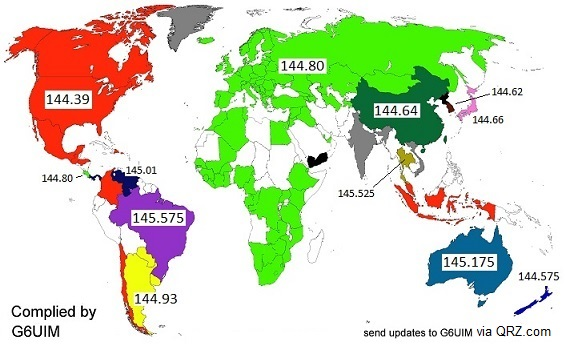
\includegraphics[width=0.6\textwidth]{Imagenes/Chapter_1/mapa_frecuencias_aprs.jpg}
	\caption{APRS emission frequency around the globe.}
	\label{fig:freq-map-en}
\end{figure}


\section{Main APRS applications}

\begin{itemize}
	\item \textbf{GPS position reports:} APRS allows users to send their geographic location in the form of coordinates, obtained through GPS systems, which facilitates the tracking of vehicles or people in real time.

	\item \textbf{Weather data:} Weather stations often use APRS messages to report different data such as temperature, humidity or barometric pressure, including updated and useful information for various applications.

	\item \textbf{Internet integration:} Through the APRS-IS system, APRS messages are accessible over the Internet through different nodes, extending the reach and scope of this system.

	\item \textbf{Uso en Emergencias:} In emergency situations, APRS is a vital tool for broadcast communication and tracking of resources and personnel.
\end{itemize}

\section{History and development of APRS}

The APRS system was born in the 1980s by Bob Bruninga, an engineer working at the U.S. Naval Academy. Bruninga created the first implementation of APRS on an Apple II computer in 1982 for the purpose of mapping Navy position reports on the high seas.\cite{APRSOrigins}

The first real use of APRS was in 1984, when Bruninga developed a more advanced version on a VIC-20 to report the position and status of horses in an endurance race.

Over the next few years, Bruninga continued to refine the system, which he later dubbed the CETS (\textit{Connectionless Emergency Traffic System}).

After a series of \textit{Federal Emergency Management Agency} (FEMA) exercises using CETS, the system was moved to the IBM PC. During the 1990s, CETS (now known as the \textit{Automatic Position Reporting System}) continued to evolve.

As GPS technology became more widely available, the term ``Positioning'' was replaced by ``Package'' to better represent the broader capabilities of the system and emphasize its uses beyond mere position reporting.

\begin{figure}[h]
	\centering
	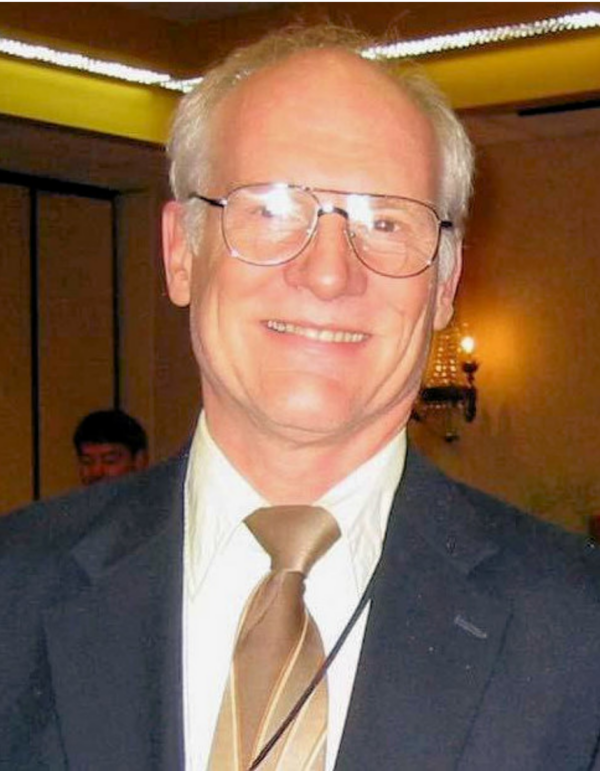
\includegraphics[width=0.2\textwidth]{Imagenes/Chapter_1/bob_bruninga.png}
	\caption{Bob Bruninga (creator of the APRS system).}
	\label{fig:bob-bruninga-en}
\end{figure}


\section{Proposal and Objectives}

A comprehensive solution is proposed to encompass the acquisition, processing, visualization, and analysis of APRS data.

\subsection{Objectives}

The aim of the project is to develop a solution that enhances user experience and enriches available APRS information through the integration of data from various open and accessible sources.

\begin{itemize}
	\item \textbf{Enhanced User Experience:} The solution will have an intuitive, fast, and useful interface that facilitates navigation and interaction with the data.
	
	\item \textbf{Advanced Analysis:} The solution will have advanced tools for detailed visualization of APRS traffic, precise filtering, and data analysis, aiming to extract intelligence from received messages.
	
	\item \textbf{Supplementation:} The solution is not aimed at replacing aprs.fi, aprs.to, or other similar platforms but to offer an alternative with complementary functionalities to add valuable insights to the user.
	
	\item \textbf{Information Enrichment:} Data from various open and available sources will be collected to offer a more comprehensive view of APRS traffic and its users, thus improving the quality of information available to users.
\end{itemize}

\subsection{Benefits}

\begin{itemize}
	\item \textbf{Better Understanding of APRS Traffic:} Users will be able to obtain more detailed and actionable information from transmitted messages, allowing them to better understand APRS traffic.
	
	\item \textbf{More Effective Decision Making:} Integrated data analysis will help users make more informed decisions based on the information received, thereby improving the effectiveness of their actions.
	
	\item \textbf{Flexibility:} The self-hosting option will allow users to have greater control over their data and privacy, providing additional flexibility in its management.
	
\end{itemize}

\section{Requirements}

The proposed solution must meet a series of essential requirements to ensure its value and accessibility:

\begin{itemize}
	\item \textbf{Low Cost:} The solution must be economical to ensure accessibility to a wide range of users, including those with limited budgets.

	\item \textbf{Hosting Flexibility:} The solution must offer self-hosting capability; users should be able to choose to host it on their own servers or use the solution in the cloud according to their preferences and specific requirements.

	\item \textbf{Extensibility:} The solution must be extensible, meaning it should allow the integration of new functionalities and expansion of its capacity according to the changing needs of users.
	
	\item \textbf{Improved Filtering:} More precise and flexible filtering should be provided compared to existing platforms, enabling users to obtain relevant and useful information from APRS data to complement that already provided by alternatives.
	
	\item \textbf{Integrated Data Analysis:} The solution must include integrated data analysis to help users better understand the information received via APRS and derive valuable insights and conclusions from transmitted messages.
	
\end{itemize}

\section{Work plan}

For the execution of this project, the following work plan has been proposed, which is divided into the following phases:

\begin{itemize}
	\item \textbf{Phase 1:} Research and Requirements Analysis.
	\item \textbf{Phase 2:} Design and Planning.
	\item \textbf{Phase 3:} Implementation and Development.
	\item \textbf{Phase 4:} Report Writing.
\end{itemize}

Figure \ref{fig:gantt-diagram-en} shows a Gantt chart with the start and end dates of each of the activities carried out throughout the project.

\begin{figure}[h]
	\centering
	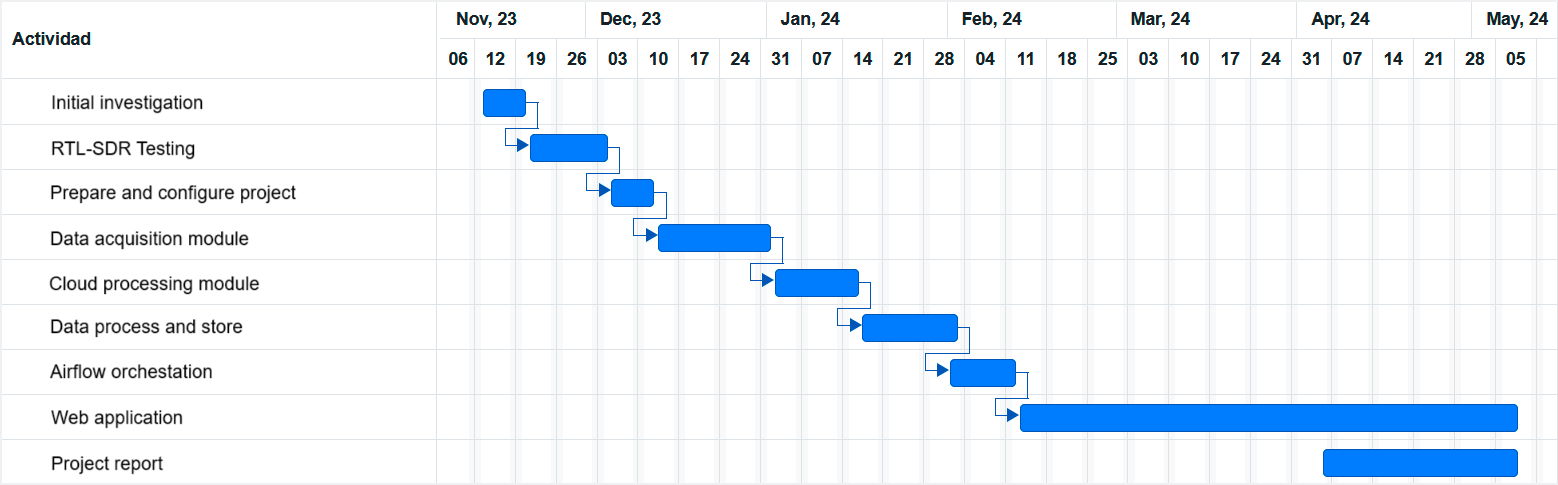
\includegraphics[width=1\textwidth]{Imagenes/Chapter_1/gant_en.png}
	\caption{Proposed work plan.}
	\label{fig:gantt-diagram-en}
\end{figure}

\noindent Regular meetings have also been held with the TFG supervisors to review progress and discuss any issues encountered during development.
\chapter*{Conclusions and future work}
\label{cap:conclusions}
\addcontentsline{toc}{chapter}{Conclusions and Future Work}

\section{Conclusions}

This work has presented a comprehensive system focused on the acquisition, processing, analysis, and visualization of APRS data. Throughout the project, a dynamic and flexible working methodology has been followed, allowing for adaptation to the challenges encountered during development.

The objectives set at the beginning of the project have been successfully achieved. The proposed solution has been developed following a modular and scalable approach, enabling easy extension and adaptation to future needs. Additionally, usability and user experience have been prioritized.

\subsection{Project successes}

Several significant successes have been achieved during the development of this project. Firstly, a complete system fulfilling the requirements established at the project's outset has been implemented. This includes efficient acquisition of APRS data, detailed processing and analysis, and clear visualization of information. Additionally, the volume of data handled by APRSINT is on par with other commercial solutions, demonstrating the robustness of the implementation despite being Open-Source.

Furthermore, the modular and scalable approach adopted in the solution's development has proven effective. Throughout development, it facilitated the incorporation of new functionalities and straightforward adaptation to changes that occurred during the project.

\subsection{Challenges overcome}

Despite the successes achieved, several challenges and obstacles were encountered during this project's development.

One of the main challenges encountered was the initial attempt to use RTL-SDR devices for APRS data acquisition, resulting in technical and stability issues\footnote{At the beginning of the project, the Digipeater in the area was offline, and no information was received}. This challenge was overcome by using the APRS-IS network for data acquisition, which proved to be much more efficient, reliable, and versatile, allowing data to be obtained from anywhere in the world without the need for a physical device in the area of interest.

Another challenge that had to be overcome was hardware limitations. As mentioned earlier, the Raspberry Pi used could not support massive APRS data processing in addition to the workload from other application modules. To overcome this limitation, a solution was implemented to offload processing to the AWS cloud. This accelerated processing and lightened the Raspberry Pi's processing load.

Perhaps the most significant challenge of the project was resource and time management, as this was an ambitious solo project. Good time management and planning proved to be crucial in overcoming this challenge and successfully completing the project.

\subsection{Project learnings}

The project has been a valuable learning experience in many aspects. Firstly, a deeper understanding of amateur radio communication systems and APRS technology has been acquired. Additionally, working with new technologies and tools, such as AWS cloud or orchestration systems like Apache Airflow, has allowed for the expansion of technical skills. Finally, the most important learning has been project management of this magnitude, from initial planning to implementation and final delivery.

\subsection{Project limitations}

Despite the successes and achievements, there are also some limitations in the proposed solution. One of the most significant limitations is the dependency on the APRS-IS network for data acquisition, which may restrict the coverage and accuracy of the collected data. Additionally, the current solution is not capable of handling large volumes of real-time data, which may limit its utility in high-demand environments.

\section{Future work}

In summary, I consider the project a success, and the proposed solution has great potential to enhance the APRS user experience and enrich available information. For future work, several areas of improvement and expansion can be considered.

One potential area for future development is the integration of technologies such as machine learning and artificial intelligence to enhance the system's accuracy and analysis capabilities, facilitating pattern detection and other interesting elements. Additionally, exploring the possibility of expanding the solution's functionality to include additional features requested by users or identified during continued system use is worthwhile.

Moreover, the system can be easily extended to work with other radio protocols, such as CATS\footnote{CATS is a project aimed at improving the APRS system} or LoRa, which would broaden its scope and utility in different communication environments. Improving the system's filtering capacity, allowing users to define and apply a wider variety of filters to suit their specific data analysis needs, is also an area for enhancement.

Another significant area for improvement is expanding the APRS data sources used by the system. Currently, the system relies mainly on data from the APRS-IS network, which may not capture all transmitted APRS packets if they do not reach an I-Gate. To address this, exploring other data sources, such as integration with rtl-sdr devices, direct integration with local APRS radio stations, or collaboration with other existing APRS systems to enhance data coverage and accuracy, is essential.

Finally, considering scaling the system to use more capable hardware would improve its performance and processing capacity. This could involve using more powerful servers or distributing processing load across multiple nodes, allowing for more efficient handling of larger and more complex data volumes.

These areas of improvement and expansion represent exciting opportunities to continue developing and enhancing the proposed solution, ensuring its relevance and usefulness in an ever-evolving technological environment.



\end{otherlanguage}
%%%%%%%%%%%%%%%%%%%%%%%%%%%%%%%%%%%%%%%%%%%%%%%%%%%%%%%%%%%%%%%%%%%%%%%%%%%

\chapter*{Contribuciones Personales}
\label{cap:contribucionesPersonales}
\addcontentsline{toc}{chapter}{Contribuciones Personales}

En caso de trabajos no unipersonales, cada participante indicará en la memoria su contribución al proyecto con una extensión de al menos dos páginas por cada uno de los participantes.

En caso de trabajo unipersonal, elimina esta página en el fichero \texttt{TFGTeXiS.tex} (comenta o borra la línea \verb|\chapter*{Contribuciones Personales}
\label{cap:contribucionesPersonales}
\addcontentsline{toc}{chapter}{Contribuciones Personales}

En caso de trabajos no unipersonales, cada participante indicará en la memoria su contribución al proyecto con una extensión de al menos dos páginas por cada uno de los participantes.

En caso de trabajo unipersonal, elimina esta página en el fichero \texttt{TFGTeXiS.tex} (comenta o borra la línea \verb|\chapter*{Contribuciones Personales}
\label{cap:contribucionesPersonales}
\addcontentsline{toc}{chapter}{Contribuciones Personales}

En caso de trabajos no unipersonales, cada participante indicará en la memoria su contribución al proyecto con una extensión de al menos dos páginas por cada uno de los participantes.

En caso de trabajo unipersonal, elimina esta página en el fichero \texttt{TFGTeXiS.tex} (comenta o borra la línea \verb|\include{Capitulos/ContribucionesPersonales}|).

\section*{Estudiante 1}
Al menos dos páginas con las contribuciones del estudiante 1.

\section*{Estudiante 2}
Al menos dos páginas con las contribuciones del estudiante 2. En caso de que haya más estudiantes, copia y pega una de estas secciones.

|).

\section*{Estudiante 1}
Al menos dos páginas con las contribuciones del estudiante 1.

\section*{Estudiante 2}
Al menos dos páginas con las contribuciones del estudiante 2. En caso de que haya más estudiantes, copia y pega una de estas secciones.

|).

\section*{Estudiante 1}
Al menos dos páginas con las contribuciones del estudiante 1.

\section*{Estudiante 2}
Al menos dos páginas con las contribuciones del estudiante 2. En caso de que haya más estudiantes, copia y pega una de estas secciones.



%
% Bibliografía
%
% Si el TFM se escribe en inglés, editar TeXiS/TeXiS_bib para cambiar el
% estilo de las referencias
%---------------------------------------------------------------------
%
%                      configBibliografia.tex
%
%---------------------------------------------------------------------
%
% bibliografia.tex
% Copyright 2009 Marco Antonio Gomez-Martin, Pedro Pablo Gomez-Martin
%
% This file belongs to the TeXiS manual, a LaTeX template for writting
% Thesis and other documents. The complete last TeXiS package can
% be obtained from http://gaia.fdi.ucm.es/projects/texis/
%
% Although the TeXiS template itself is distributed under the 
% conditions of the LaTeX Project Public License
% (http://www.latex-project.org/lppl.txt), the manual content
% uses the CC-BY-SA license that stays that you are free:
%
%    - to share & to copy, distribute and transmit the work
%    - to remix and to adapt the work
%
% under the following conditions:
%
%    - Attribution: you must attribute the work in the manner
%      specified by the author or licensor (but not in any way that
%      suggests that they endorse you or your use of the work).
%    - Share Alike: if you alter, transform, or build upon this
%      work, you may distribute the resulting work only under the
%      same, similar or a compatible license.
%
% The complete license is available in
% http://creativecommons.org/licenses/by-sa/3.0/legalcode
%
%---------------------------------------------------------------------
%
% Fichero  que  configura  los  parámetros  de  la  generación  de  la
% bibliografía.  Existen dos  parámetros configurables:  los ficheros
% .bib que se utilizan y la frase célebre que aparece justo antes de la
% primera referencia.
%
%---------------------------------------------------------------------


%%%%%%%%%%%%%%%%%%%%%%%%%%%%%%%%%%%%%%%%%%%%%%%%%%%%%%%%%%%%%%%%%%%%%%
% Definición de los ficheros .bib utilizados:
% \setBibFiles{<lista ficheros sin extension, separados por comas>}
% Nota:
% Es IMPORTANTE que los ficheros estén en la misma línea que
% el comando \setBibFiles. Si se desea utilizar varias líneas,
% terminarlas con una apertura de comentario.
%%%%%%%%%%%%%%%%%%%%%%%%%%%%%%%%%%%%%%%%%%%%%%%%%%%%%%%%%%%%%%%%%%%%%%
\setBibFiles{%
biblio%
}

%%%%%%%%%%%%%%%%%%%%%%%%%%%%%%%%%%%%%%%%%%%%%%%%%%%%%%%%%%%%%%%%%%%%%%
% Definición de la frase célebre para el capítulo de la
% bibliografía. Dentro normalmente se querrá hacer uso del entorno
% \begin{FraseCelebre}, que contendrá a su vez otros dos entornos,
% un \begin{Frase} y un \begin{Fuente}.
%
% Nota:
% Si no se quiere cita, se puede eliminar su definición (en la
% macro setCitaBibliografia{} ).
%%%%%%%%%%%%%%%%%%%%%%%%%%%%%%%%%%%%%%%%%%%%%%%%%%%%%%%%%%%%%%%%%%%%%%
\setCitaBibliografia{
\begin{FraseCelebre}
\begin{Frase}
  Citadme diciendo que me han citado mal.
\end{Frase}
\begin{Fuente}
  Groucho Marx
\end{Fuente}
\end{FraseCelebre}
}

%%
%% Creamos la bibliografia
%%
\makeBib

% Variable local para emacs, para  que encuentre el fichero maestro de
% compilación y funcionen mejor algunas teclas rápidas de AucTeX

%%%
%%% Local Variables:
%%% mode: latex
%%% TeX-master: "../Tesis.tex"
%%% End:



% Apéndices
\appendix
\chapter{Título del Apéndice A}
\label{Appendix:Key1}

Los apéndices son secciones al final del documento en las que se agrega texto con el objetivo de ampliar los contenidos del documento principal.
\chapter{Título del Apéndice B}
\label{Appendix:Key2}

Se pueden añadir los apéndices que se consideren oportunos.
%\include{Apendices/appendixC}
%\include{...}
%\include{...}
%\include{...}
\backmatter



%
% Índice de palabras
%

% Sólo  la   generamos  si  está   declarada  \generaindice.  Consulta
% TeXiS.sty para más información.

% En realidad, el soporte para la generación de índices de palabras
% en TeXiS no está documentada en el manual, porque no ha sido usada
% "en producción". Por tanto, el fichero que genera el índice
% *no* se incluye aquí (está comentado). Consulta la documentación
% en TeXiS_pream.tex para más información.
\ifx\generaindice\undefined
\else
%%---------------------------------------------------------------------
%
%                        TeXiS_indice.tex
%
%---------------------------------------------------------------------
%
% TeXiS_indice.tex
% Copyright 2009 Marco Antonio Gomez-Martin, Pedro Pablo Gomez-Martin
%
% This file belongs to TeXiS, a LaTeX template for writting
% Thesis and other documents. The complete last TeXiS package can
% be obtained from http://gaia.fdi.ucm.es/projects/texis/
%
% This work may be distributed and/or modified under the
% conditions of the LaTeX Project Public License, either version 1.3
% of this license or (at your option) any later version.
% The latest version of this license is in
%   http://www.latex-project.org/lppl.txt
% and version 1.3 or later is part of all distributions of LaTeX
% version 2005/12/01 or later.
%
% This work has the LPPL maintenance status `maintained'.
% 
% The Current Maintainers of this work are Marco Antonio Gomez-Martin
% and Pedro Pablo Gomez-Martin
%
%---------------------------------------------------------------------
%
% Contiene  los  comandos  para  generar  el índice  de  palabras  del
% documento.
%
%---------------------------------------------------------------------
%
% NOTA IMPORTANTE: el  soporte en TeXiS para el  índice de palabras es
% embrionario, y  de hecho  ni siquiera se  describe en el  manual. Se
% proporciona  una infraestructura  básica (sin  terminar)  para ello,
% pero  no ha  sido usada  "en producción".  De hecho,  a pesar  de la
% existencia de  este fichero, *no* se incluye  en Tesis.tex. Consulta
% la documentación en TeXiS_pream.tex para más información.
%
%---------------------------------------------------------------------


% Si se  va a generar  la tabla de  contenidos (el índice  habitual) y
% también vamos a  generar el índice de palabras  (ambas decisiones se
% toman en  función de  la definición  o no de  un par  de constantes,
% puedes consultar modo.tex para más información), entonces metemos en
% la tabla de contenidos una  entrada para marcar la página donde está
% el índice de palabras.

\ifx\generatoc\undefined
\else
   \addcontentsline{toc}{chapter}{\indexname}
\fi


% Generamos el índice
\printindex

% Variable local para emacs, para  que encuentre el fichero maestro de
% compilación y funcionen mejor algunas teclas rápidas de AucTeX

%%%
%%% Local Variables:
%%% mode: latex
%%% TeX-master: "./tesis.tex"
%%% End:

\fi

%
% Lista de acrónimos
%

% Sólo  lo  generamos  si  está declarada  \generaacronimos.  Consulta
% TeXiS.sty para más información.


\ifx\generaacronimos\undefined
\else
%---------------------------------------------------------------------
%
%                        TeXiS_acron.tex
%
%---------------------------------------------------------------------
%
% TeXiS_acron.tex
% Copyright 2009 Marco Antonio Gomez-Martin, Pedro Pablo Gomez-Martin
%
% This file belongs to TeXiS, a LaTeX template for writting
% Thesis and other documents. The complete last TeXiS package can
% be obtained from http://gaia.fdi.ucm.es/projects/texis/
%
% This work may be distributed and/or modified under the
% conditions of the LaTeX Project Public License, either version 1.3
% of this license or (at your option) any later version.
% The latest version of this license is in
%   http://www.latex-project.org/lppl.txt
% and version 1.3 or later is part of all distributions of LaTeX
% version 2005/12/01 or later.
%
% This work has the LPPL maintenance status `maintained'.
% 
% The Current Maintainers of this work are Marco Antonio Gomez-Martin
% and Pedro Pablo Gomez-Martin
%
%---------------------------------------------------------------------
%
% Contiene  los  comandos  para  generar  el listado de acrónimos
% documento.
%
%---------------------------------------------------------------------
%
% NOTA IMPORTANTE:  para que la  generación de acrónimos  funcione, al
% menos  debe  existir  un  acrónimo   en  el  documento.  Si  no,  la
% compilación  del   fichero  LaTeX  falla  con   un  error  "extraño"
% (indicando  que  quizá  falte  un \item).   Consulta  el  comentario
% referente al paquete glosstex en TeXiS_pream.tex.
%
%---------------------------------------------------------------------


% Redefinimos a español  el título de la lista  de acrónimos (Babel no
% lo hace por nosotros esta vez)

\def\listacronymname{Lista de acrónimos}

% Para el glosario:
% \def\glosarryname{Glosario}

% Si se  va a generar  la tabla de  contenidos (el índice  habitual) y
% también vamos a  generar la lista de acrónimos  (ambas decisiones se
% toman en  función de  la definición  o no de  un par  de constantes,
% puedes consultar config.tex  para más información), entonces metemos
% en la  tabla de contenidos una  entrada para marcar  la página donde
% está el índice de palabras.

\ifx\generatoc\undefined
\else
   \addcontentsline{toc}{chapter}{\listacronymname}
\fi


% Generamos la lista de acrónimos (en realidad el índice asociado a la
% lista "acr" de GlossTeX)

\printglossary(acronimos)

% Variable local para emacs, para  que encuentre el fichero maestro de
% compilación y funcionen mejor algunas teclas rápidas de AucTeX

%%%
%%% Local Variables:
%%% mode: latex
%%% TeX-master: "../Tesis.tex"
%%% End:

\fi

%
% Final
%
%---------------------------------------------------------------------
%
%                      fin.tex
%
%---------------------------------------------------------------------
%
% fin.tex
% Copyright 2009 Marco Antonio Gomez-Martin, Pedro Pablo Gomez-Martin
%
% This file belongs to the TeXiS manual, a LaTeX template for writting
% Thesis and other documents. The complete last TeXiS package can
% be obtained from http://gaia.fdi.ucm.es/projects/texis/
%
% Although the TeXiS template itself is distributed under the 
% conditions of the LaTeX Project Public License
% (http://www.latex-project.org/lppl.txt), the manual content
% uses the CC-BY-SA license that stays that you are free:
%
%    - to share & to copy, distribute and transmit the work
%    - to remix and to adapt the work
%
% under the following conditions:
%
%    - Attribution: you must attribute the work in the manner
%      specified by the author or licensor (but not in any way that
%      suggests that they endorse you or your use of the work).
%    - Share Alike: if you alter, transform, or build upon this
%      work, you may distribute the resulting work only under the
%      same, similar or a compatible license.
%
% The complete license is available in
% http://creativecommons.org/licenses/by-sa/3.0/legalcode
%
%---------------------------------------------------------------------
%
% Contiene la última página
%
%---------------------------------------------------------------------


% Ponemos el marcador en el PDF
\ifpdf
   \pdfbookmark{Fin}{fin}
\fi

\thispagestyle{empty}\mbox{}

Este texto se puede encontrar en el fichero Cascaras/fin.tex. Si deseas eliminarlo, basta con comentar la línea correspondiente al final del fichero TFGTeXiS.tex.

\vspace*{4cm}

\small

\hfill \emph{--¿Qué te parece desto, Sancho? -- Dijo Don Quijote --}

\hfill \emph{Bien podrán los encantadores quitarme la ventura,}

\hfill \emph{pero el esfuerzo y el ánimo, será imposible.}

\hfill 

\hfill \emph{Segunda parte del Ingenioso Caballero} 

\hfill \emph{Don Quijote de la Mancha}

\hfill \emph{Miguel de Cervantes}

\vfill%space*{4cm}

\hfill \emph{--Buena está -- dijo Sancho --; fírmela vuestra merced.}

\hfill \emph{--No es menester firmarla -- dijo Don Quijote--,}

\hfill \emph{sino solamente poner mi rúbrica.}

\hfill 

\hfill \emph{Primera parte del Ingenioso Caballero} 

\hfill \emph{Don Quijote de la Mancha}

\hfill \emph{Miguel de Cervantes}


\newpage
\thispagestyle{empty}\mbox{}

\newpage

% Variable local para emacs, para  que encuentre el fichero maestro de
% compilación y funcionen mejor algunas teclas rápidas de AucTeX

%%%
%%% Local Variables:
%%% mode: latex
%%% TeX-master: "../Tesis.tex"
%%% End:

%\end{otherlanguage}
\end{document}
